\documentclass[journal,twoside,web]{ieeecolor}
\usepackage{generic}
\usepackage{cite}
\usepackage{amsmath,amssymb,amsfonts}
\usepackage{algorithmic}
\usepackage{graphicx}
\usepackage[skip=0.333\baselineskip]{caption}
\usepackage{subcaption}
\usepackage{textcomp}
\usepackage{array}
\usepackage{siunitx}
\PassOptionsToPackage{hyphens}{url}\usepackage{hyperref}
\urlstyle{same}
\newcolumntype{L}[1]{>{\raggedright\let\newline\\\arraybackslash\hspace{0pt}}m{#1}}
\newcolumntype{C}[1]{>{\centering\let\newline\\\arraybackslash\hspace{0pt}}m{#1}}
\newcolumntype{R}[1]{>{\raggedleft\let\newline\\\arraybackslash\hspace{0pt}}m{#1}}

\def\BibTeX{{\rm B\kern-.05em{\sc i\kern-.025em b}\kern-.08em
    T\kern-.1667em\lower.7ex\hbox{E}\kern-.125emX}}
\markboth{\journalname, VOL. XX, NO. XX, May 2023}
{Cameron R. \MakeLowercase{\textit{et al.}}: SWING: An Investigation of Deep Brain Photobiomodulation (May 2023)}
\begin{document}
\title{SWING: An Investigation of Deep Brain Photobiomodulation}
\author{Cameron R. Author, \IEEEmembership{Member, IEEE}, Matthew T. Author, Bibhus L. Author, 
        Krishna S. Sponsor, \IEEEmembership{Member, IEEE}, John L. Mentor, \IEEEmembership{Member, IEEE}
\thanks{ }
\thanks{ }
\thanks{ }
\thanks{ }}

\maketitle

\begin{abstract}
Direct stimulation of neurons in the brain can potentially treat many diseases, such as Parkinson's  
or Alzheimer's disease. Direct stimulation, whether it be through electric or photonic stimulation,  
provided a way to activate neurons in the brain and treat diseases and conditions. However, this kind  
of invasive stimulation can have risks that lead to worsening the condition or cause infection.  
The Short-Wave Infrared Neuromodulation Gadget (SWING) aimed to build and test a non-invasive optical method  
of stimulation with funding provided by the KIND Laboratory's Brain IMPACT project. SWING is part of the  
two semester long Electrical and Computer Engineering capstone sequence at The Ohio State University. 

SWING used a cubic extrapolation to approximate the optical coefficients of biological tissue at 1550 nm. 
Monte Carlo eXtreme (MCX) was then used to predict the expected photon distribution and intensity throughout a model 
of the human head. MCX was ran multiple times with different positions and wavelengths using The Ohio State Supercomputer. 
MCX showed that deep brain stimulation is possible at all the wavelengths tested. Based on the MCX results, 1550nm wavelength 
is the most compelling choice for further testing.
\end{abstract}

\begin{IEEEkeywords}

\end{IEEEkeywords}

\section{Introduction}
\label{sec:introduction}
\IEEEPARstart{T}{here} are many physical issues in the brain, including Parkinson's disease and functional 
problems such as attention-deficit/hyperactivity disorder (ADHD) and depressive disorders. 
A solution to such problems that has been explored recently in the Neurotech community is one that involves a direct stimulation of  
neuronal connections in the brain \cite{b1,b2,b3}. Direct neuronal stimulation, whether it be through electric or photonic 
stimulation, provides a way to control mechanisms in the brain and treat diseases and conditions. These treatments result 
in an improvement of the effects caused by these diseases and conditions. However, most modern neuromodulation strategies 
are invasive in nature, and there are limited options for a non-invasive approach to neuromodulation for medical benefit. Many invasive 
techniques involve surgical implants and increase the risk of brain hemorrhage and worsening mental and emotional status for some patients,  
that often make the cons worse for life-threatening conditions \cite{b1,b4}. As a result, the Short-Wave Infrared Neuromodulation Gadget (SWING) 
looks to investigate a non-invasive method for neuromodulation using a near-infrared photonic stimulation method. 


\section{Methods}
\label{sec:methods}
SWING's software and simulation consisted of two main components: software for data preprocessing and simulation for modeling and photon distribution. 
The preprocessing stage involved approximating optical coefficients at 1550 nm.. Monte Carlo eXtreme (MCX) is used for simulating the 
behavior of the laser as it scatters and is absorbed through brain tissue, providing a model of photon dispersion in biological tissue using known or 
approximated optical coefficients.

\subsection{Software Preprocessing}
In the software preprocessing stage, the model approximated the optical coefficients of layers in the brain where it is unknown for 1550 nm sources. 
Optical coefficient data for the scalp, skull, gray matter (GM), and white matter (WM) are obtained from \cite{b5}. The wavelength ranges for each layer are as follows: 
scalp (805-2000 nm), skull (801-2000 nm), gray matter (400-1300 nm), and white matter (400-1300 nm). The data for scalp and skull cover the wavelength of interest 
(1550 nm), but the data for GM and WM do not. To address this, cubic extrapolation and interpolation methods are used to process the data and extrapolate the 
unknown layers to 1550 nm. 

The cubic interpolation method approximates the optical coefficients for the gray matter (GM) and white matter (WM) layers at 1550 nm based on the 
known data points. Let $x$ represent the wavelength and $y$ represent the absorption coefficient. The cubic interpolation function can be defined as follows:
\begin{equation}
    \label{eq:cubicEq1}
    y(x) = a(x-x_1)^3 + b(x-x_1)^2 + c(x-x_1) + d
\end{equation}
where $(x_1, y_1)$, $(x_2, y_2)$, $(x_3, y_3)$, and $(x_4, y_4)$ are the known data points for a specific layer (GM or WM).

To determine the coefficients $a$, $b$, $c$, and $d$, the model solves the following system of equations using the known data points:
\begin{equation}
    \label{eq:cubicEq2}
    y_1 = a(x_1-x_1)^3 + b(x_1-x_1)^2 + c(x_1-x_1) + d 
\end{equation}
\begin{equation}
    \label{eq:cubicEq3}
    y_2 = a(x_2-x_1)^3 + b(x_2-x_1)^2 + c(x_2-x_1) + d 
\end{equation}
\begin{equation}
    \label{eq:cubicEq4}
    y_3 = a(x_3-x_1)^3 + b(x_3-x_1)^2 + c(x_3-x_1) + d 
\end{equation}
\begin{equation}
    \label{eq:cubicEq5}
    y_4 = a(x_4-x_1)^3 + b(x_4-x_1)^2 + c(x_4-x_1) + d 
\end{equation}
Solving this system of equations provides the coefficients $a$, $b$, $c$, and $d$ specific to the cubic interpolation for the respective layer.

To apply the cubic interpolation in this study, Python programming language was used to process the known data points and calculate the coefficients. 
Once the coefficients are obtained, the cubic interpolation function is used to estimate the absorption coefficient at any desired wavelength within the range. 
This cubic interpolation provides a complex fit while preventing over-fitting in the initial steps. This allows extrapolation of the gray and white matter 
absorption coefficients to 1550 nm within the overlapping region (801-1300 nm), providing continuous lines for the unknown layers, as seen in Figure \ref{fig:Known}.

\begin{figure}[!htb]
    \center{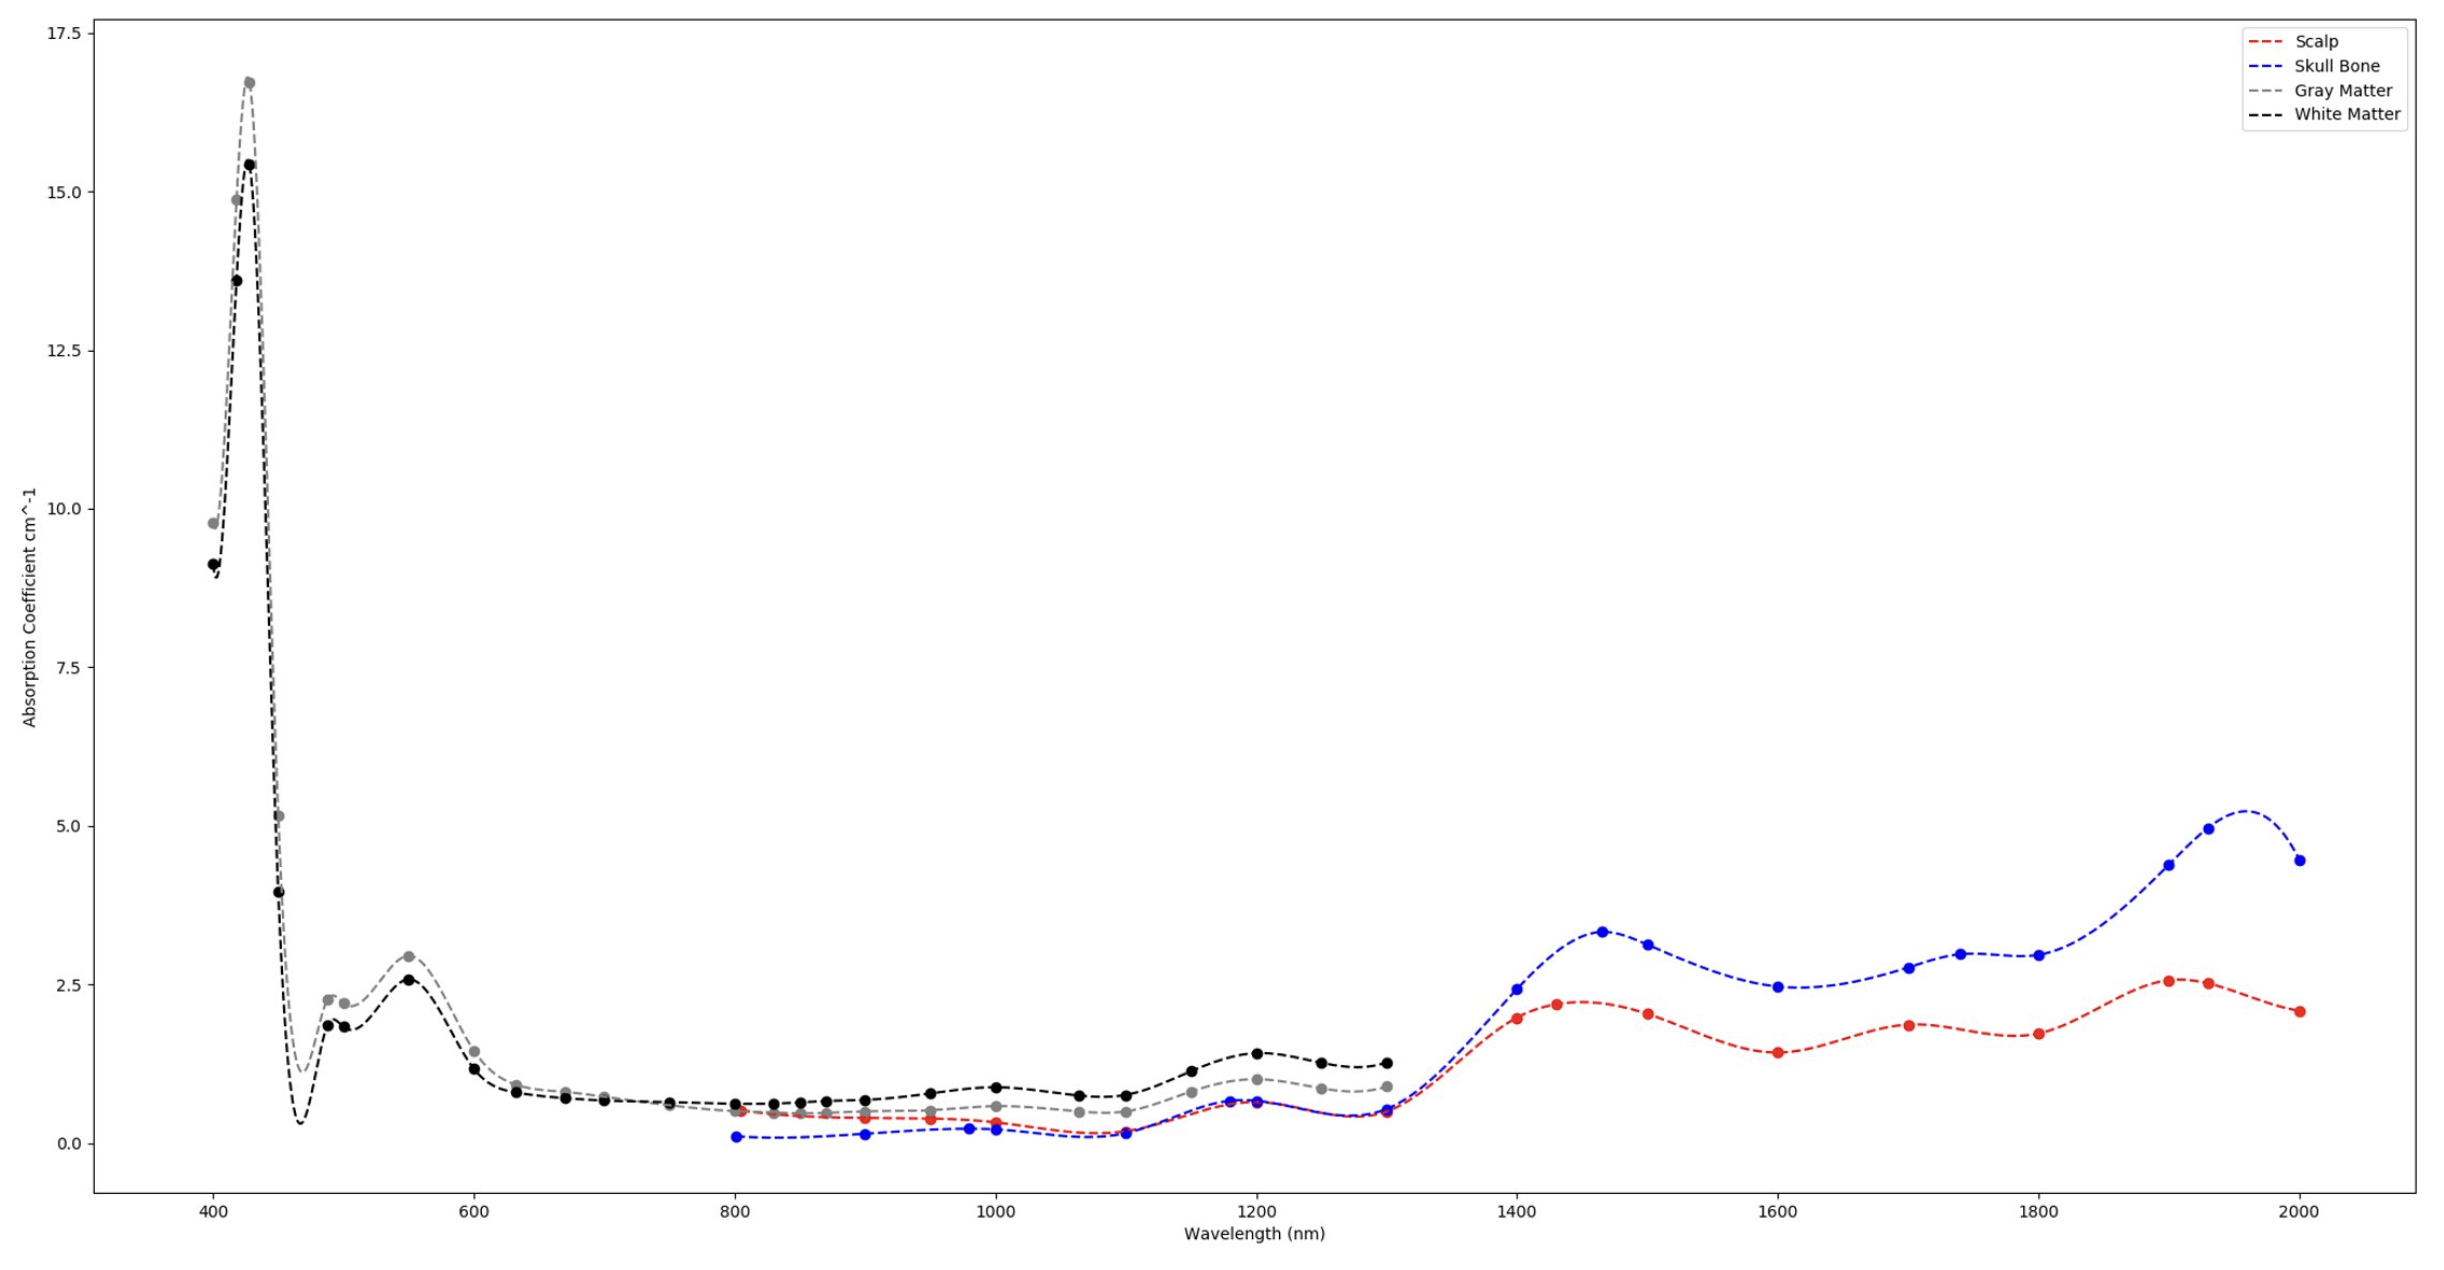
\includegraphics[width=\columnwidth]
    {Figures/KnownCoefficients.png}}
    \caption{\label{fig:Known} Cubic interpolation of known optical coefficients}
\end{figure}

To extrapolate the optical coefficients of the gray matter (GM) and white matter (WM) layers to 1550 nm, the overlapping region of the four tissues 
(801-1300 nm) is examined. Vertical offset values between the unknown layers (GM and WM) and the known layers (scalp and skull) are calculated throughout 
this overlapping region.

Let \( \lambda \) represent the wavelength and \( \mu \) represent the absorption coefficient. The vertical offset values can be calculated as the 
difference between the absorption coefficients of the unknown layers and the known layers at each wavelength in the overlapping region. 
These offset values are averaged to obtain four average vertical offsets, two for each unknown layer. Let $\overline{\mu}_{GM, Tissue}$ represent the 
average vertical offset of the gray matter based on the known $Tissue$, and $\overline{\mu}_{WM, Tissue}$ represent the average vertical offset of the white 
matter based on the known $Tissue$. The extrapolation model then extends the unknown layers by adding the previously calculated offsets to the known scalp 
and skull data.

The average vertical offsets of the gray matter and white matter can be expressed as:
\begin{equation}
    \label{eq:AvgGM}
    \begin{aligned}
    \overline{\mu}_{GM, Scalp} = \frac{1}{N} \sum_{i=1}^{N} (\mu_{\text{GM,known}}(\lambda_i) - \mu_{\text{Scalp, known}}(\lambda_i)) \\
    \overline{\mu}_{GM, Skull} = \frac{1}{N} \sum_{i=1}^{N} (\mu_{\text{GM,known}}(\lambda_i) - \mu_{\text{Skull, known}}(\lambda_i))
    \end{aligned}
\end{equation}
\begin{equation}
    \label{eq:AvgWM}
    \begin{aligned}
        \overline{\mu}_{WM, Scalp} = \frac{1}{N} \sum_{i=1}^{N} (\mu_{\text{WM,known}}(\lambda_i) - \mu_{\text{Scalp, known}}(\lambda_i)) \\
        \overline{\mu}_{WM, Skull} = \frac{1}{N} \sum_{i=1}^{N} (\mu_{\text{WM,known}}(\lambda_i) - \mu_{\text{Skull, known}}(\lambda_i))
    \end{aligned}
\end{equation}
where \( N \) represents the number of data points, \( \mu_{\text{GM,known}}(\lambda_i) \) and \( \mu_{\text{WM, known}}(\lambda_i) \) 
denote the empirical absorption coefficients at the \( i \)-th wavelength, and \( \mu_{\text{Scalp, Skull, known}}(\lambda_i) \) denotes 
the empirical absorption coefficients at the \( i \)-th wavelength within the overlapping region. This is illustrated in Figure \ref{fig:Overlap}.

\begin{figure}[!htb]
    \center{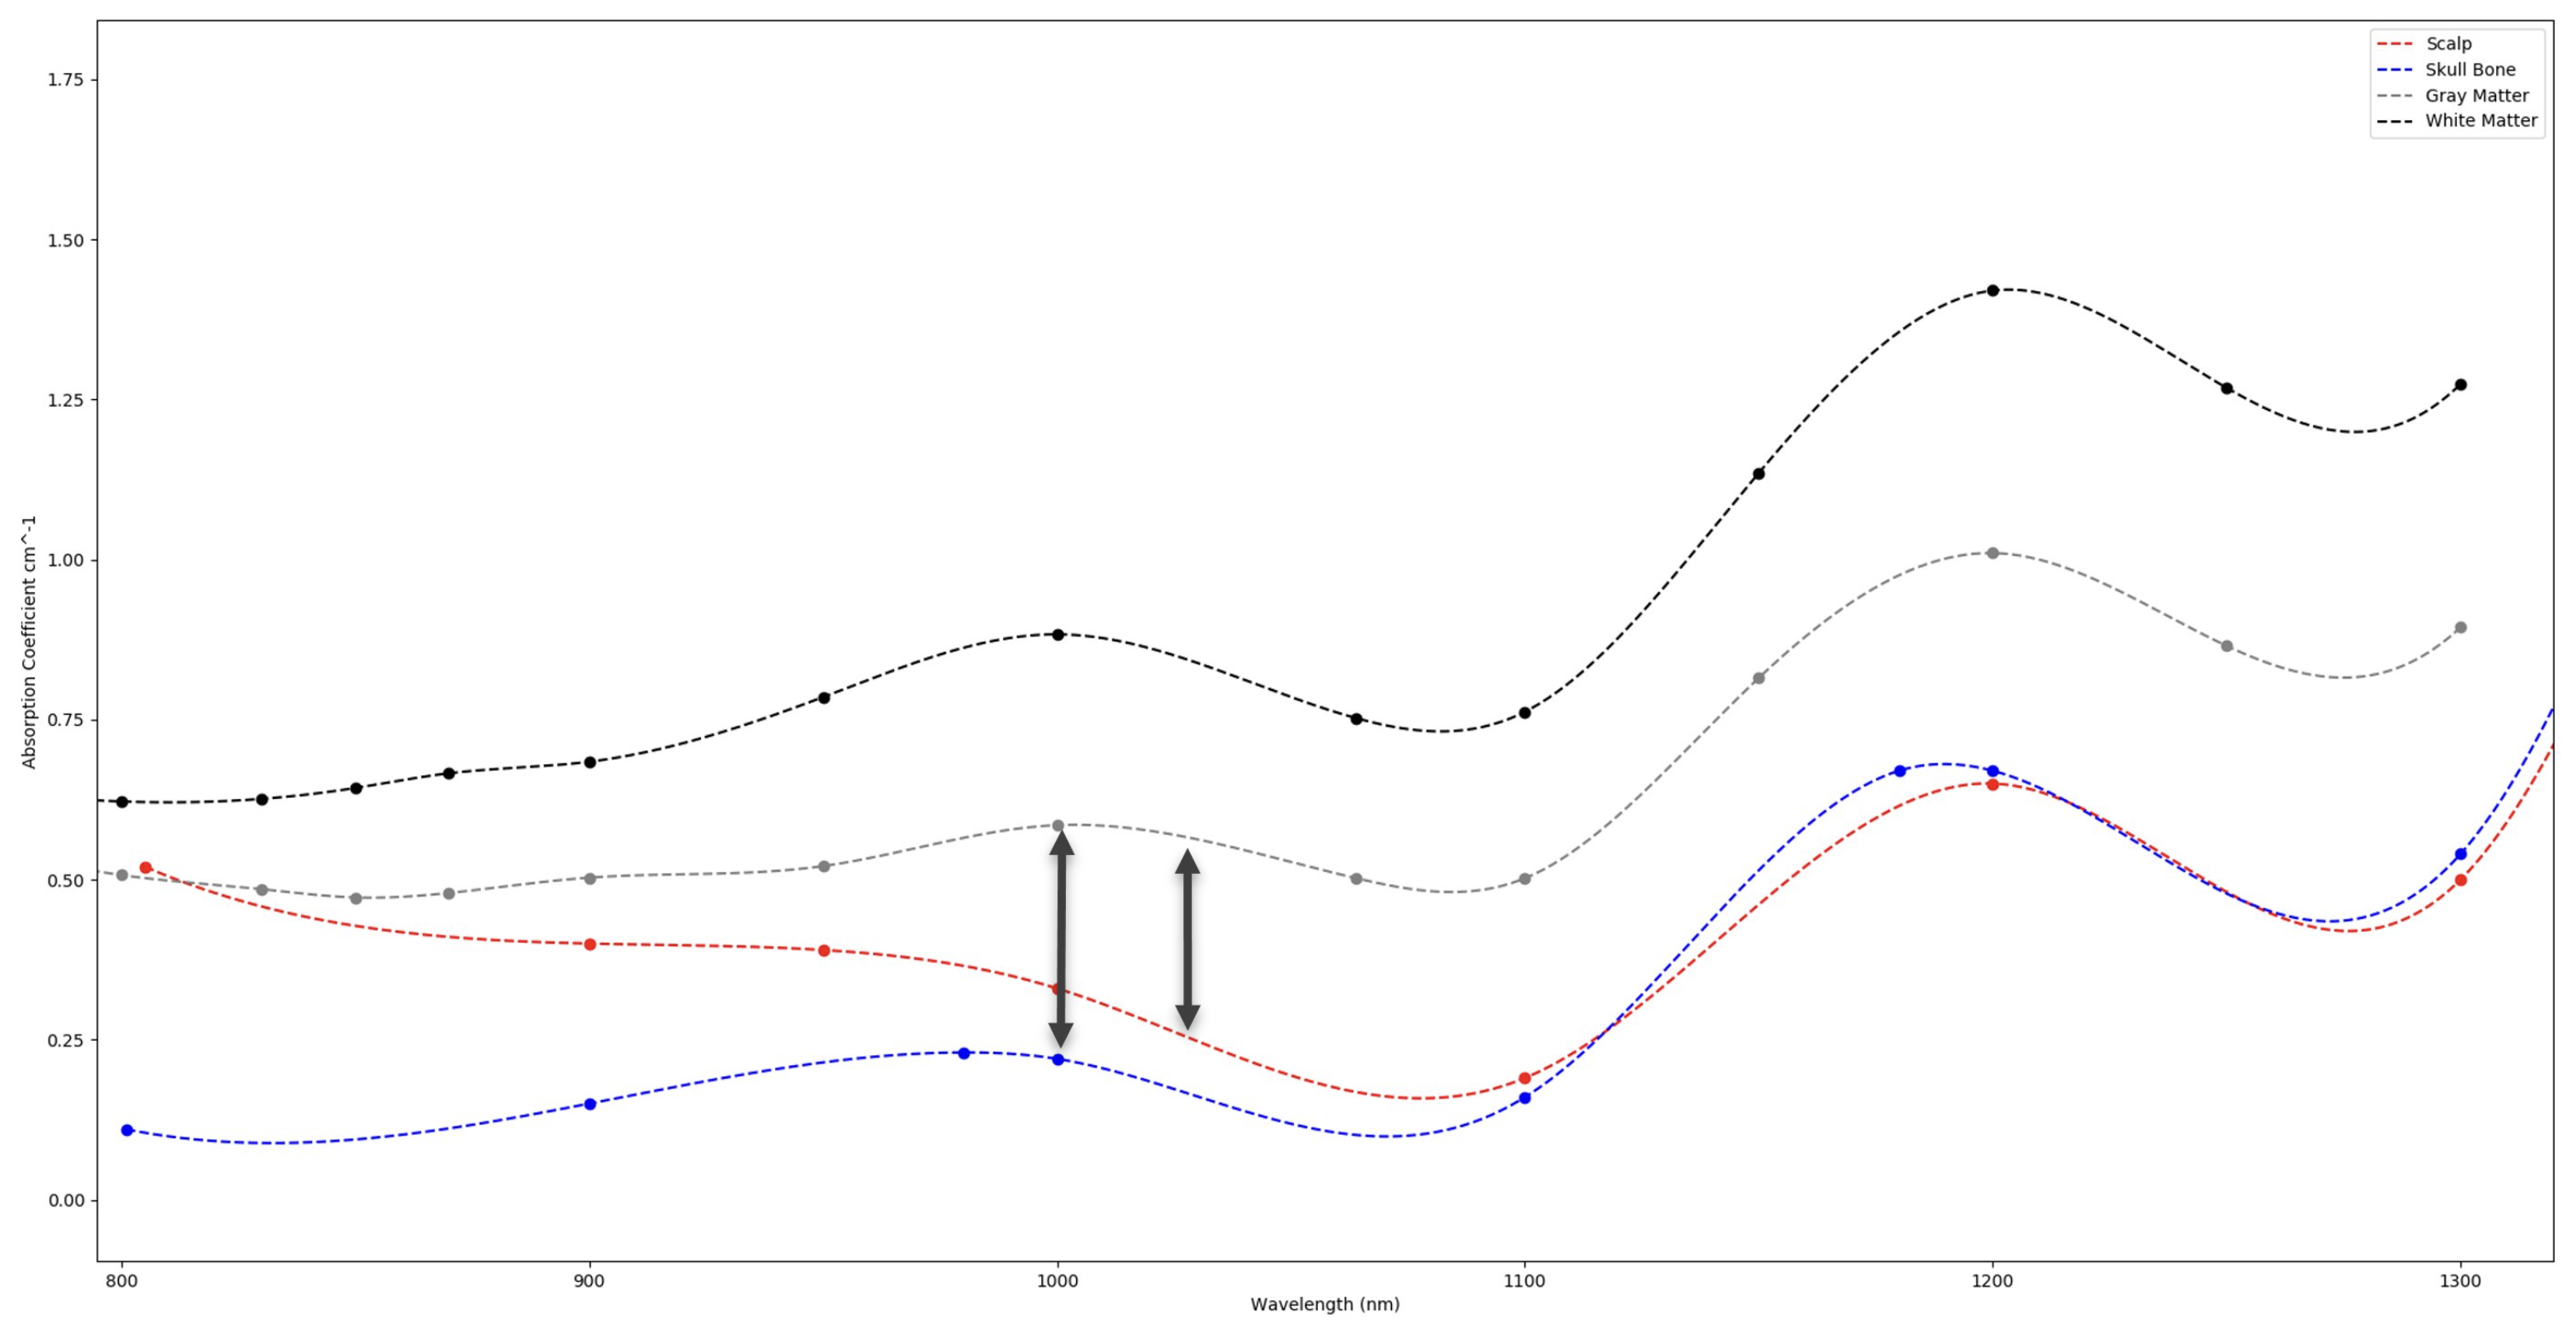
\includegraphics[width=\columnwidth]
    {Figures/OverlapDemonstration.png}}
    \caption{\label{fig:Overlap} Vertical Offset between different structures used for extrapolation process}
\end{figure}
In this study, Python programming language was used to process the absorption coefficient data and calculate the vertical offset values. 
The following equations were used to perform the extrapolation:
\begin{equation}
    \label{eq:GMextrapolate}
    \mu_{\text{GM,extrapolated}}(\lambda) = \mu_{\text{Skull,known}}(\lambda) + \text{AvgOffsetGM}
\end{equation}
\begin{equation}
    \label{eq:WMextrapolate}
    \mu_{\text{WM,extrapolated}}(\lambda) = \mu_{\text{WM,known}}(\lambda) + \text{AvgOffsetWM}
\end{equation}

To ensure accuracy and account for variations, this process of calculating vertical offsets and performing extrapolation is repeated for 
multiple data points within the overlapping region.

Figure \ref{fig:Extrapolation} visualizes the results of the extrapolation process.  These figures, generated using Python, provide a graphical representation of the 
extrapolation results and aid in understanding the estimated optical coefficients of the GM and WM layers at the wavelength of interest.
\begin{figure}[htb]
    \center{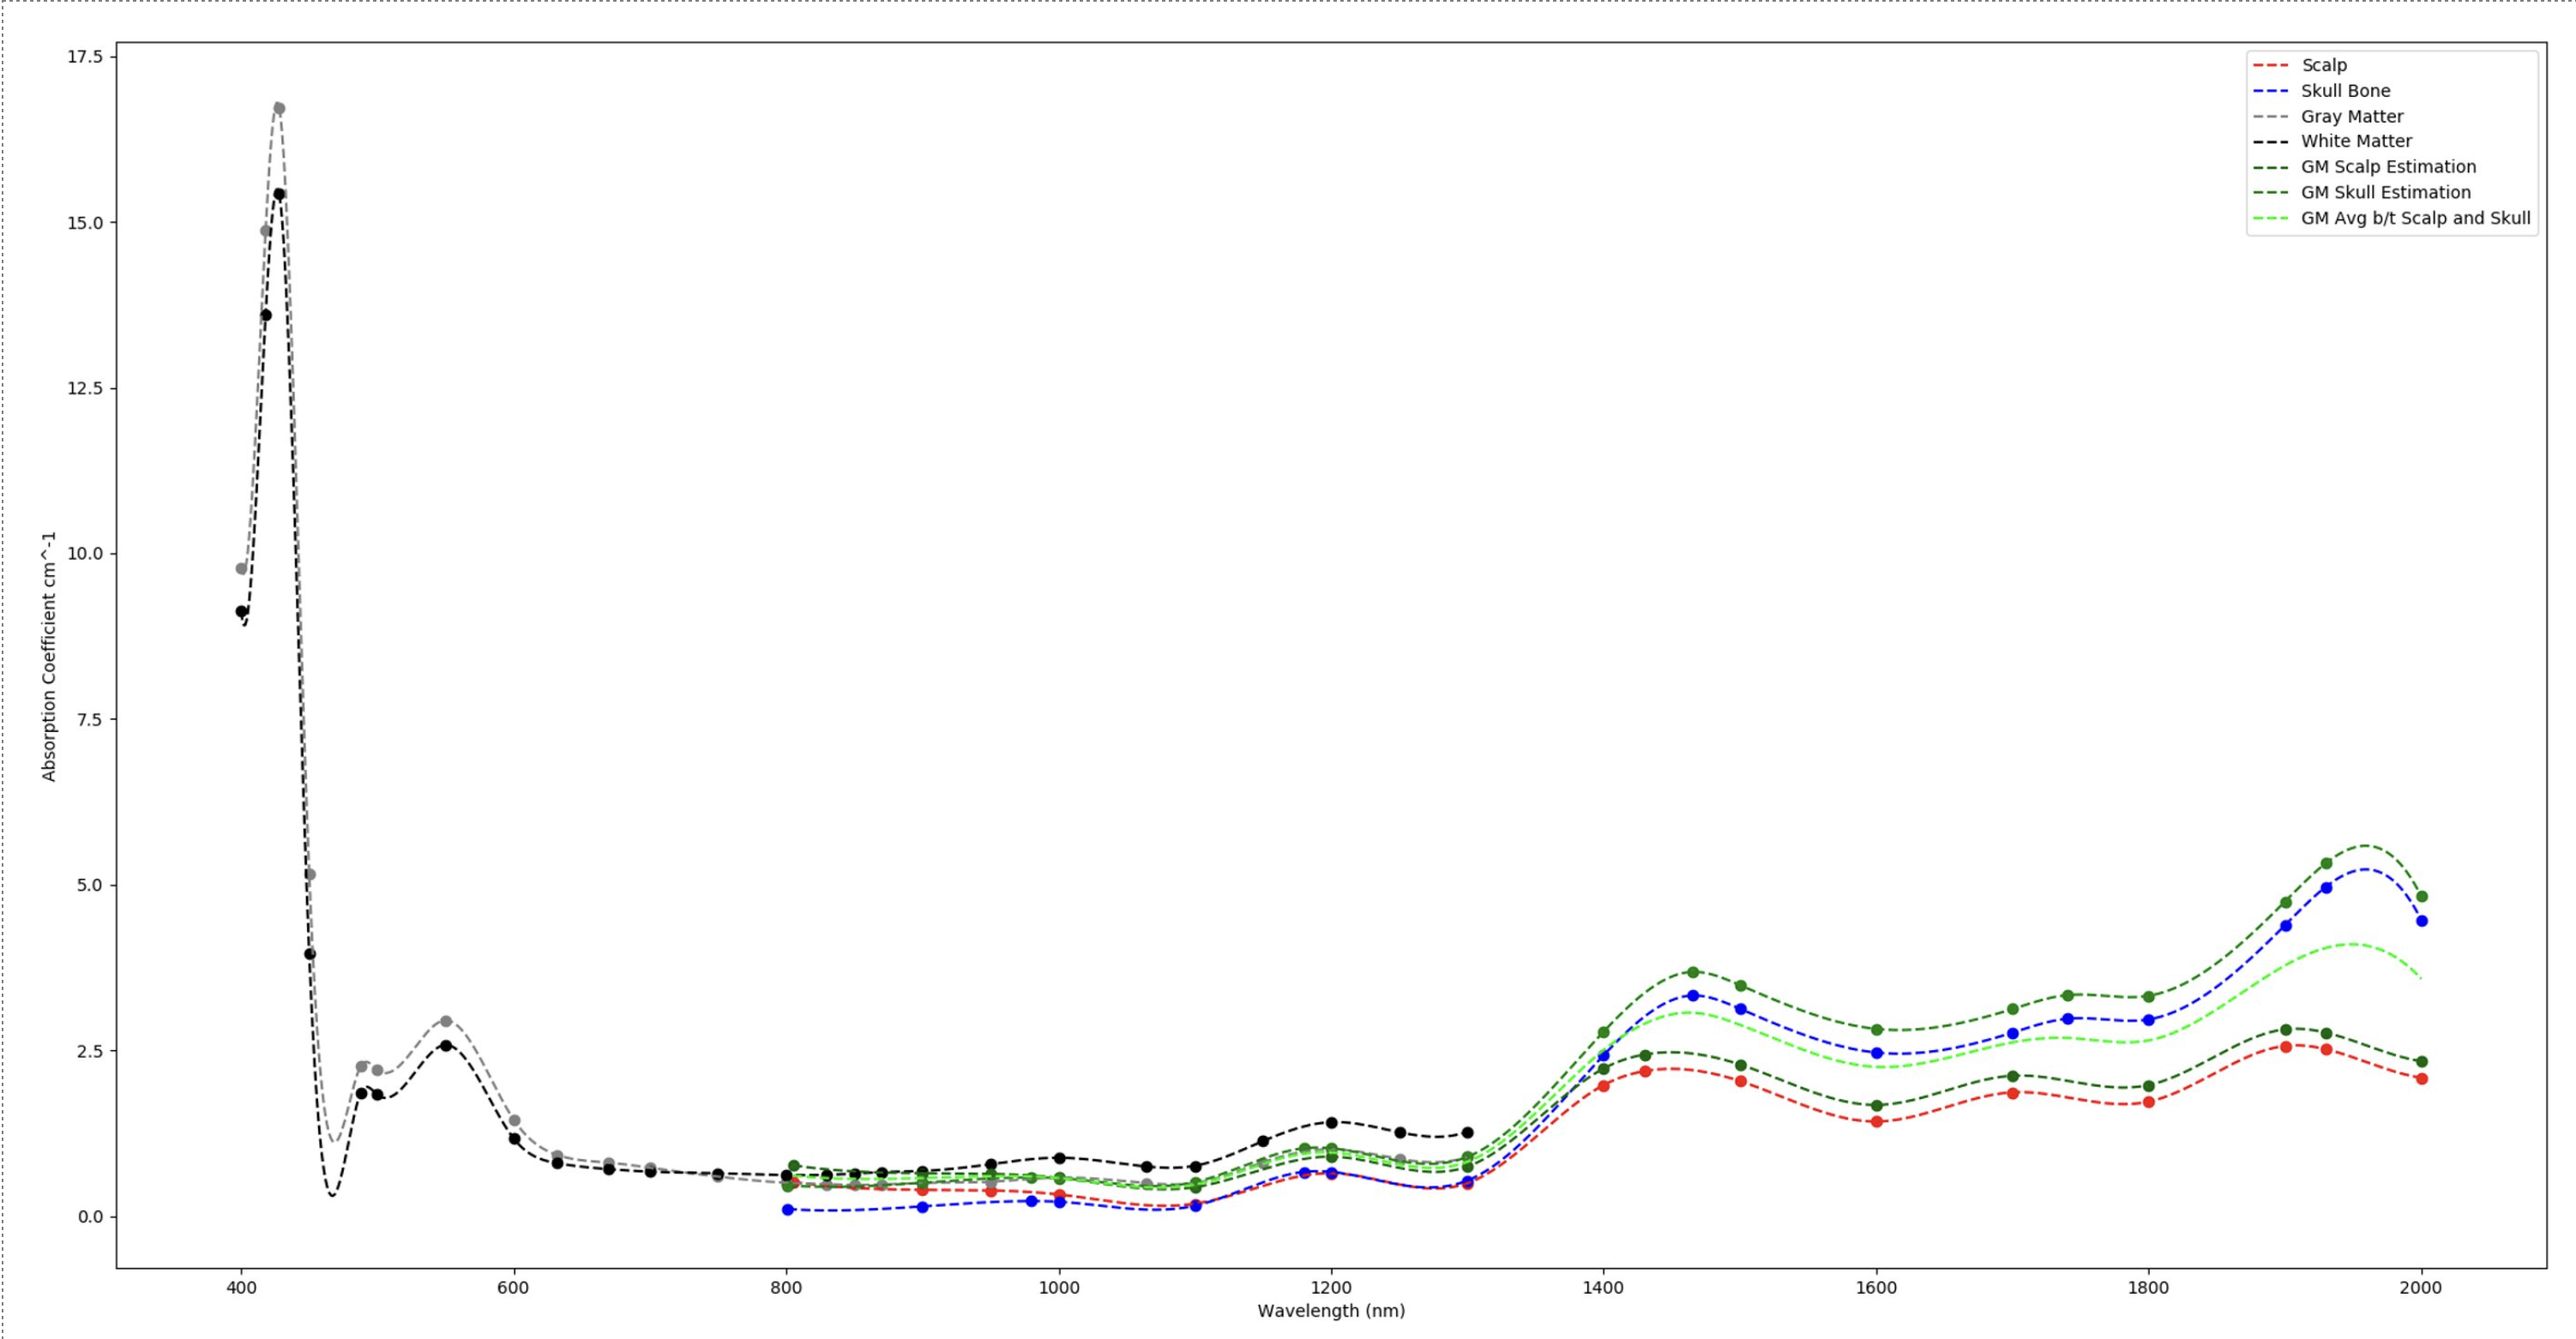
\includegraphics[width=\columnwidth]
    {Figures/ExtrapolationGraph.png}}
    \caption{\label{fig:Extrapolation} Completed Extrapolation Graph}
\end{figure}

\subsection{Simulation using MCX}
MCX, a Monte Carlo simulation tool \cite{b6}, is employed for visualizing the optical intensity and behavior of a laser source within the head and brain tissue. 
It models the photon dispersion in biological tissue using optical coefficients obtained from experimental data or approximations, as in the case of SWING. 
MCX creates a mesh model of the human brain using an accumulation of MRI images, incorporating layers such as scalp, skull, Cerebral Spinal Fluid (CSF), GM, WM, 
and air bubbles. Thickness variations in the layers are specified using thinning or thickening operators. To create the simulation, the optical coefficients, 
particularly the absorption and scattering coefficients, are input into the MCX software. This allows for the simulation of photon absorption and scattering as 
light passes through the brain tissue, enabling visualization of beam intensity at different points in the brain. Additionally, SWING utilizes the software to 
investigate various aspects of photon dispersion. This includes studying the impact of different tissue layers on beam intensity and exploring the effects of 
laser parameters such as wavelength, illumination area size, and the number of incident photons on the phantom. The differences between absorption coefficients at 
1550 nm compared to other wavelength be observed and noted in the figures, and this model can be utilized for experimental data validation.

\section{Results}
\label{sec:results}
Table~\ref{CoefficientTable} displays the estimated absorption and scattering coefficients for each of the biological tissue 
layers as well as each wavelength. These values were calculated using the interpolation-extrapolation method detailed in 
Section~\ref{sec:methods}. 
\begin{table}[hbt!]
    \centering
    \caption{Estimated Optical Coefficients}
    \label{CoefficientTable}
    \setlength{\tabcolsep}{3pt}
    \renewcommand{\arraystretch}{1.5}
    \resizebox{\columnwidth}{!}{%
    \begin{tabular}{|L{45pt}|L{55pt}|C{80pt}|C{80pt}|}
    \hline
    Tissue Type & Wavelength, nm & Absorption Coefficient $\mu_{a}$, cm$^{-1}$ &  Scattering Coefficient $\mu_{s}^{'}$, cm$^{-1}$ \\
    \hline
    Scalp & 810 & 0.505 & 14.145 \\
    &       980 & 0.365 & 16.714 \\
    &       1064 & 0.168 & 17.029 \\
    &       1550 & 1.649 & 14.578 \\
    \hline
    Skull & 810 & 0.099 & 19.248 \\
    &       980 & 0.230 & 17.380 \\
    &       1064 & 0.101 & 16.180 \\
    &       1550 & 2.715 & 15.543 \\
    \hline
    Gray Matter & 810 & [0.455,0.605,0.744] & [3.896,6.030,8.211] \\
    &       980 & [0.586,0.601,0.610] & [6.343,6.380,6.444] \\
    &       1064 & [0.413,0.438,0.457] & [5.143,5.938,6.740] \\
    &       1550 & [1.870,2.485,3.071] & [4.246,4.393,4.506] \\
    \hline
    White Matter & 810 & [0.737,0.888,1.027] & [24.237,26.403,28.617] \\
    &       980 & [0.868,0.883,0.893] & [26.749,26.753,26.785] \\
    &       1064 & [0.696,0.720,0.739] & [25.549,26.311,27.081] \\
    &       1550 & [2.153,2.767,3.353] & [24.587,24.767,24.911] \\
    \hline
    \end{tabular}%
    }
    \label{tab1}
\end{table}

To determine the reliability of this prediction method, SWING used the Python library scikit-learn\cite{b7} 
to calculate the $R^2$ value when predicting known data. Scitkit-learn calculated the $R^2$ value, as referenced in \cite{b7}, as follows:
first, the residual sum of squares, $SS_{res}$,
\begin{equation}
    \label{eq:ResidSumSquares}
    SS_{res} = \sum_{i}{(y_i-f_i)^2}
\end{equation}
where $y_i$ is the known variable value, and $f_i$ is the predicted variable value.
Next, the total sum of squares, $SS_{tot}$,
\begin{equation}
    \label{eq:TotSumSquares}
    SS_{tot} = \sum_{i}{(y_i-\overline{y})^2}
\end{equation}
where $\overline{y}$ is the mean of the known data.
\begin{equation}
    \label{eq:CoeffDeterm}
    R^2 = 1 - \frac{SS_{res}}{SS_{tot}}
\end{equation}

This $R^2$ value was calculated as 0.4980, indicating that 49.80\% of the variability in the unknown coefficients is 
explained by SWING's prediction model.

\begin{figure}[hbt!]
    \begin{subfigure}{.475\linewidth}
      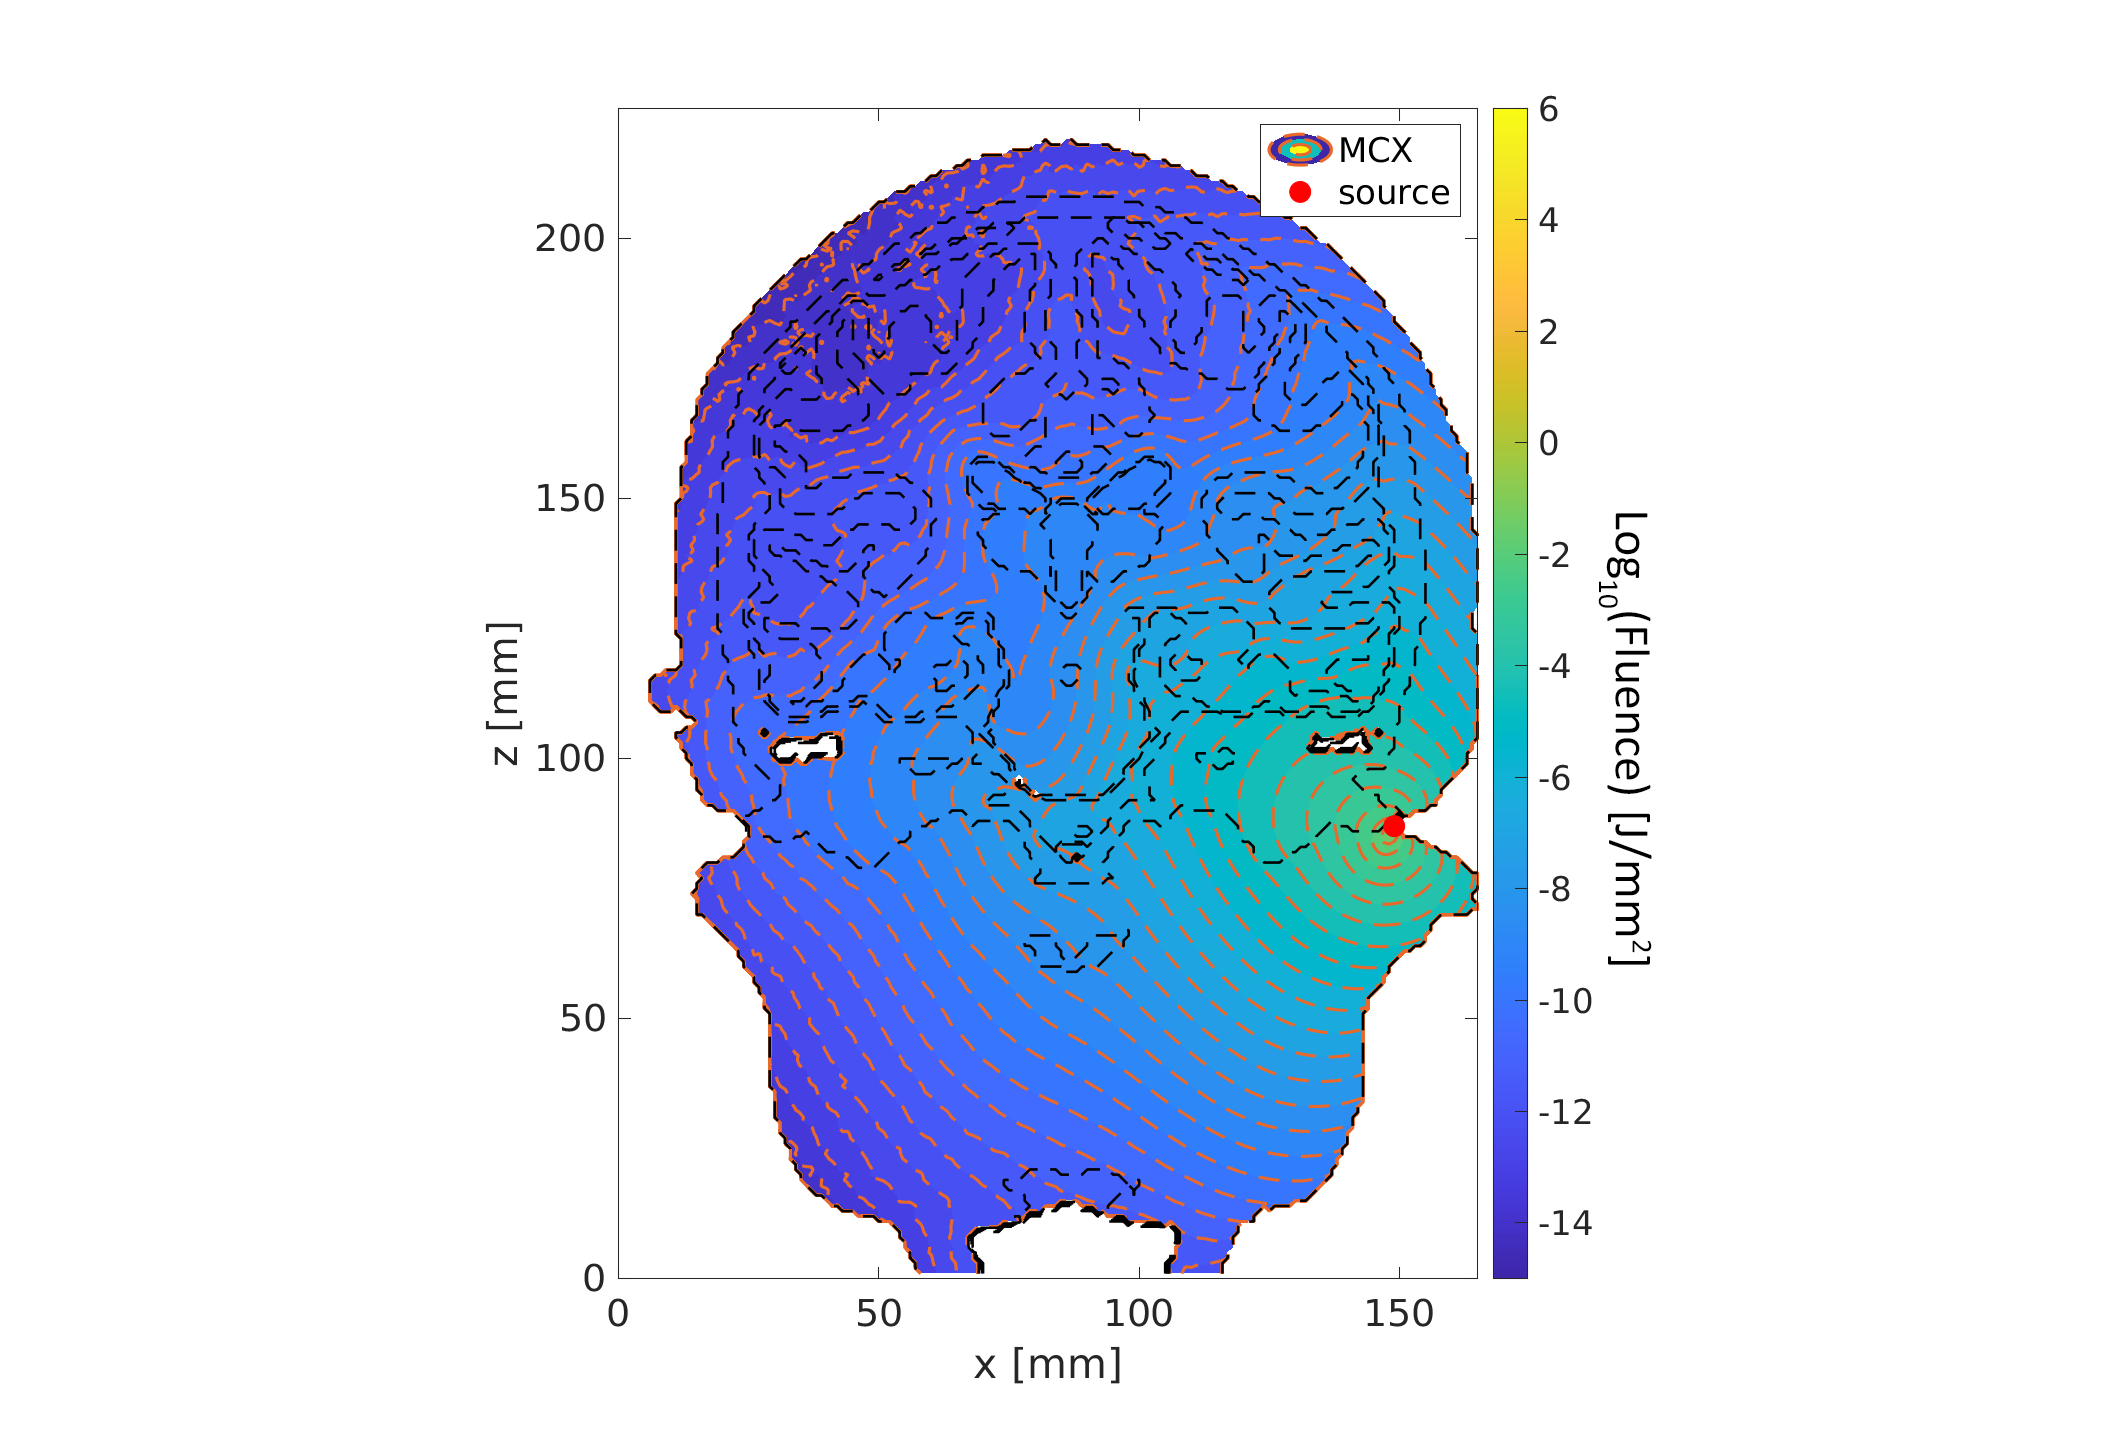
\includegraphics[width=\linewidth]{Figures/Fluence_Distribution_810nm_Cochlear.png}
      \caption{810 nm Fluence Distribution}
      \label{fig:810Fluence}
    \end{subfigure}
    \hfill
    \begin{subfigure}{.5\linewidth}
      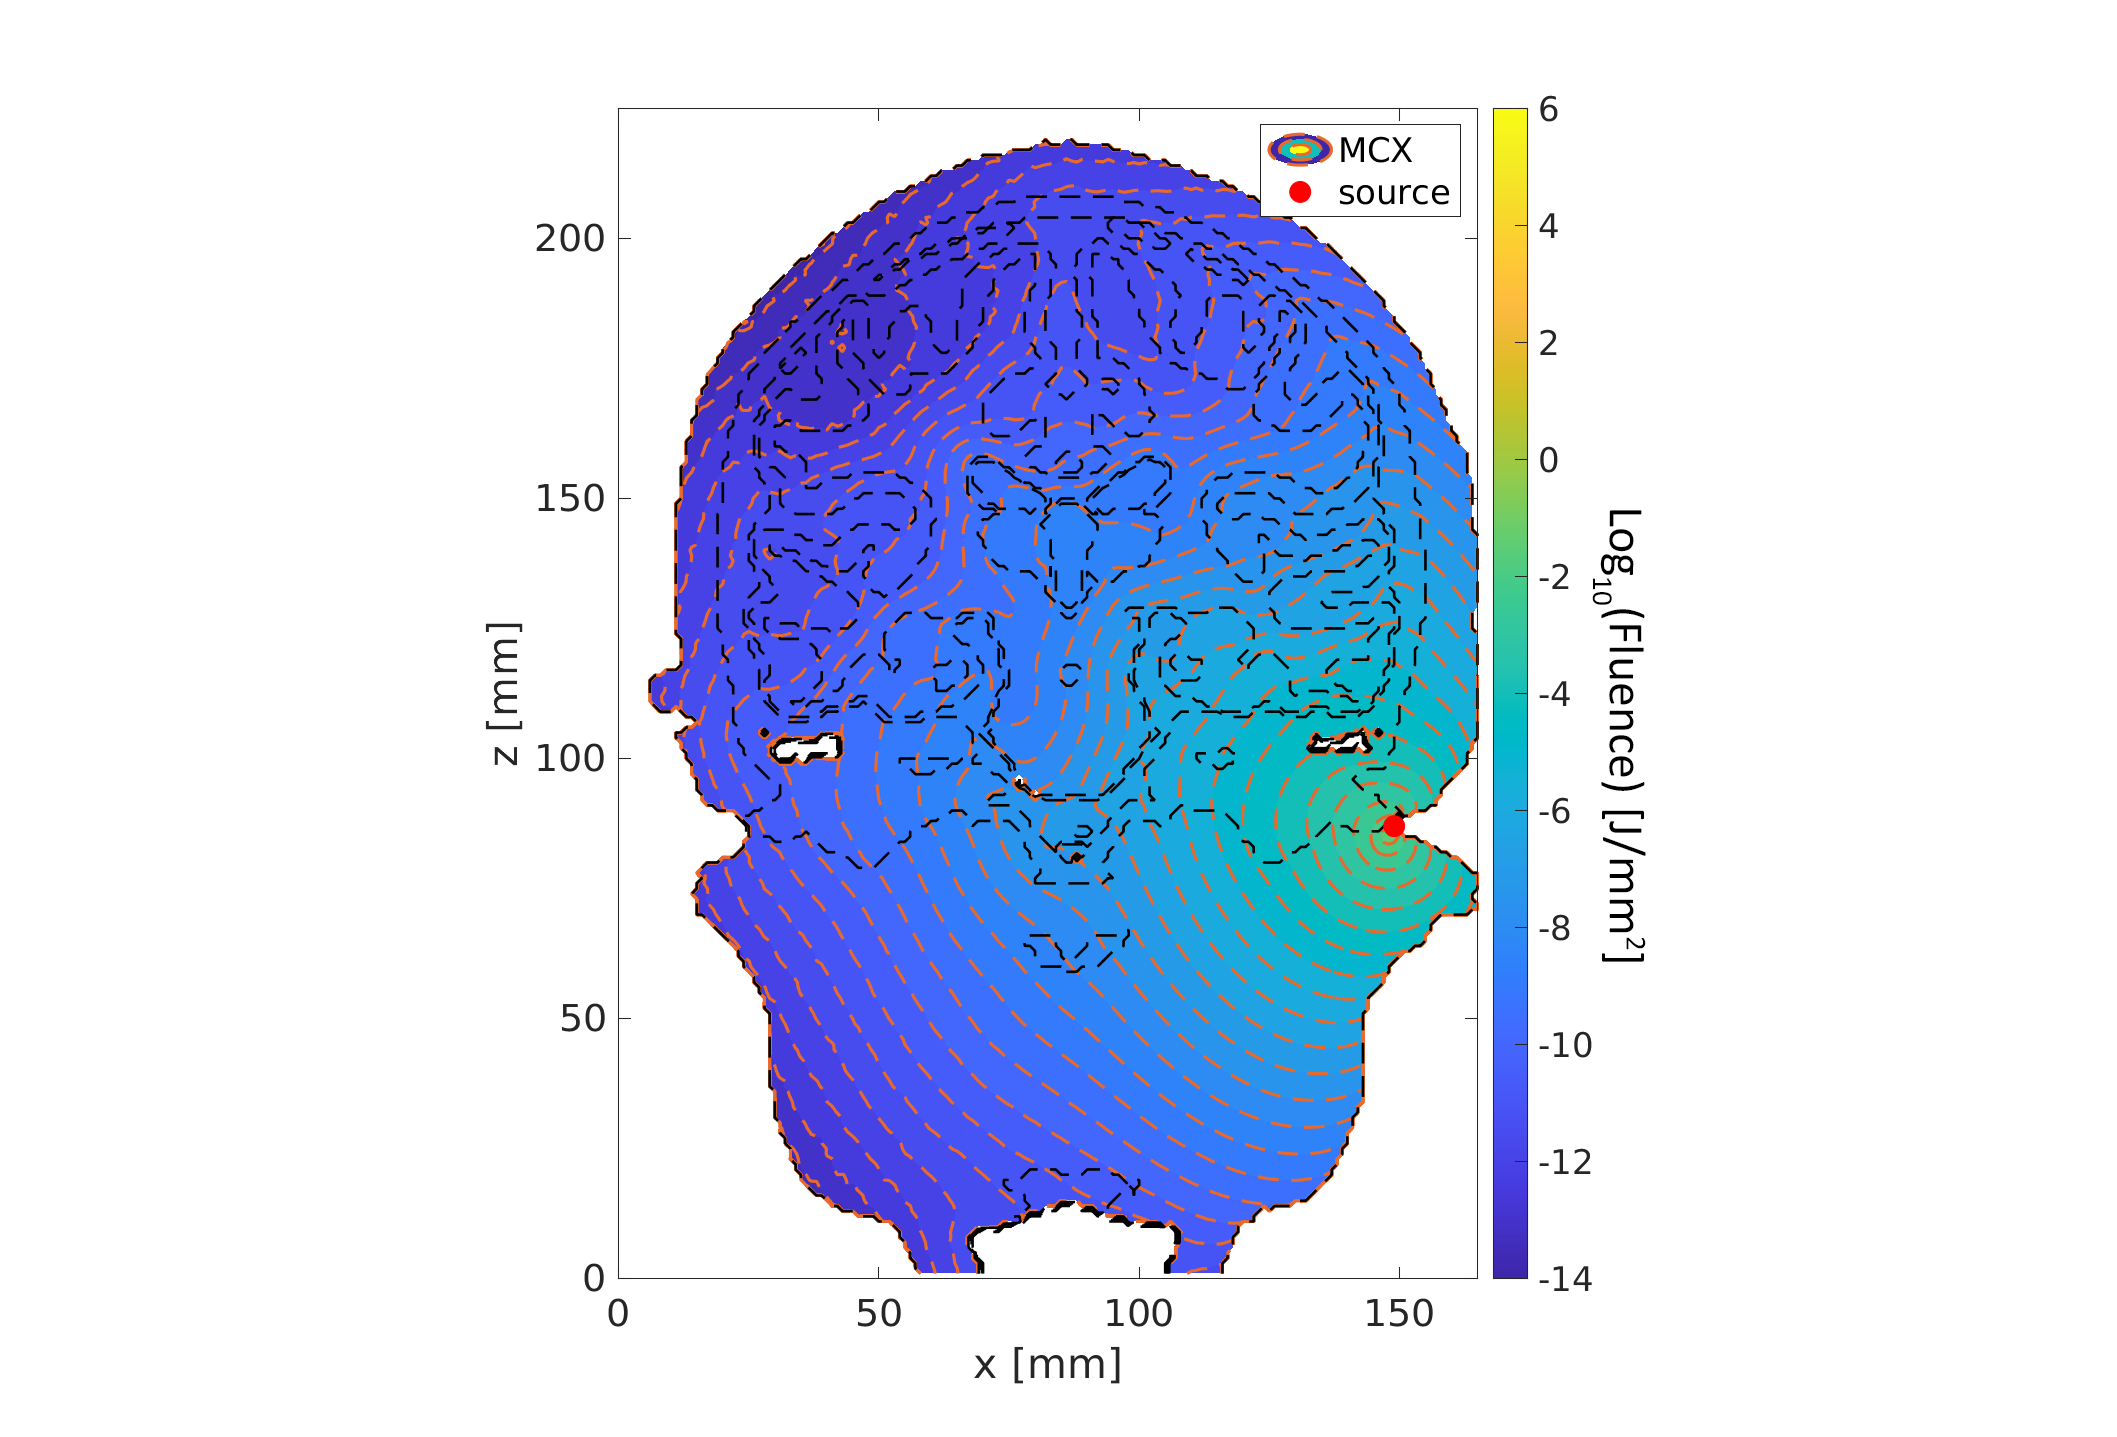
\includegraphics[width=\linewidth]{Figures/Fluence_Distribution_980nm_Cochlear.png}
      \caption{980 nm Fluence Distribution}
      \label{fig:980Fluence}
    \end{subfigure}
    
    \medskip
    \begin{subfigure}{.475\linewidth}
      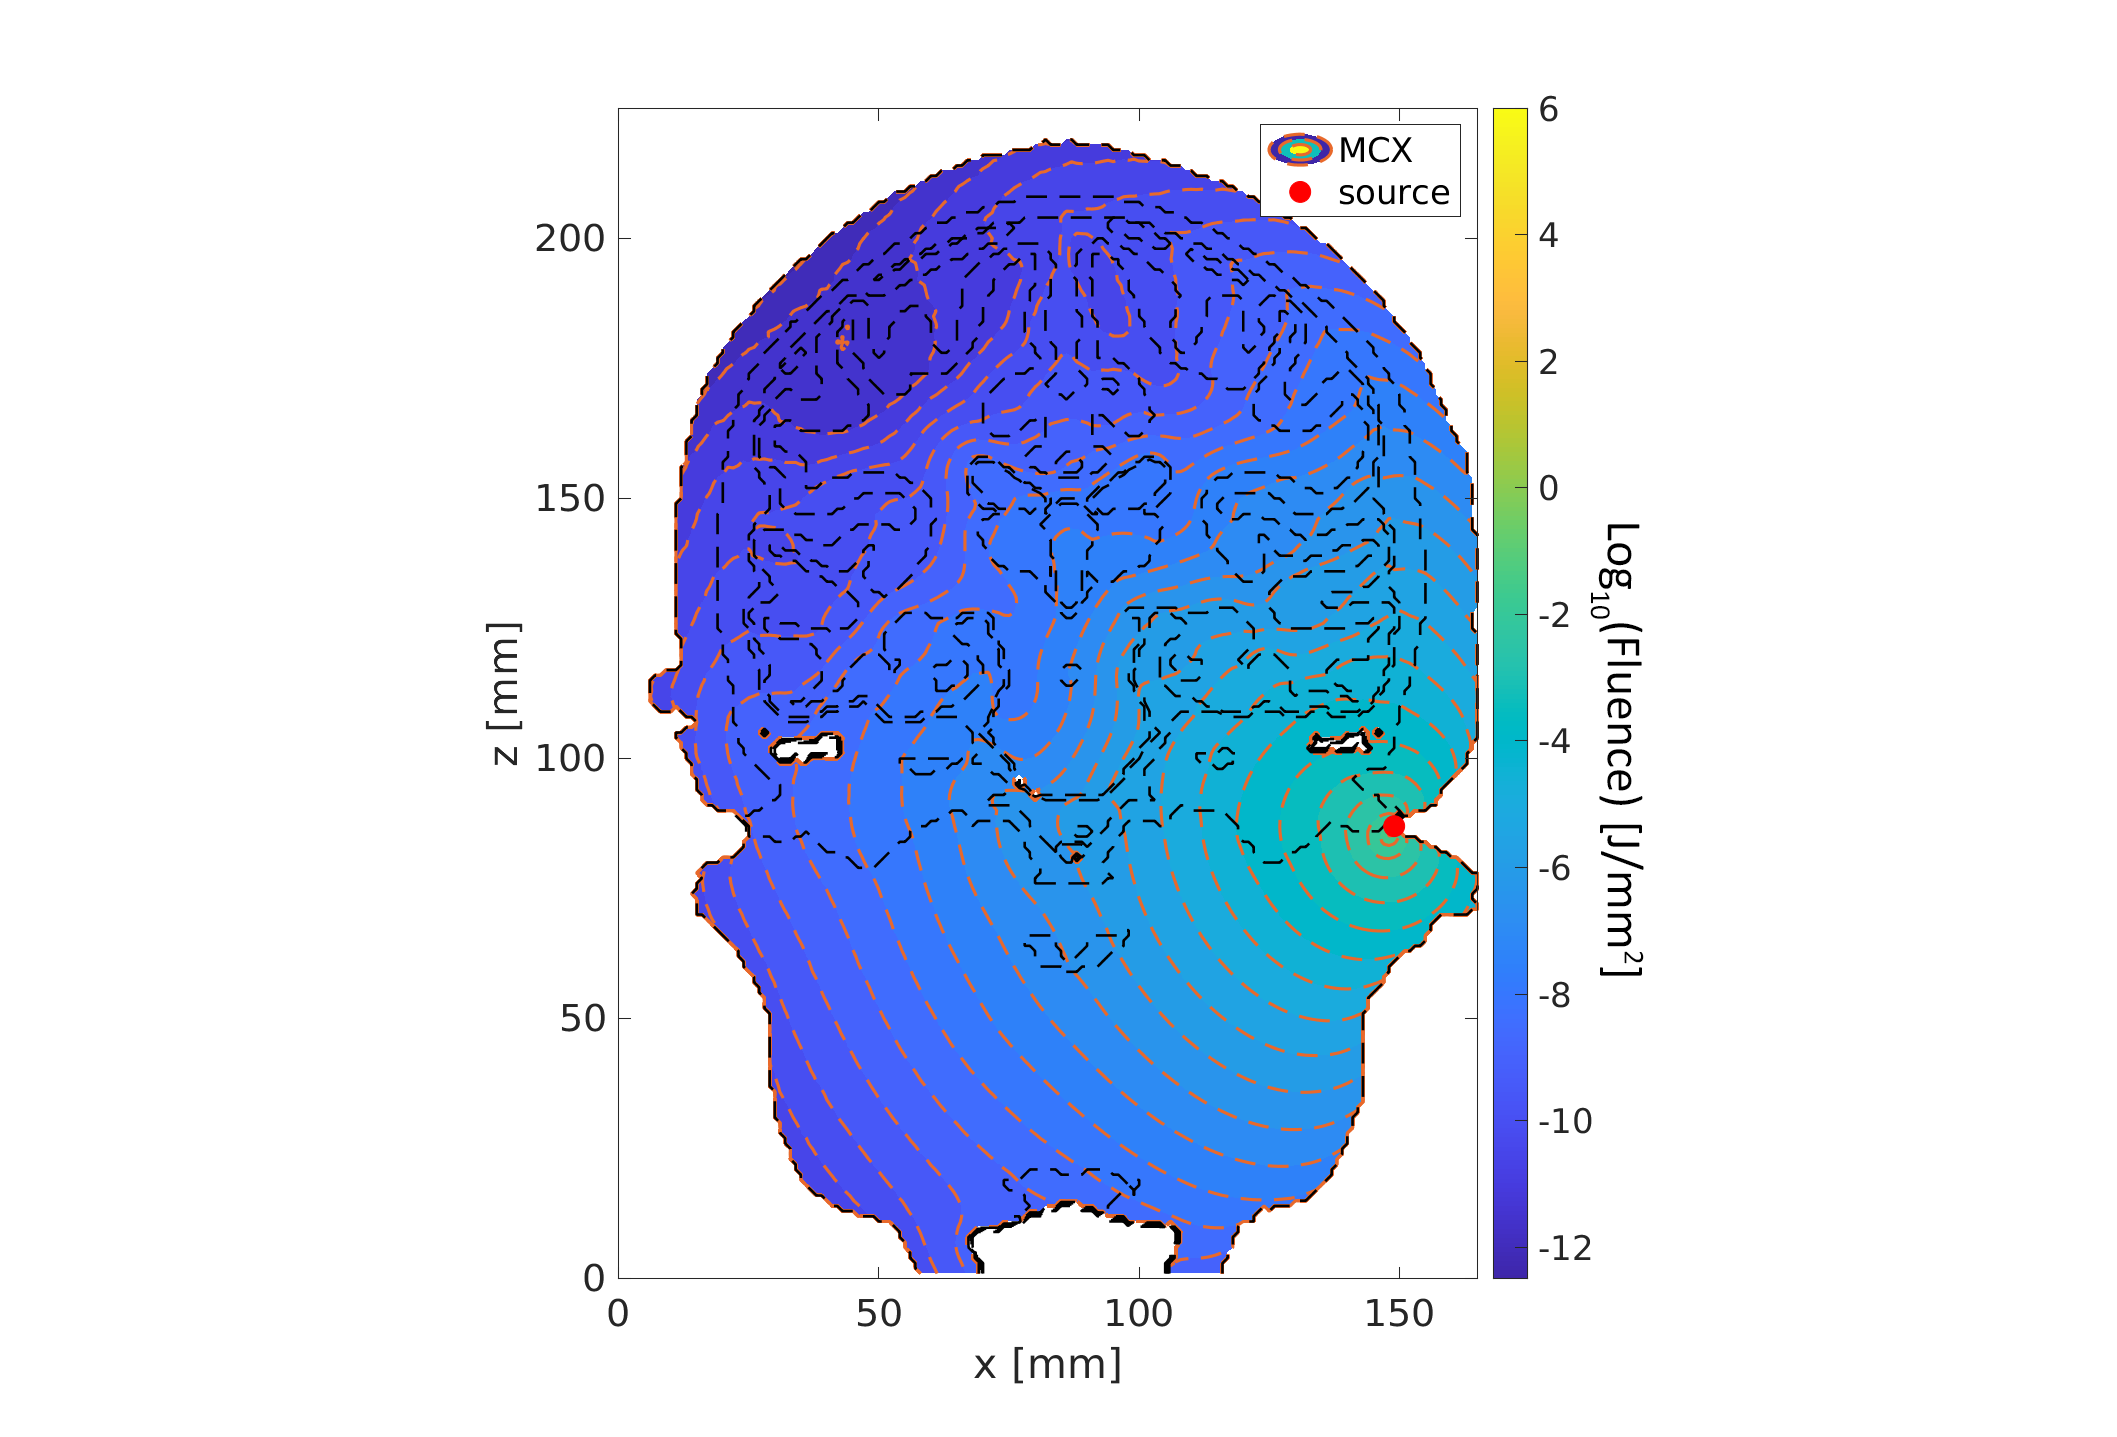
\includegraphics[width=\linewidth]{Figures/Fluence_Distribution_1064nm_Cochlear.png}
      \caption{1064 nm Fluence Distribution}
      \label{fig:1064Fluence}
    \end{subfigure}
    \hfill
    \begin{subfigure}{.5\linewidth}
      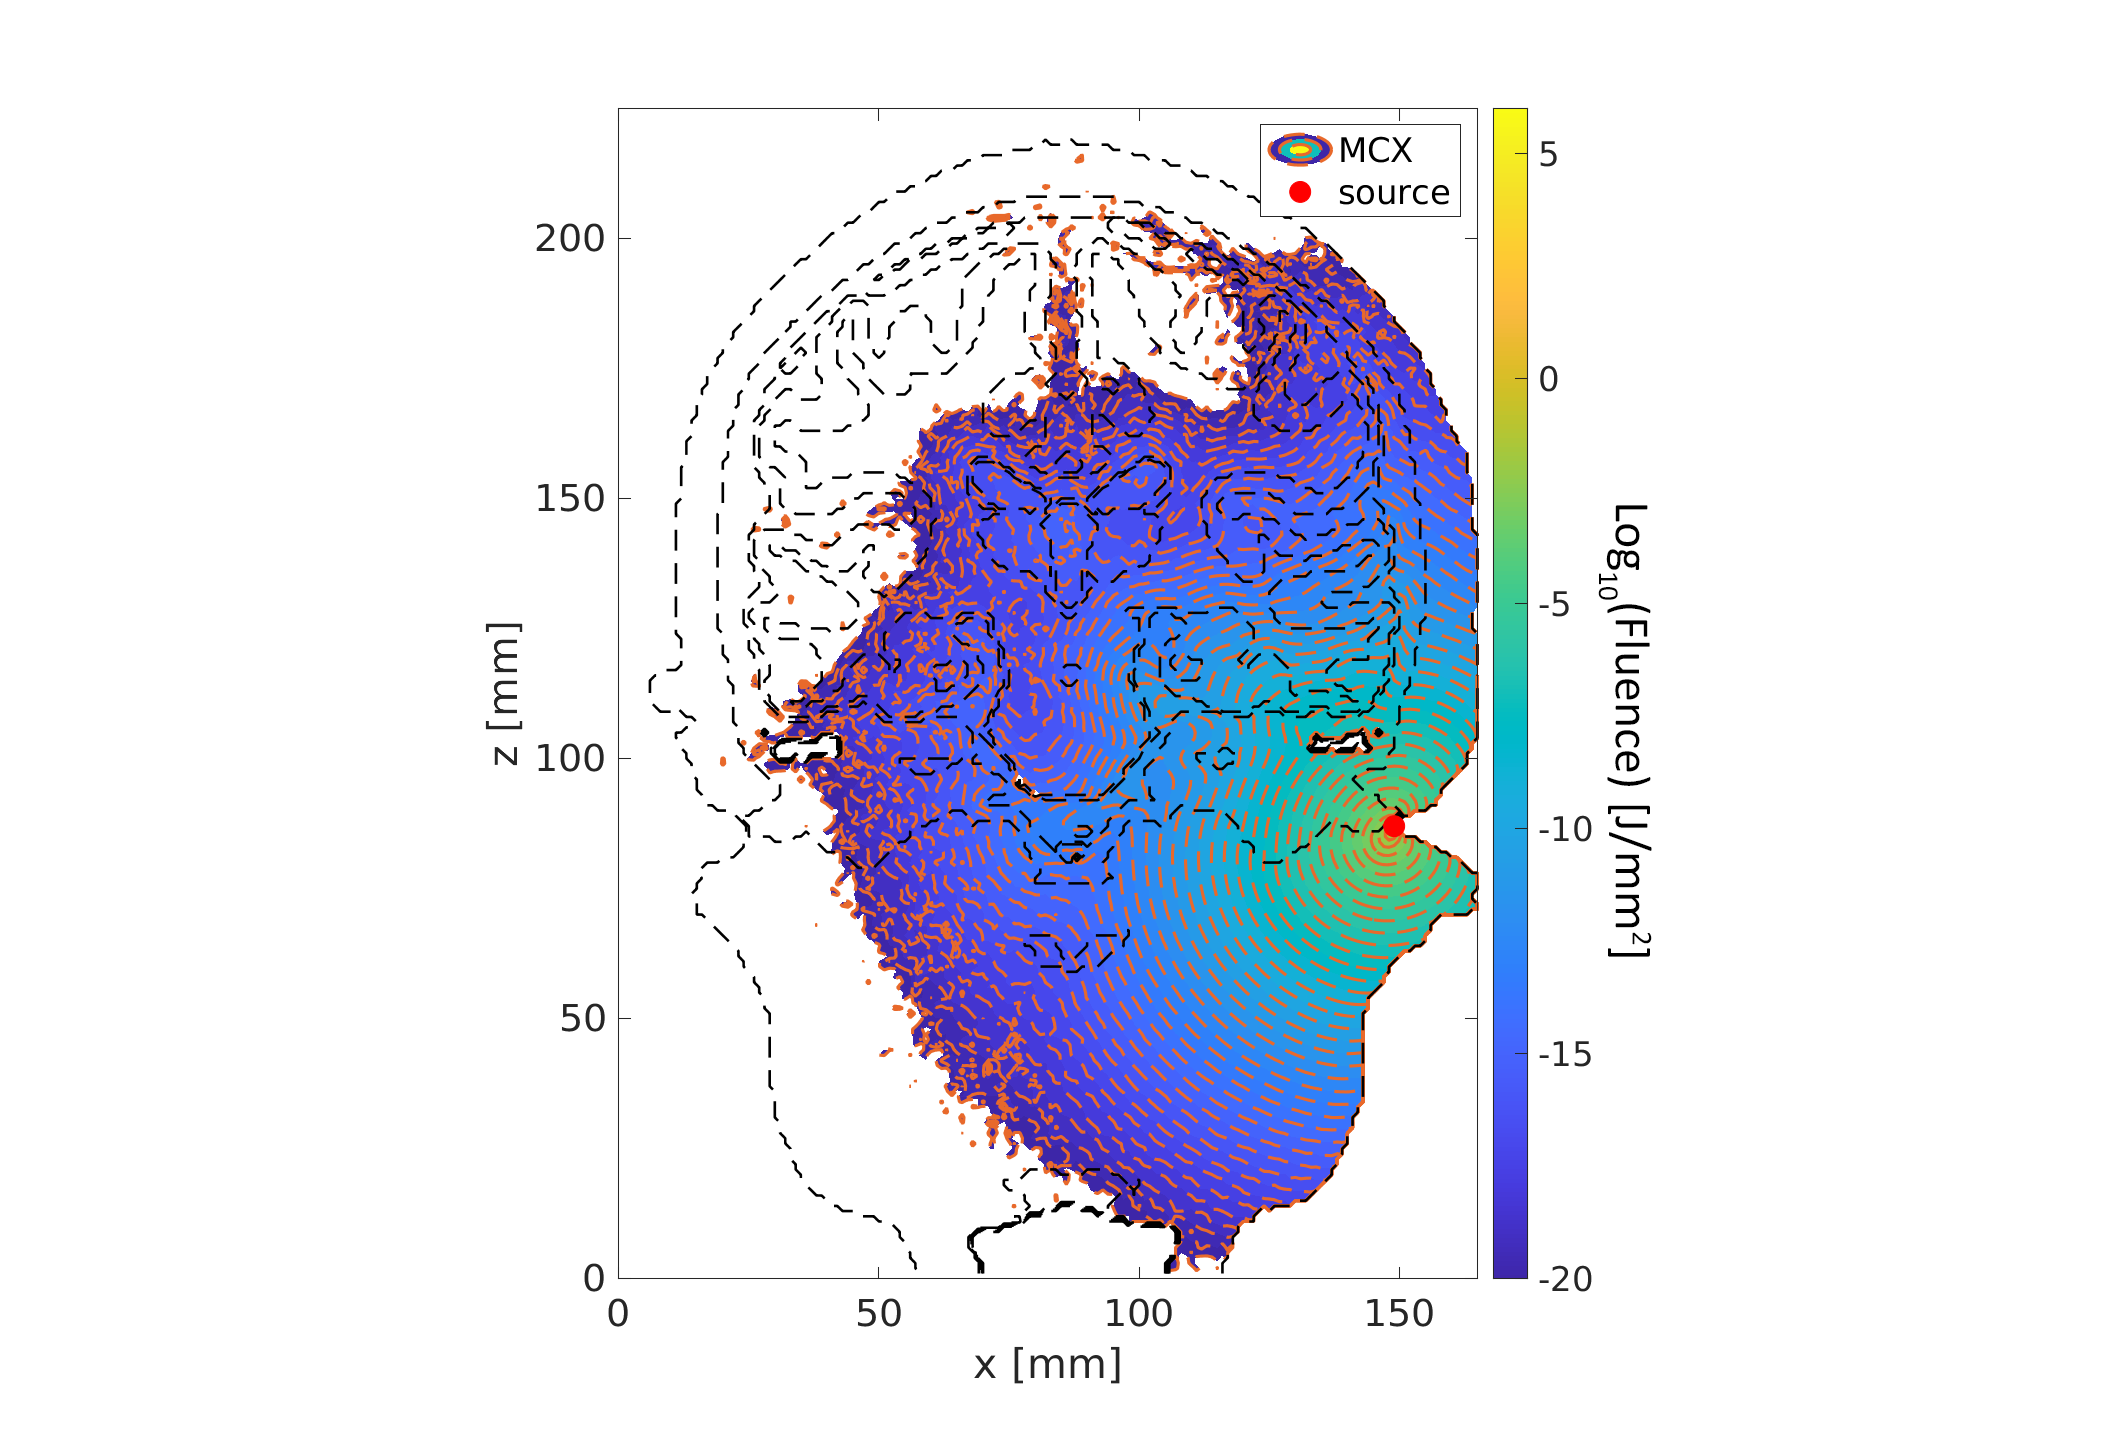
\includegraphics[width=\linewidth]{Figures/Fluence_Distribution_1550nm_Cochlear.png}
      \caption{1550 nm Fluence Distribution}
      \label{fig:1550Fluence}
    \end{subfigure}
    
    \caption{Cochlear Fluence Distribution 810 nm - 1550 nm}
    \label{fig:fluence_quarters}
\end{figure}

Fig. \ref{fig:fluence_quarters} shows the MCX simulations at the wavelengths 810, 980, 1064, and 1550 nm. Each simulation uses the same number
of photons, \num{1.0e11}, and duration, \SI{100}{\milli\second}. The variables controlling the coverage of the light are 
$\mu_{a}$, and $\mu_{s}^{'}$ found in Table \ref{CoefficientTable}. These simulations use the cochlear pathway for providing laser stimulation, the additional 
positions considered are: the CZ position using the 10-20 system for electroencephalography (EEG), 45-degree position which sits at a 45-degree angle between the 
cochlear and CZ positions, and the intranasal position. These simulations can be found in Appendices \ref{app:810Simulations}, \ref{app:980Simulations}, 
\ref{app:1064Simulations}, and \ref{app:1550Simulations}

SWING's considerations for an effective wavelength for treatment are: maximum achievable depth from the photon injection point, energy level at the points of interest 
(dorsal striatum, ventral striatum, and motor cortex), and minimizing risk of unwanted side effects such as stimulation to other portions 
of the brain, or damage to tissue. With these considerations in mind, 1550 nm was chosen as the best simulated wavelength. 1550 nm light 
provides a depth sufficient for stimulating the striatum and motor cortex, and due to its lower energy compared to 810, 980, and 1064 nm has a 
lower risk of causing tissue damage. While the former consideration is visually observable, the latter consideration is demonstrated by 
Planck's equation for calculating the energy of a photon:
\begin{equation}
    \label{eq:PhotonEnergy}
    E = \frac{hc}{\lambda}
\end{equation}
where $h$ is Planck's constant: \SI{6.626e-34}{\joule\second}, $c$ is the velocity of light: \SI{3.0e8}{\meter\per\second}, and $\lambda$ is 
the wavelength of the photon, e.g. \SI{1550e-9}{\meter}. 

\begin{equation}
    \label{eq:810Energy}
    E = \frac{\num{6.626e-34}\cdot\num{3.0e8}}{\num{810e-9}} = \SI{2.454e-19}{\joule}
\end{equation}

\begin{equation}
    \label{eq:980Energy}
    E = \frac{\num{6.626e-34}\cdot\num{3.0e8}}{\num{980e-9}} = \SI{2.028e-19}{\joule}
\end{equation}

\begin{equation}
    \label{eq:1064Energy}
    E = \frac{\num{6.626e-34}\cdot\num{3.0e8}}{\num{1064e-9}} = \SI{1.868e-19}{\joule}
\end{equation}

\begin{equation}
    \label{eq:1550Energy}
    E = \frac{\num{6.626e-34}\cdot\num{3.0e8}}{\num{1550e-9}} = \SI{1.282e-19}{\joule}
\end{equation}
Eq. \eqref{eq:1550Energy} shows that a 1550 nm photon has an energy of \SI{1.282e-19}{\joule}, which is lower than that of 810 nm, 980 nm, and 1064 nm. However, 
the energy of one 1550 nm photon is not enough to activate a neuron or a group of neurons. The energy needed to activate a neuron considered by SWING as a 
necessary level for neuron stimulation is \SI{2.468e-7}{\joule} \cite{b8}. In order to achieve this energy level deep within the brain SWING simulated from 
\num{1.0e6} photons to \num{1.0e11} photons. Once SWING attempted to simulate \num{1.0e12} photons or more, the necessary time for one simulation to finish 
increased from taking 30 minutes for \num{1.0e11} to 4 hours or longer.

\begin{figure}[hbt!]
    \center{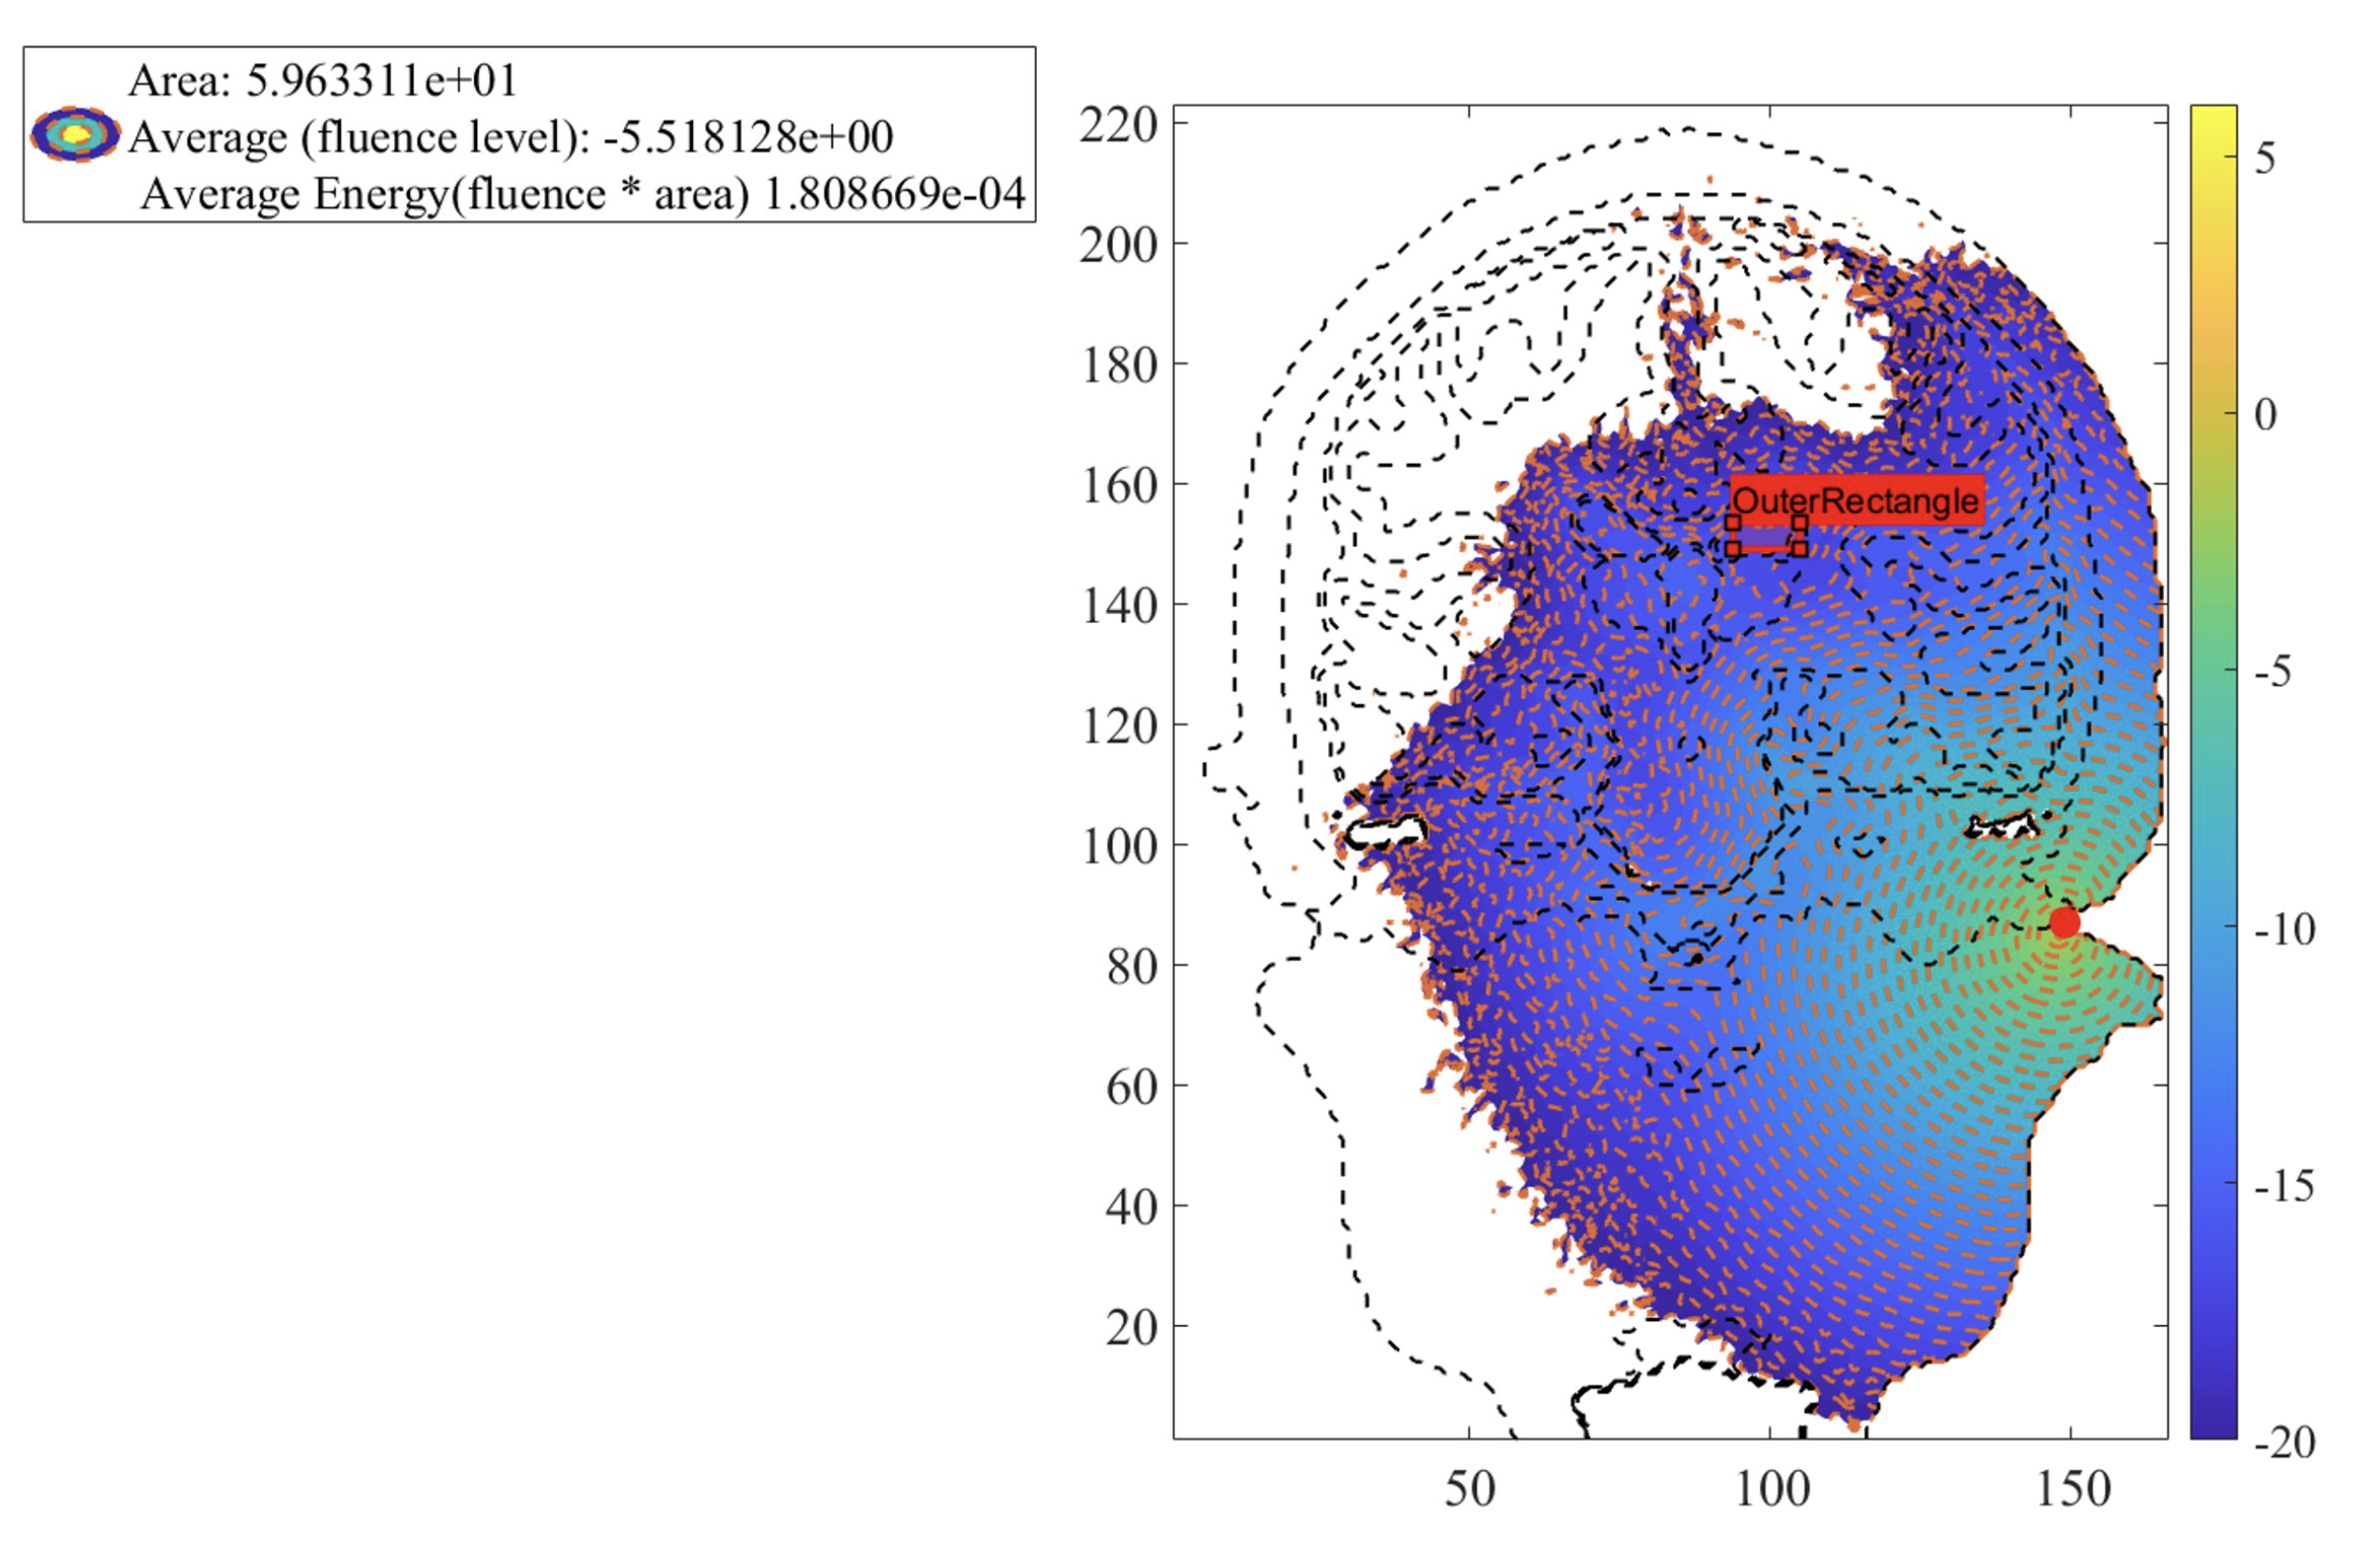
\includegraphics[width=\columnwidth]
    {Figures/Avg1550.png}}
    \caption{\label{fig:Avg1550} Average Energy and Fluence in the Striatum at 1550nm}
\end{figure}

The average energy in the striatum at 1550nm resulting from cochlear penetration, as shown in Fig. \ref{fig:Avg1550} is calculated to 
be \SI{1.801e-4}{\joule}. Achieving this energy level is significant as it surpasses the necessary \SI{2.468e-7}{\joule} to provide stimulation by an order of three. 
This excess energy could be decreased by lowering the output power of the injection laser in order to decrease the chance of unwanted neuron 
activation in other regions of the brain.

\section{Discussion}
\label{sec:next steps}
In this paper, SWING presented justification for further exploration of using photobiomodulation for non-invasive deep brain stimulation. While 
shorter wavelengths considered in this paper (810 nm, 980 nm, and 1064 nm) provided deep brain stimulation, they also provided large area stimulation. 
This result could lead to undesired activation of non-targeted portions of the brain. Through these simulations, SWING presented 1550 nm as a candidate for 
providing targeted deep brain stimulation. Specifically, SWING identified that 1550 nm light provides a platform for further development in targeted 
stimulation of the dorsal striatum, ventral striatum, and the motor cortex for treatment of diseases like Parkinson's, Alzheimer's, Dementia, and many others.

The nature of exploring novel techniques introduces limitations. Consideration of the empirical results is presented in the light of these limitations. One such
limitation is the lack of clinical trials or a physical optical phantom to provide validation for the data presented. Another limitation would be the acquisition
of biological tissue optical coefficients. SWING used an interpolation and extrapolation method to estimate the absorption and reduced scattering coefficients for
the gray matter and white matter based on empirically observed coefficients\cite{b5} for the scalp and skull. These limitations provide a basis for the
development of planning for future work. 

Future work on non-invasive optical stimulation would require a physical validation of the simulation results. 
One pathway for validation is through shooting a laser, with the same wavelengths used in MCX, through an optical phantom head and 
measuring the energy levels throughout the optical phantom. Additionally, as part of incorporating a physical validation to SWING's results
clinical trials, which would include the development of a wearable prototype for testing. Lastly, the use of additional functional MRI (fMRI) scans
for simulation would provide confidence in the expected photon fluence. These are the areas that the members of SWING identified as necessary for 
additional exploration.

\section{Conclusion}
\label{sec:conclusion}
The work presented by SWING represents a novel method for direct stimulation of neurons in the brain using 1550 nm light. This holds significant potential 
for the treatment of various diseases such as Parkinson's, Alzheimer's, and various mental afflictions. 
While invasive stimulation methods carry risks of exacerbating the condition or causing infections, SWING explored a non-invasive optical stimulation approach. 
With funding from the KIND Laboratory's Brain IMPACT project, and as part of the Electrical and Computer Engineering capstone sequence at The Ohio State University, 
SWING utilized a cubic extrapolation to approximate the optical coefficients of biological tissue up to and past 1550 nm. Through extensive simulations conducted on 
the Ohio State Supercomputer using MCX, non-invasive deep brain stimulation demonstrated feasibility at various wavelengths. Notably, 
the MCX results compel further investigation and testing of the 1550 nm wavelength as the most promising choice for future endeavors in this field. 

\section*{Acknowledgment}

\begin{thebibliography}{00}

\bibitem{b1} ``Novel Neuromodulation Techniques,`` in \emph{IEEE Pulse}, Aug. 2016. 
\url{https://www.embs.org/pulse/articles/novel-neuromodulation-techniques/} 

\bibitem{b2} ``Improvements in clinical signs of Parkinson's disease using photobiomodulation: a prospective proof-of-concept study,`` in \emph{BMC Neurol21}, Jul. 2021. 
\url{https://www.embs.org/pulse/articles/novel-neuromodulation-techniques/} 

\bibitem{b3} ``Deep Brain stimulation,`` in \emph{Mayo Clinic}, Sep. 2021. 
\url{https://www.mayoclinic.org/tests-procedures/deep-brain-stimulation/about/pac-20384562}

\bibitem{b4} C. C. medical professional, ``Deep Brain Stimulation (DBS): What it is, Purpose \& procedure,`` in \emph{Cleveland Clinic}, 
\url{https://my.clevelandclinic.org/health/treatments/21088-deep-brain-stimulation\#risks--benefits}

\bibitem{b5} V. V. Tuchin, “Table 2.1,” in \emph{Tissue optics: Light scattering methods and instruments for medical diagnosis}, 
Bellingham, WA, USA: SPIE Press, 2015, pp. 148–163. 

\bibitem{b6} Q. Fang and D. Boas, "Monte Carlo Simulation of Photon Migration in 3D Turbid Media Accelerated by Graphics Processing Units," in \emph{Opt. Express}, 
vol. 17, issue 22, pp. 20178-20190, 2009.

\bibitem{b7} Pedregosa et al., ``Scikit-learn: Machine Learning in Python`` in \emph{JMLR 12}, pp. 2825-2830, 2011.

\bibitem{b8} Y. Wang, R. Wang, and X. Xu, “Neural energy supply-consumption properties based on Hodgkin-Huxley model,” in \emph{Neural Plasticity}, 
vol. 2017, p. 6, Feb. 2017. doi:\url{10.1155/2017/6207141} 

\end{thebibliography}

\appendices

\section{810 nm Fluence Distribution}
\label{app:810Simulations}
\begin{figure}[htb!]
    \center{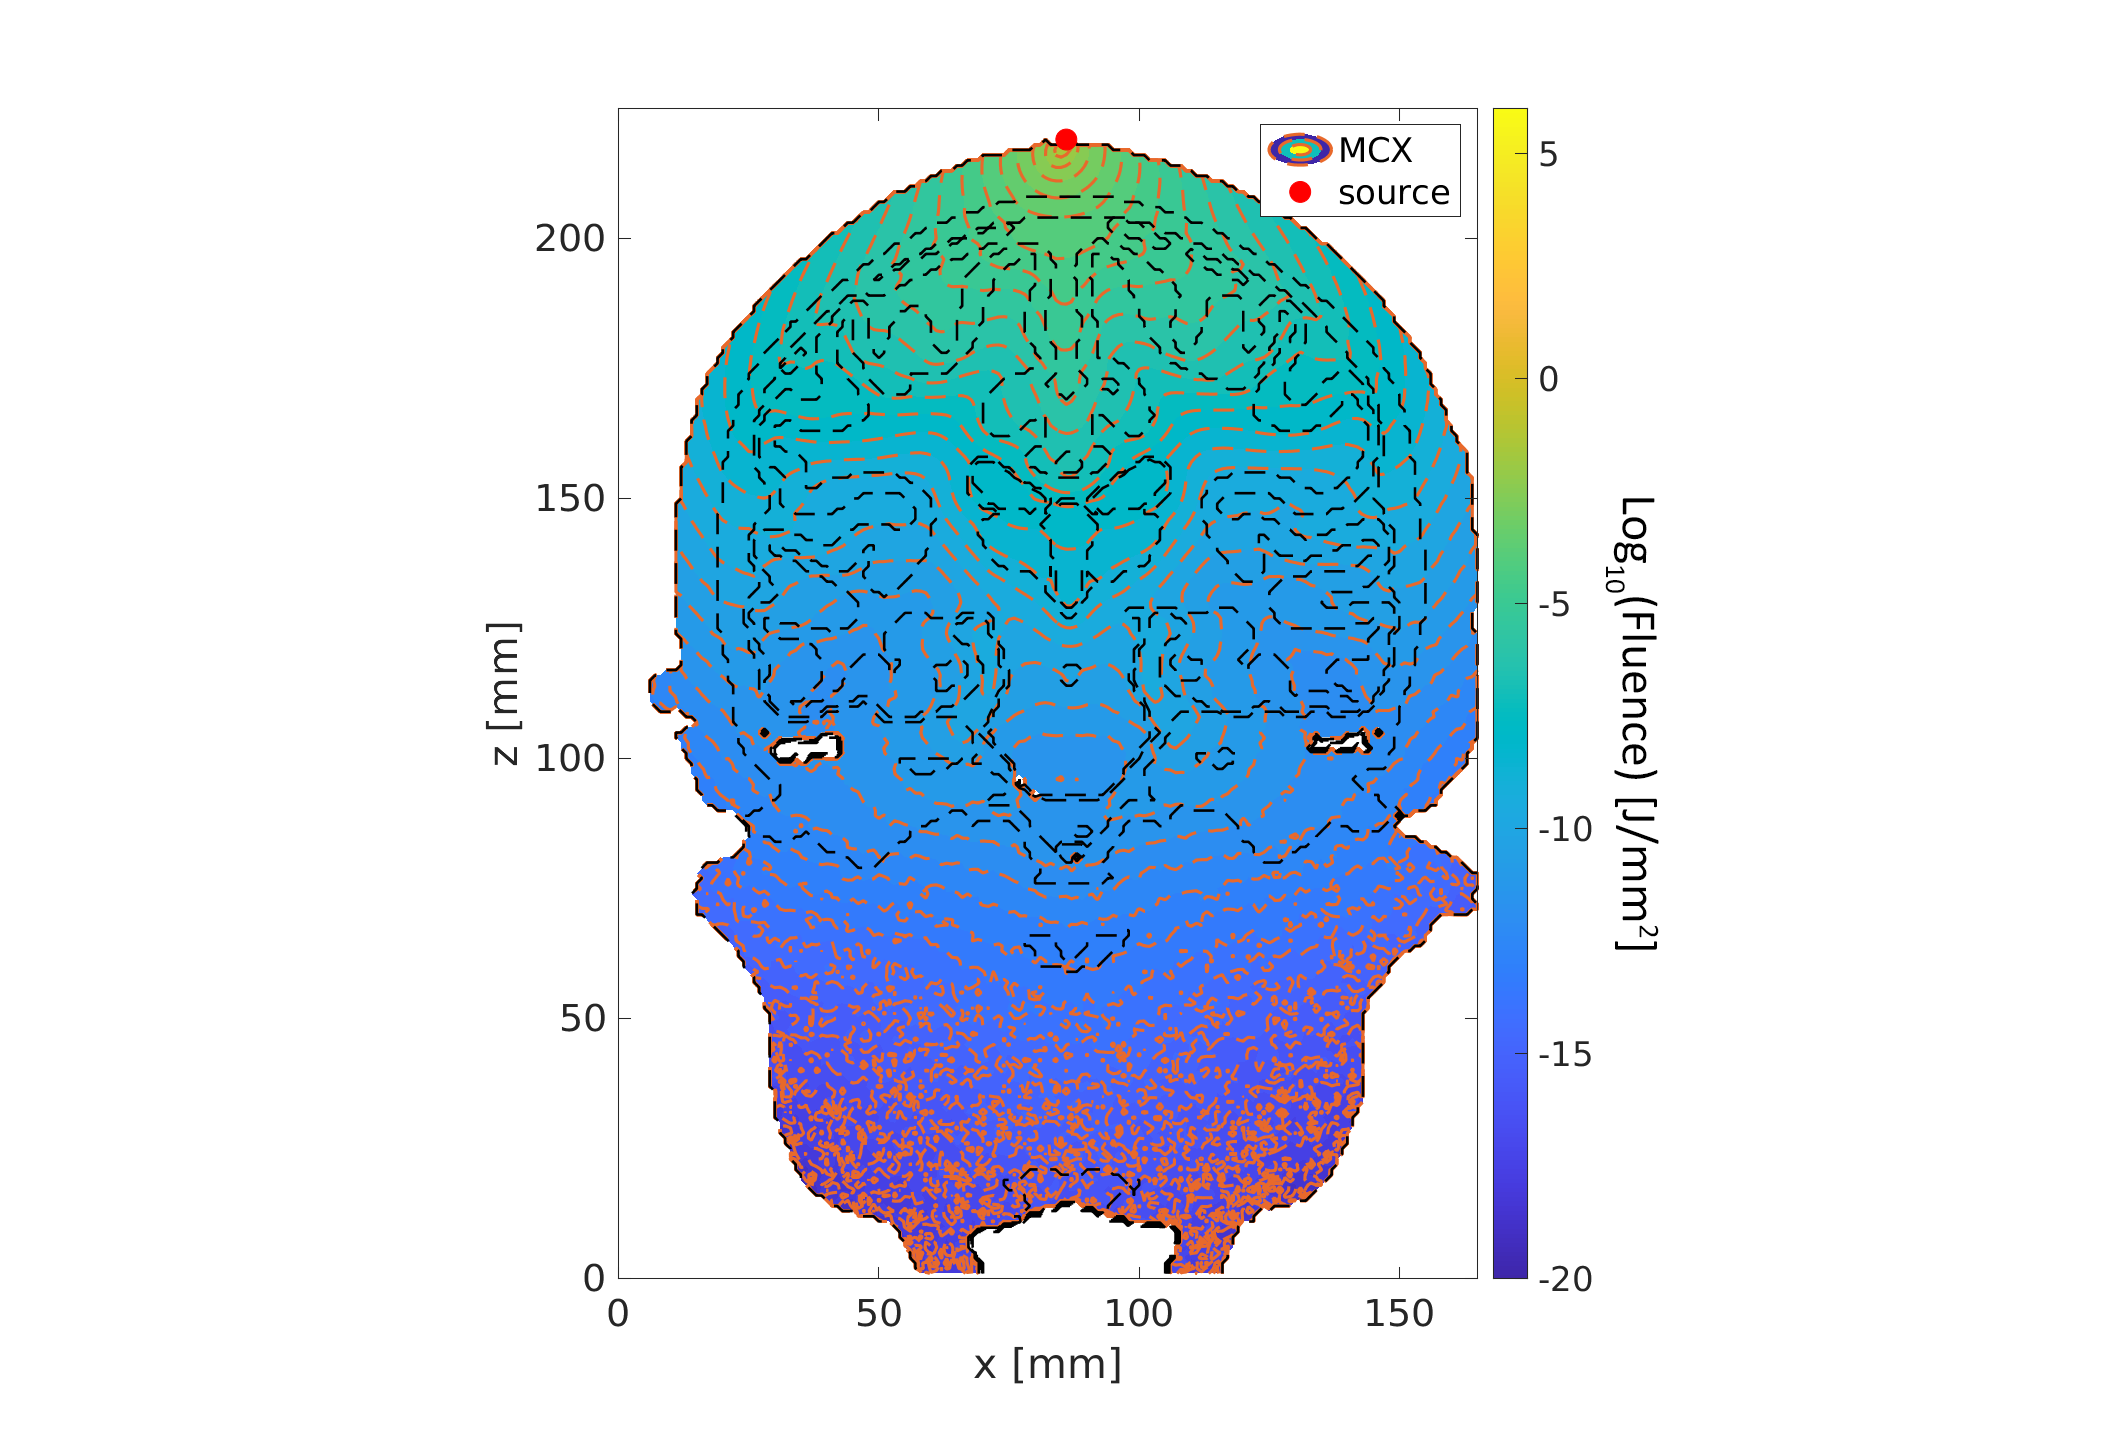
\includegraphics[width=\columnwidth]
    {Figures/Fluence_Distribution_810nm_CZ.png}}
    \caption{\label{fig:810-CZ} 810 nm CZ Position}
\end{figure}

\begin{figure}[htb!]
    \center{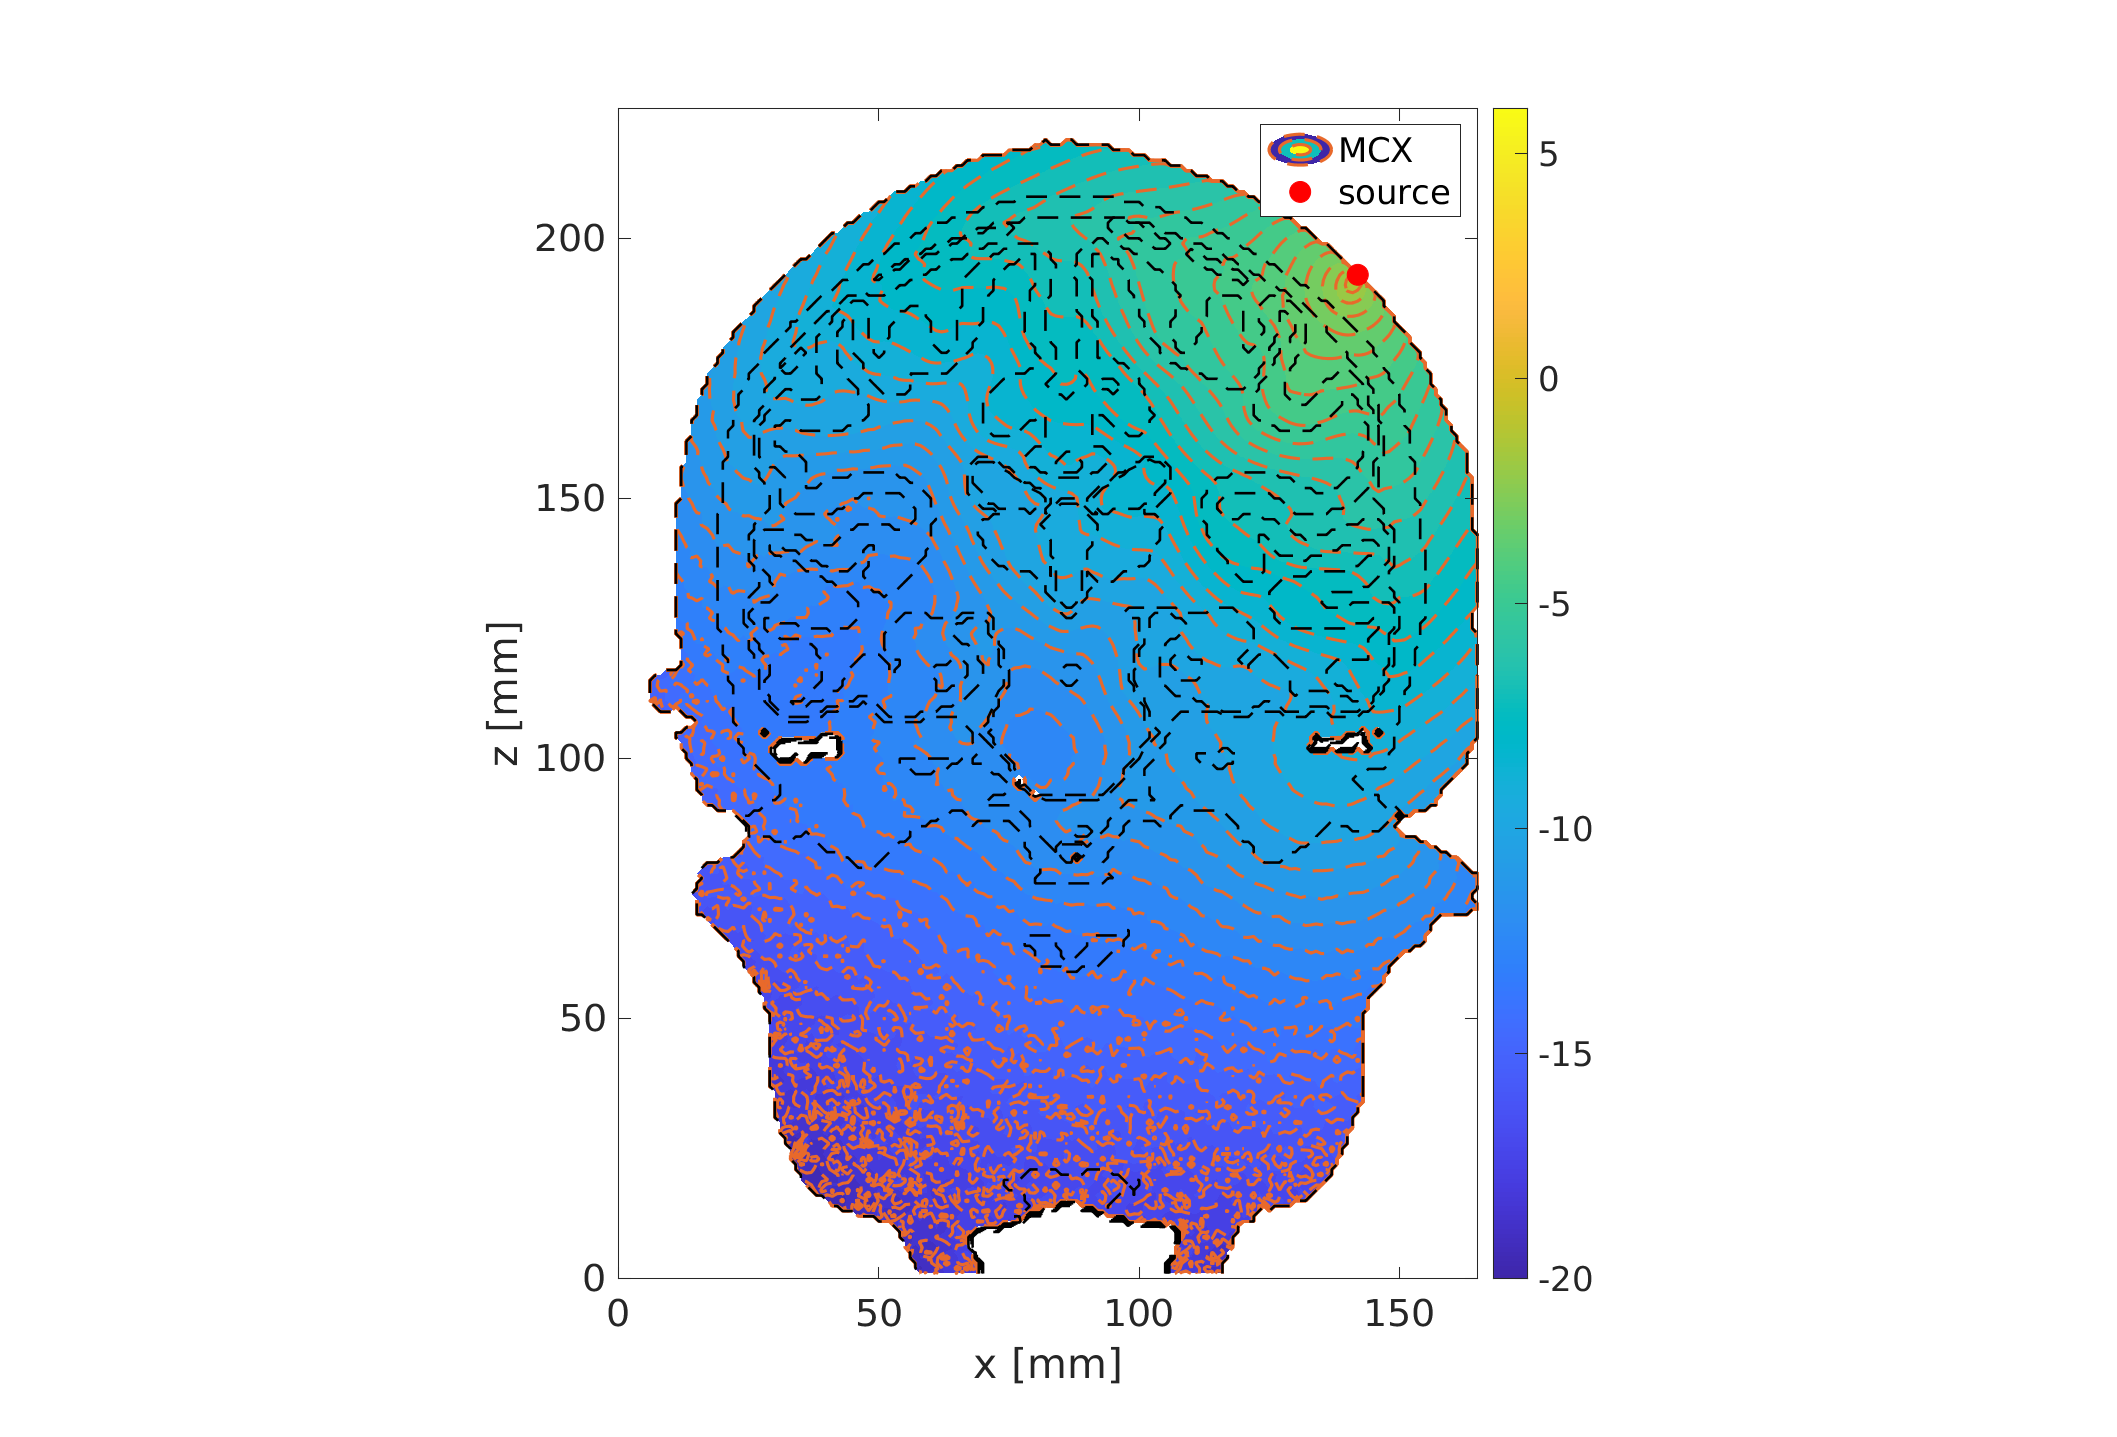
\includegraphics[width=\columnwidth]
    {Figures/Fluence_Distribution_810nm_45deg.png}}
    \caption{\label{fig:810-45} 810 nm 45 Degree Position}
\end{figure}

\begin{figure}[htb!]
    \center{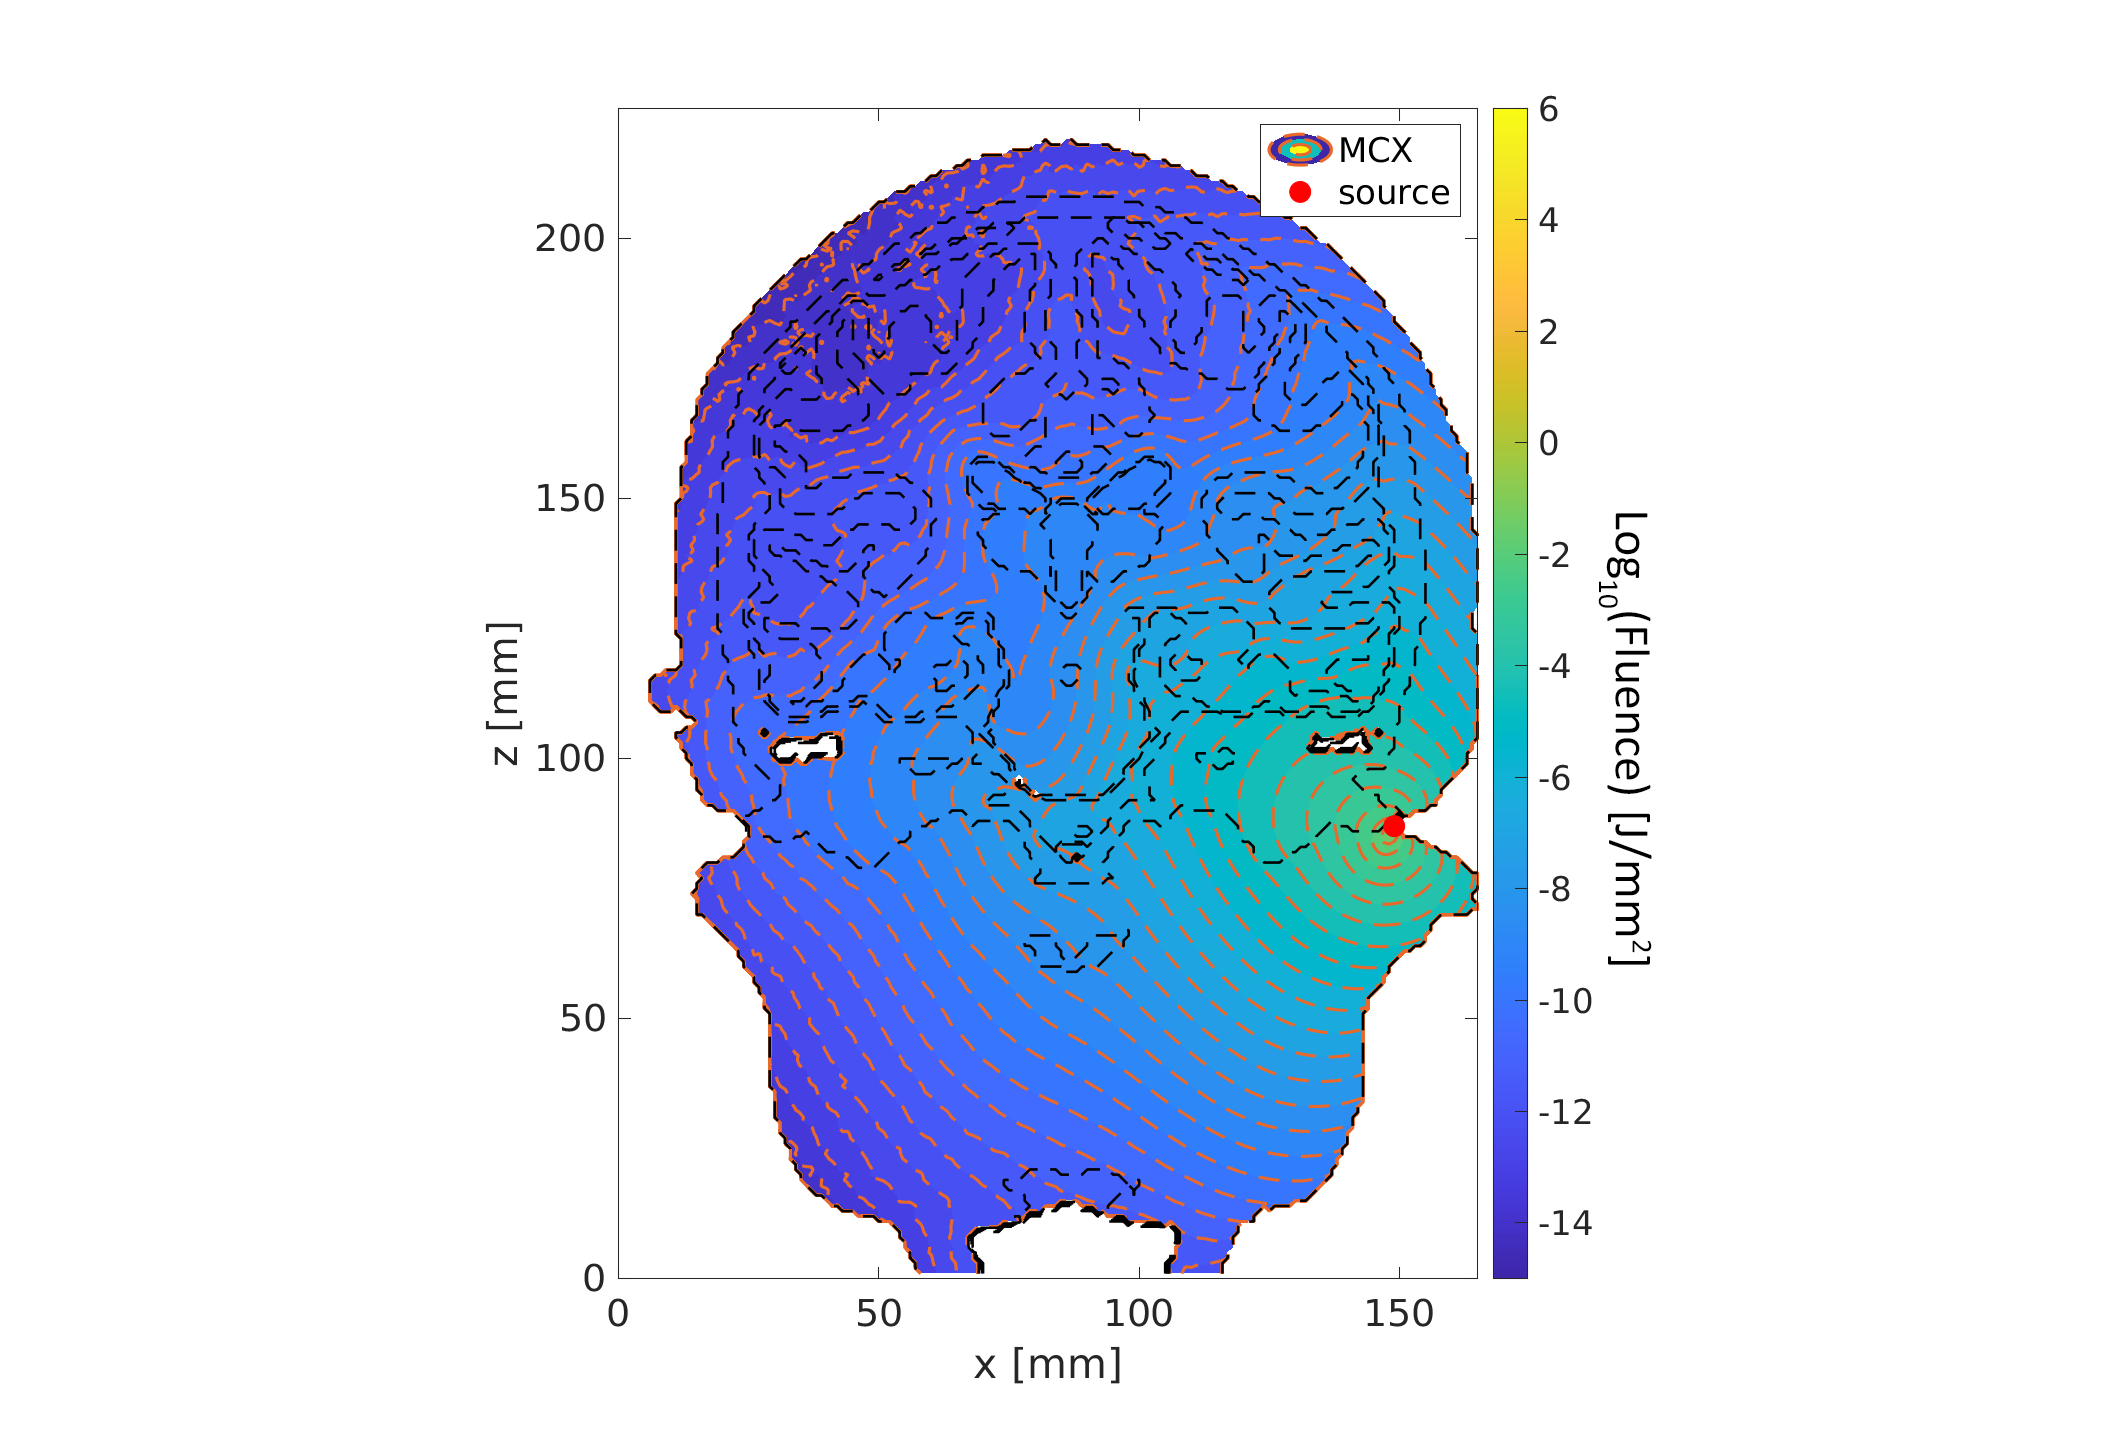
\includegraphics[width=\columnwidth]
    {Figures/Fluence_Distribution_810nm_Cochlear.png}}
    \caption{\label{fig:810-Cochlear} 810 nm Cochlear Position}
\end{figure}

\begin{figure}[htb!]
    \center{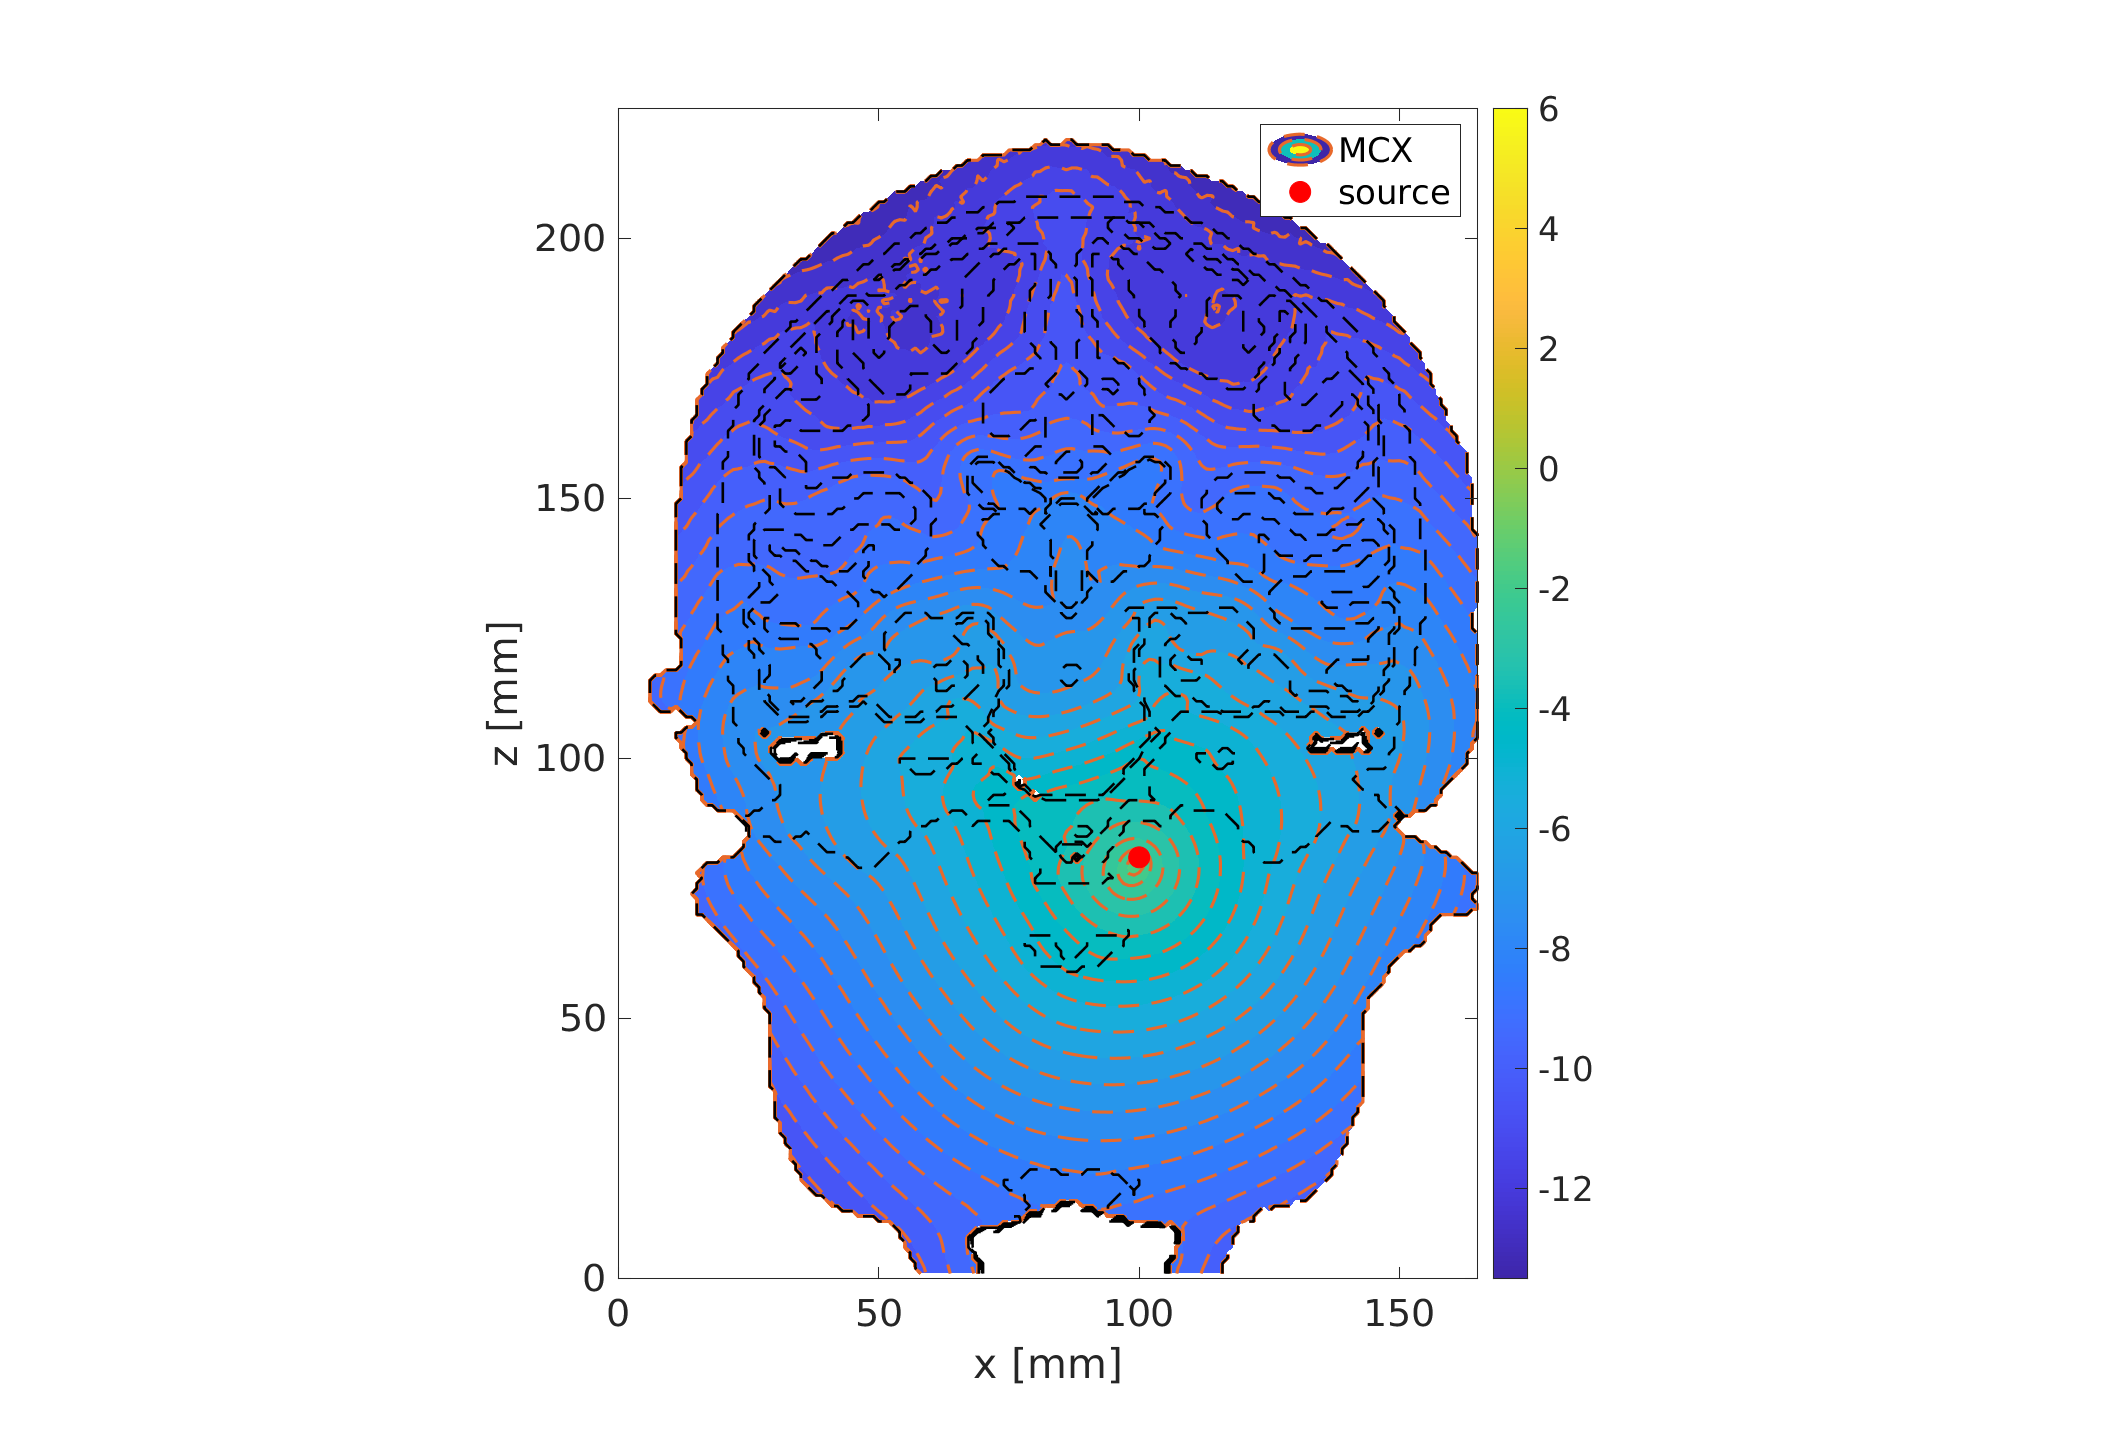
\includegraphics[width=\columnwidth]
    {Figures/Fluence_Distribution_810nm_Intranasal.png}}
    \caption{\label{fig:810-Intra} 810 nm Intranasal Position}
\end{figure}
\newpage
\section{980 nm Fluence Distribution}
\label{app:980Simulations}
\begin{figure}[htb!]
    \center{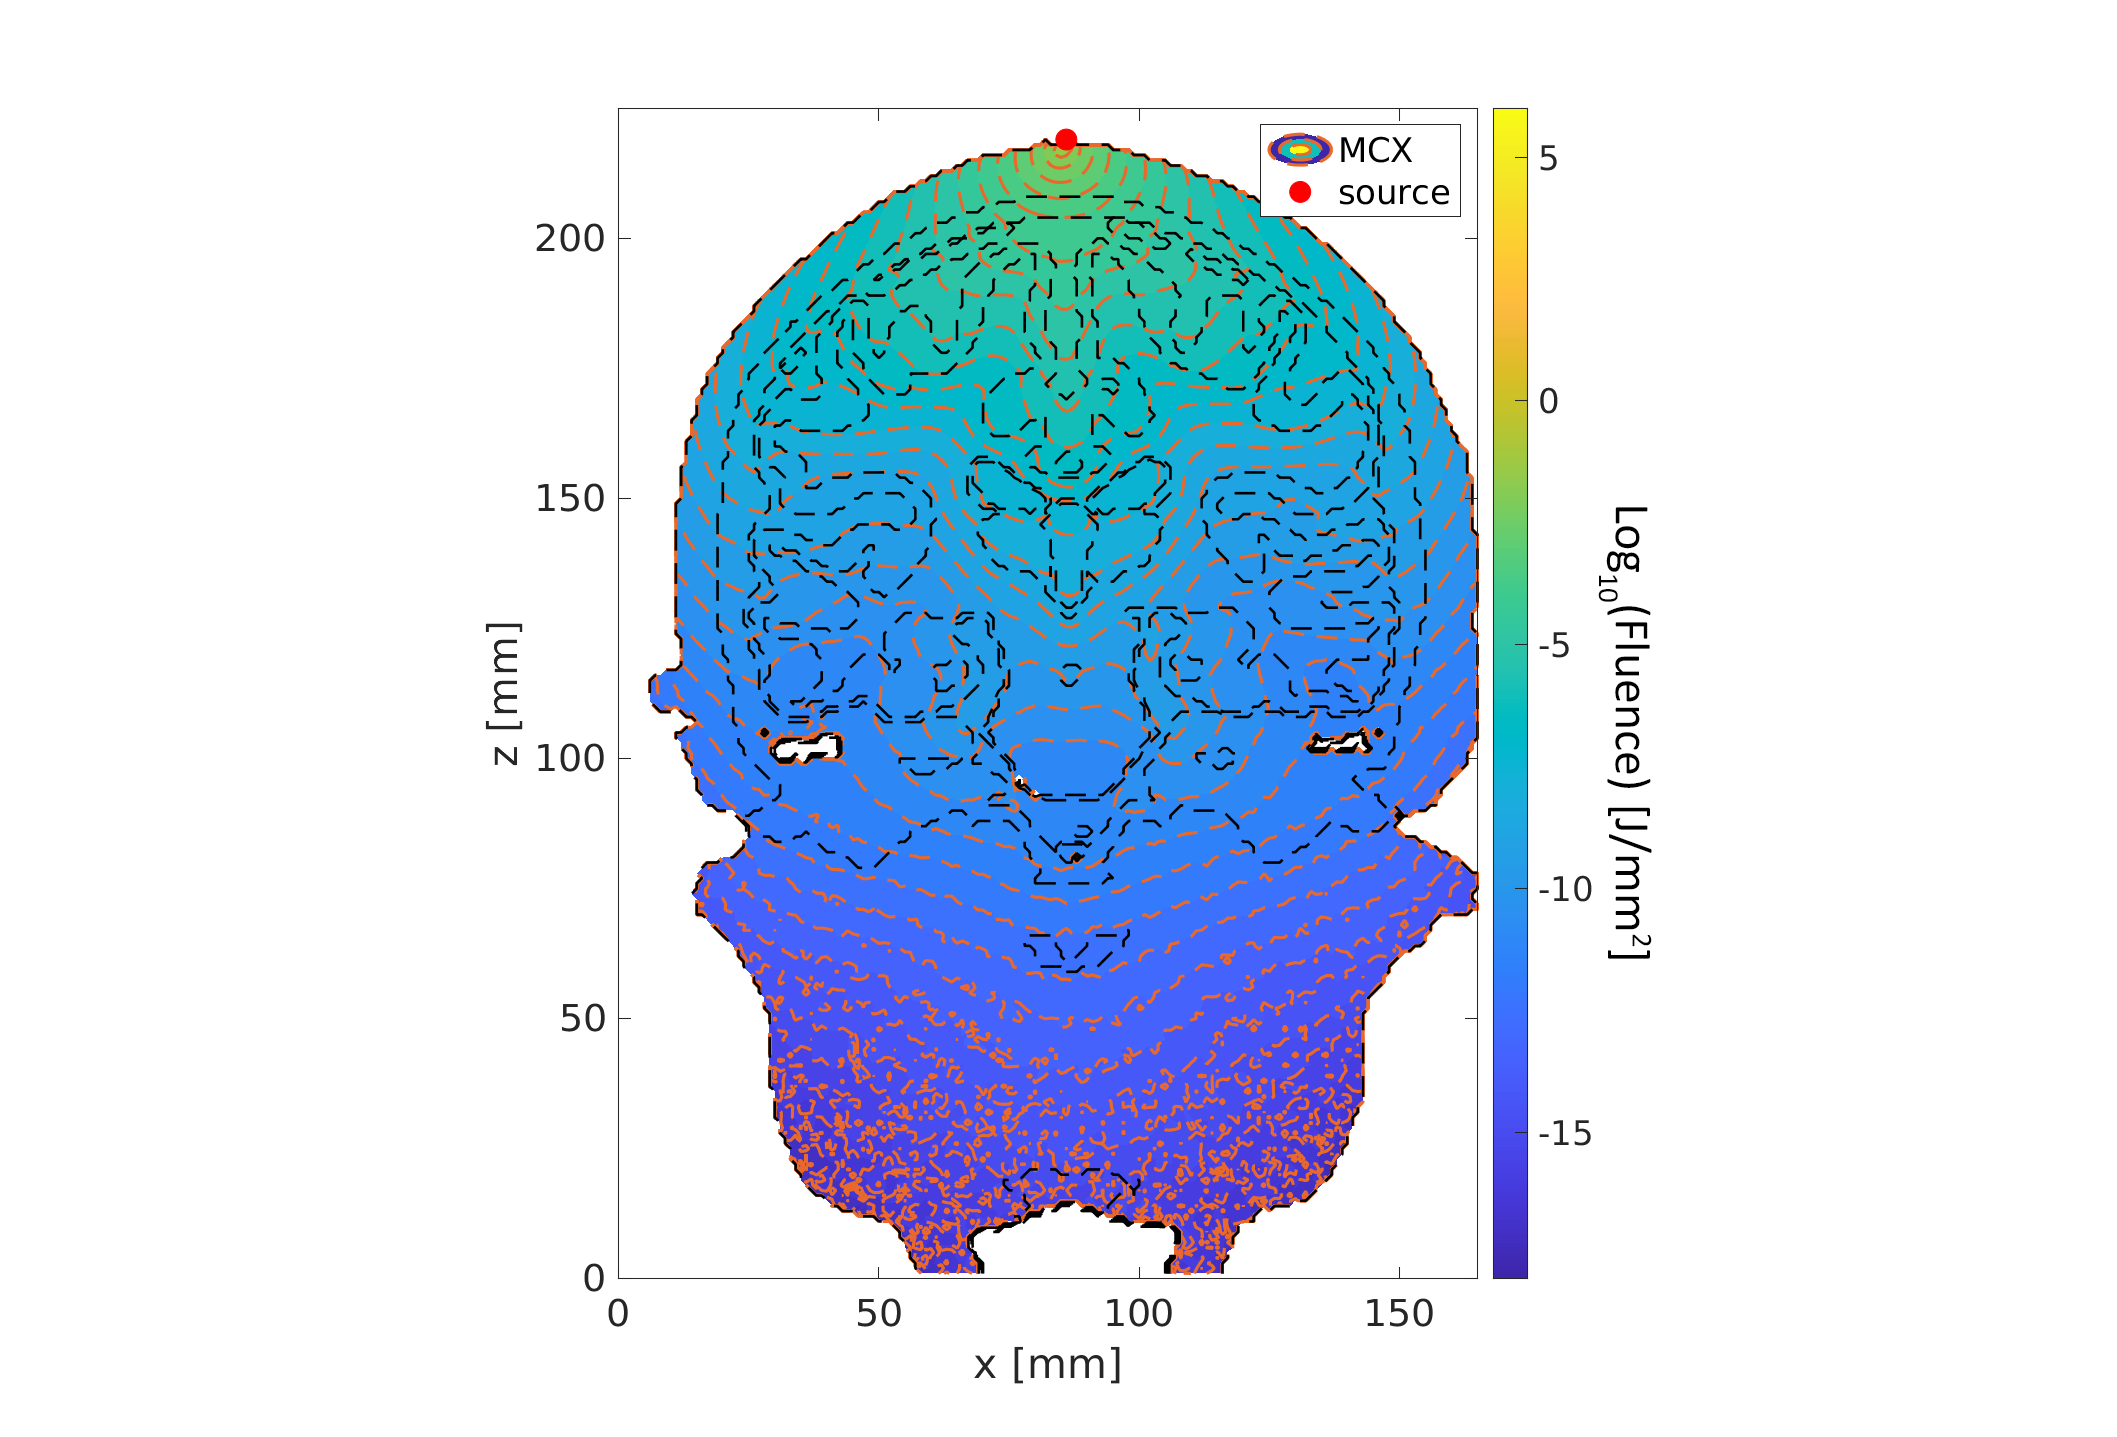
\includegraphics[width=\columnwidth]
    {Figures/Fluence_Distribution_980nm_CZ.png}}
    \caption{\label{fig:980-CZ} 980 nm CZ Position}
\end{figure}

\begin{figure}[htb!]
    \center{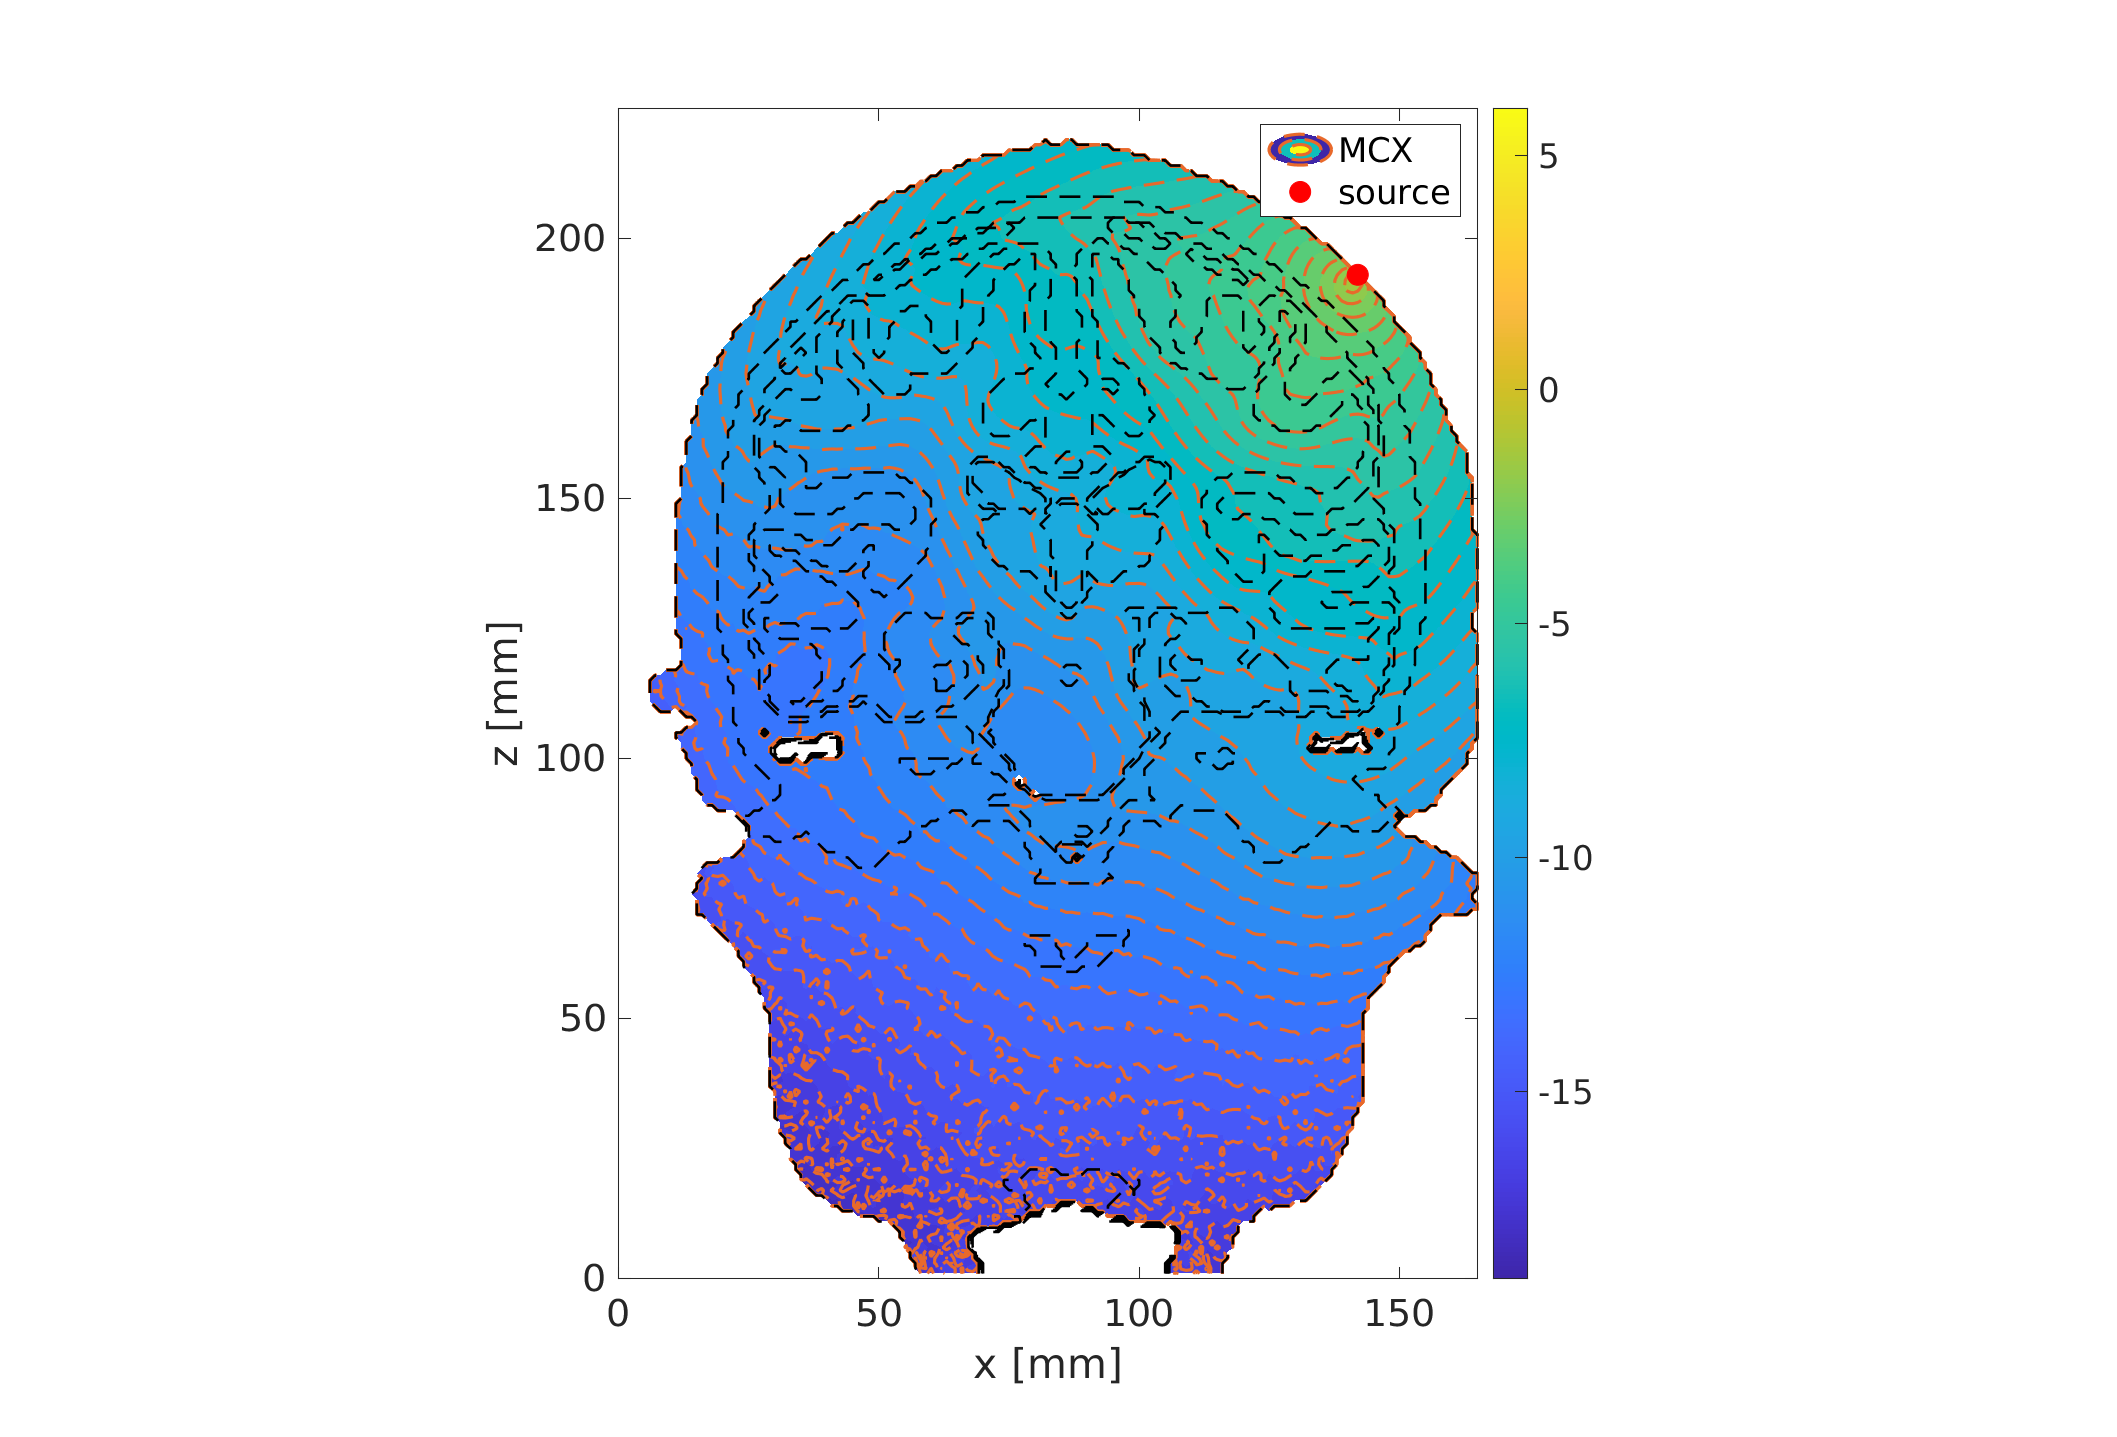
\includegraphics[width=\columnwidth]
    {Figures/Fluence_Distribution_980nm_45deg.png}}
    \caption{\label{fig:980-45} 980 nm 45 Degree Position}
\end{figure}

\begin{figure}[htb!]
    \center{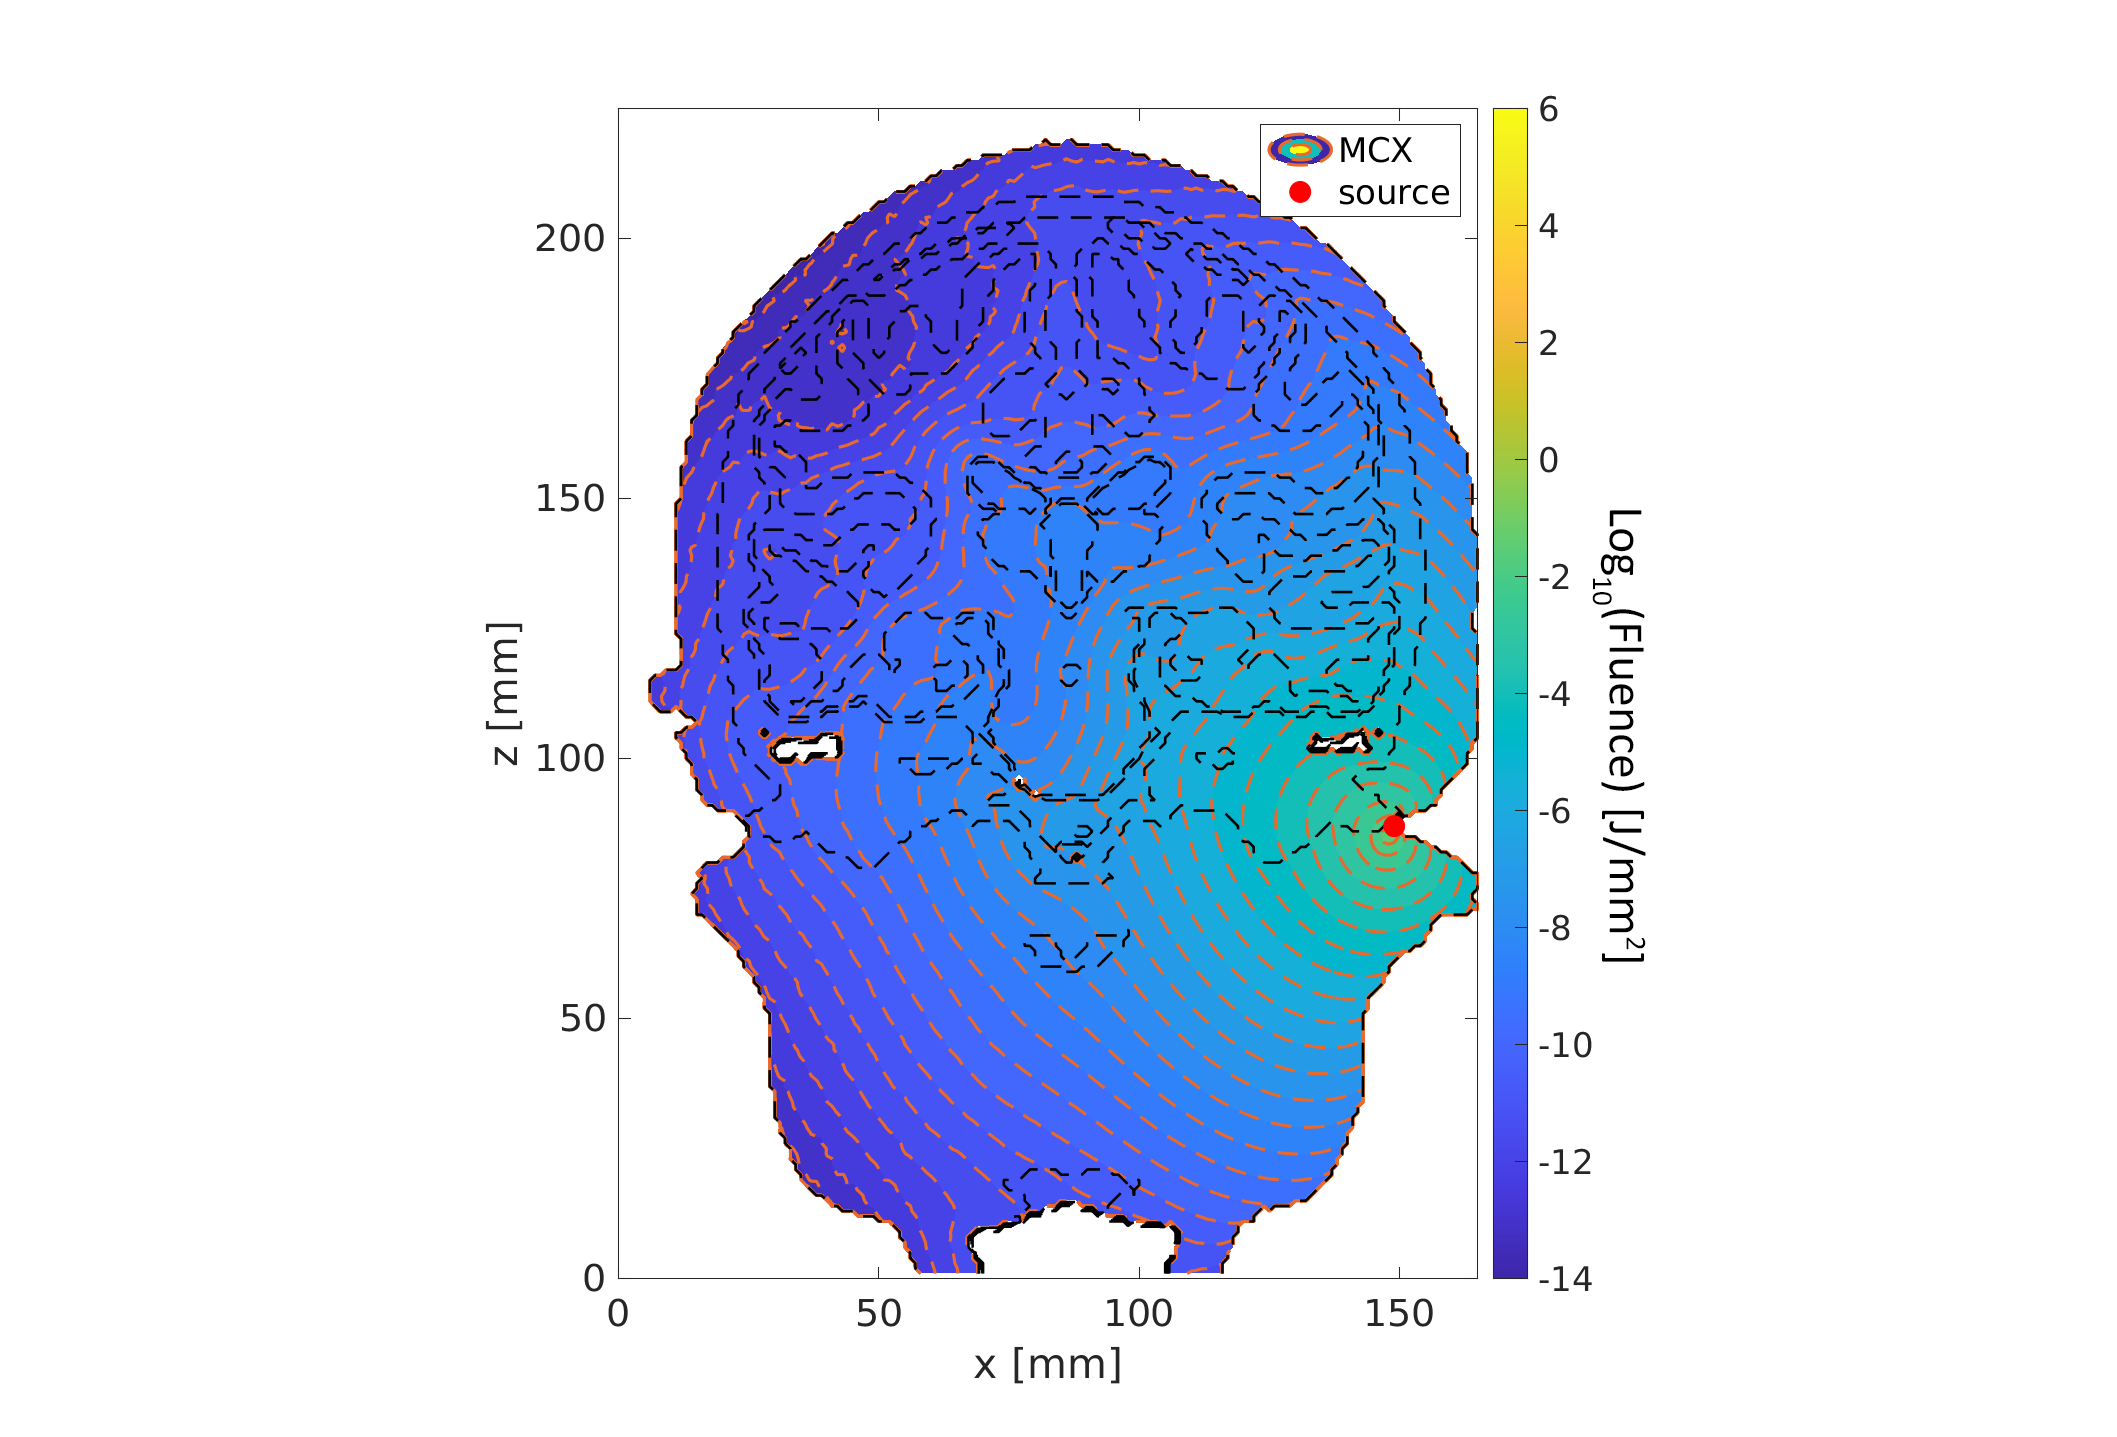
\includegraphics[width=\columnwidth]
    {Figures/Fluence_Distribution_980nm_Cochlear.png}}
    \caption{\label{fig:980-Cochlear} 980 nm Cochlear Position}
\end{figure}

\begin{figure}[htb!]
    \center{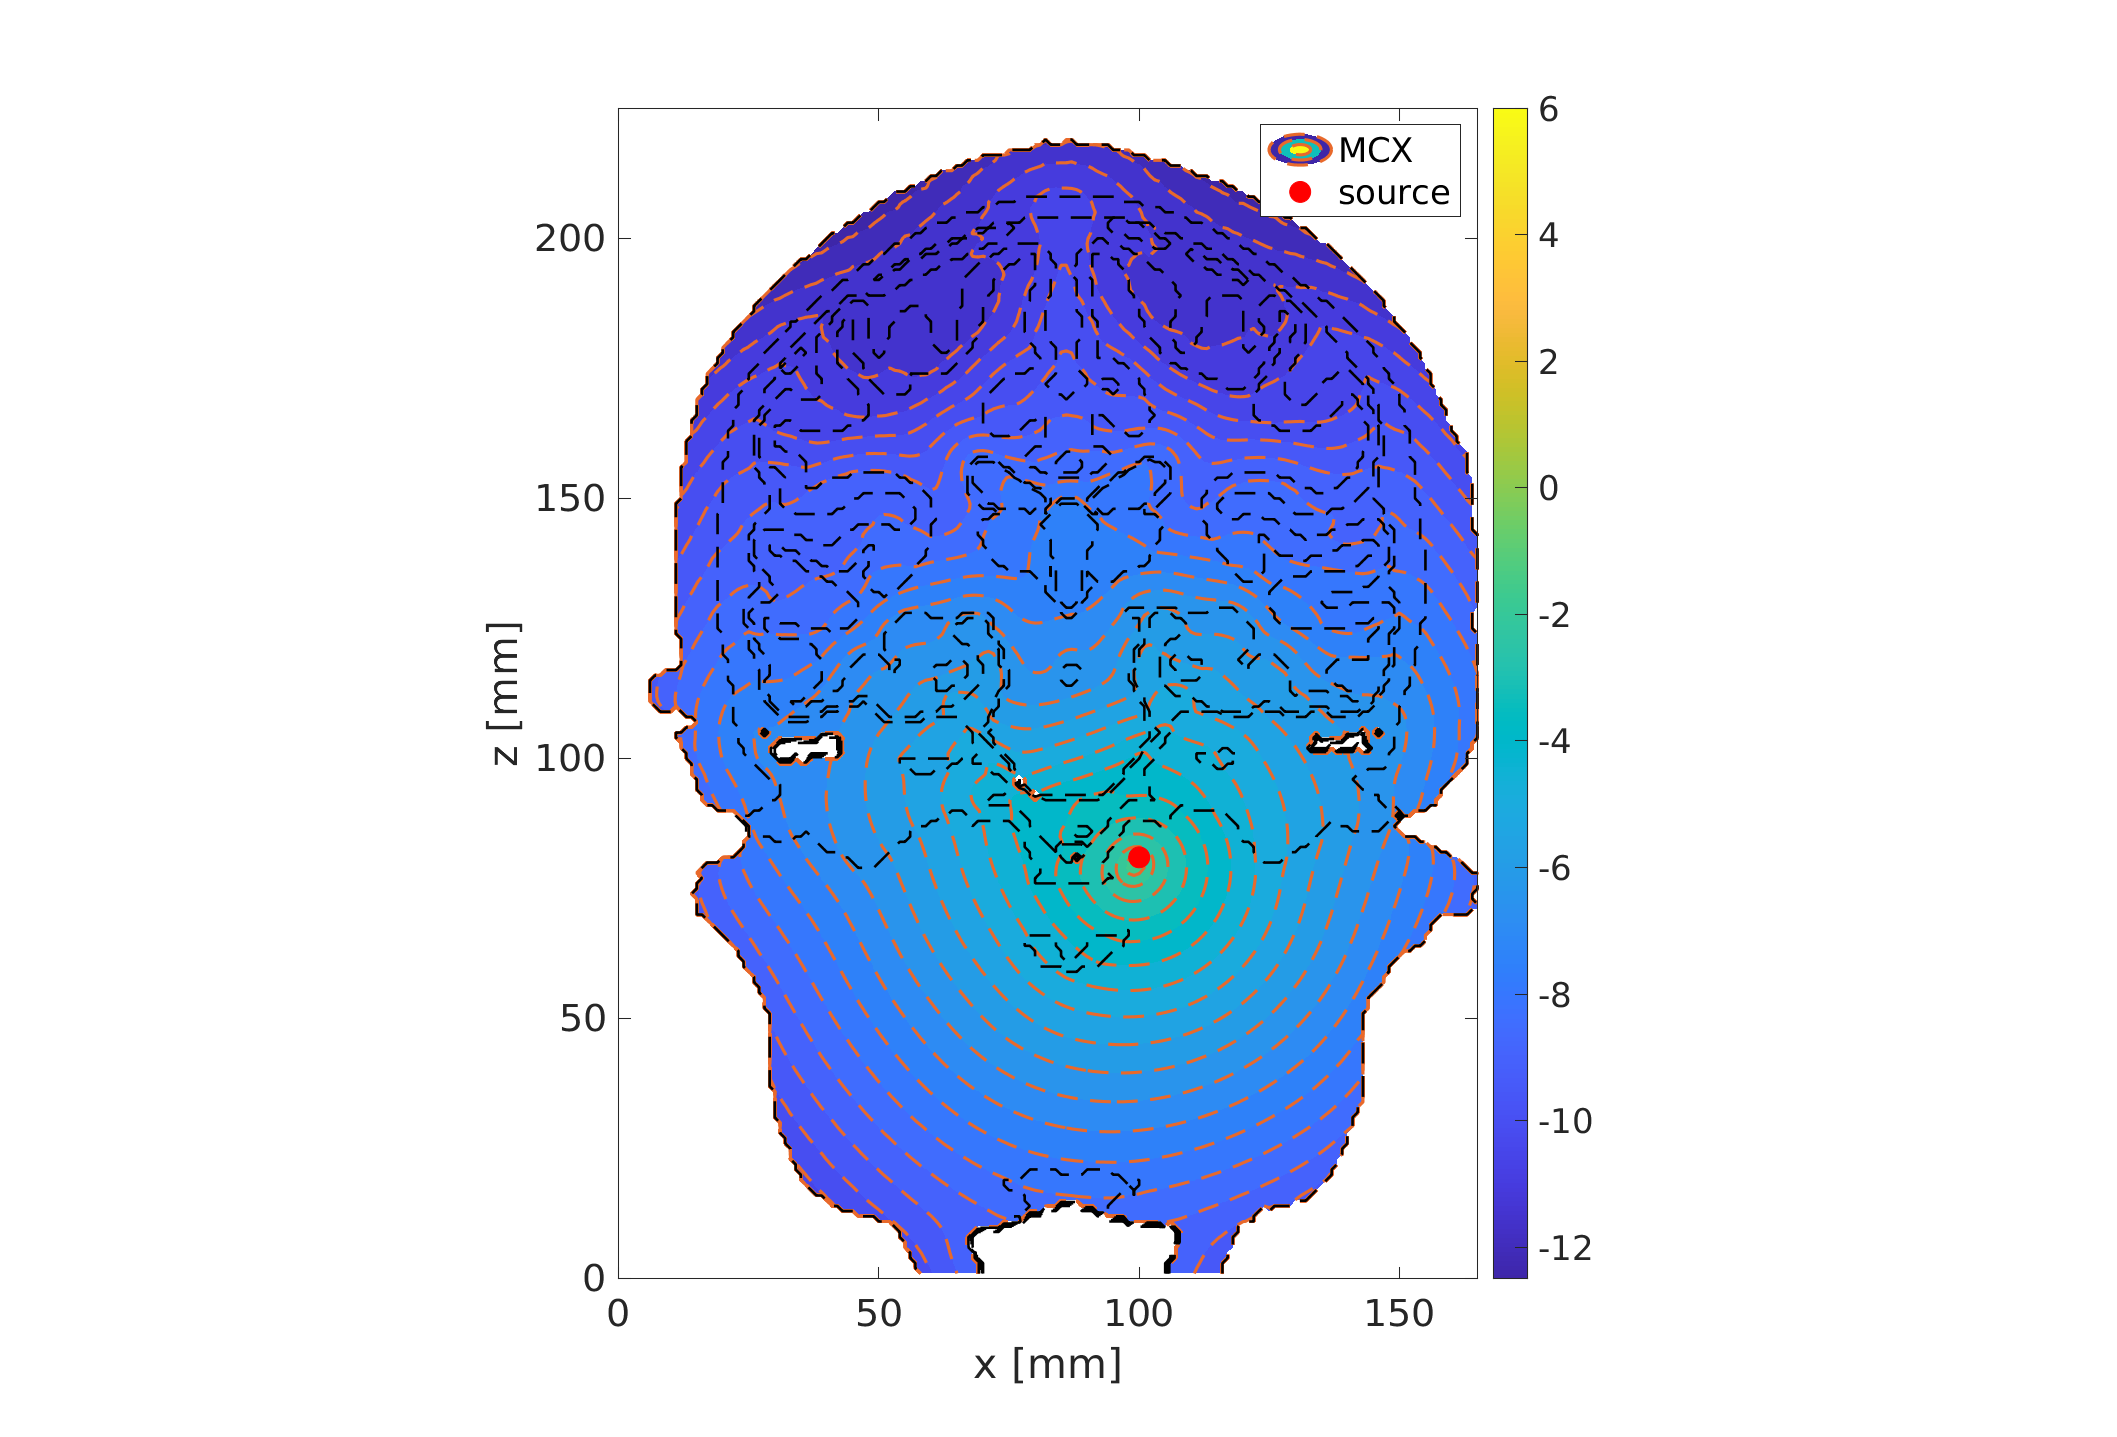
\includegraphics[width=\columnwidth]
    {Figures/Fluence_Distribution_980nm_Intranasal.png}}
    \caption{\label{fig:980-Intra} 980 nm Intranasal Position}
\end{figure}
\newpage
\section{1064 nm Fluence Distribution}
\label{app:1064Simulations}
\begin{figure}[htb!]
    \center{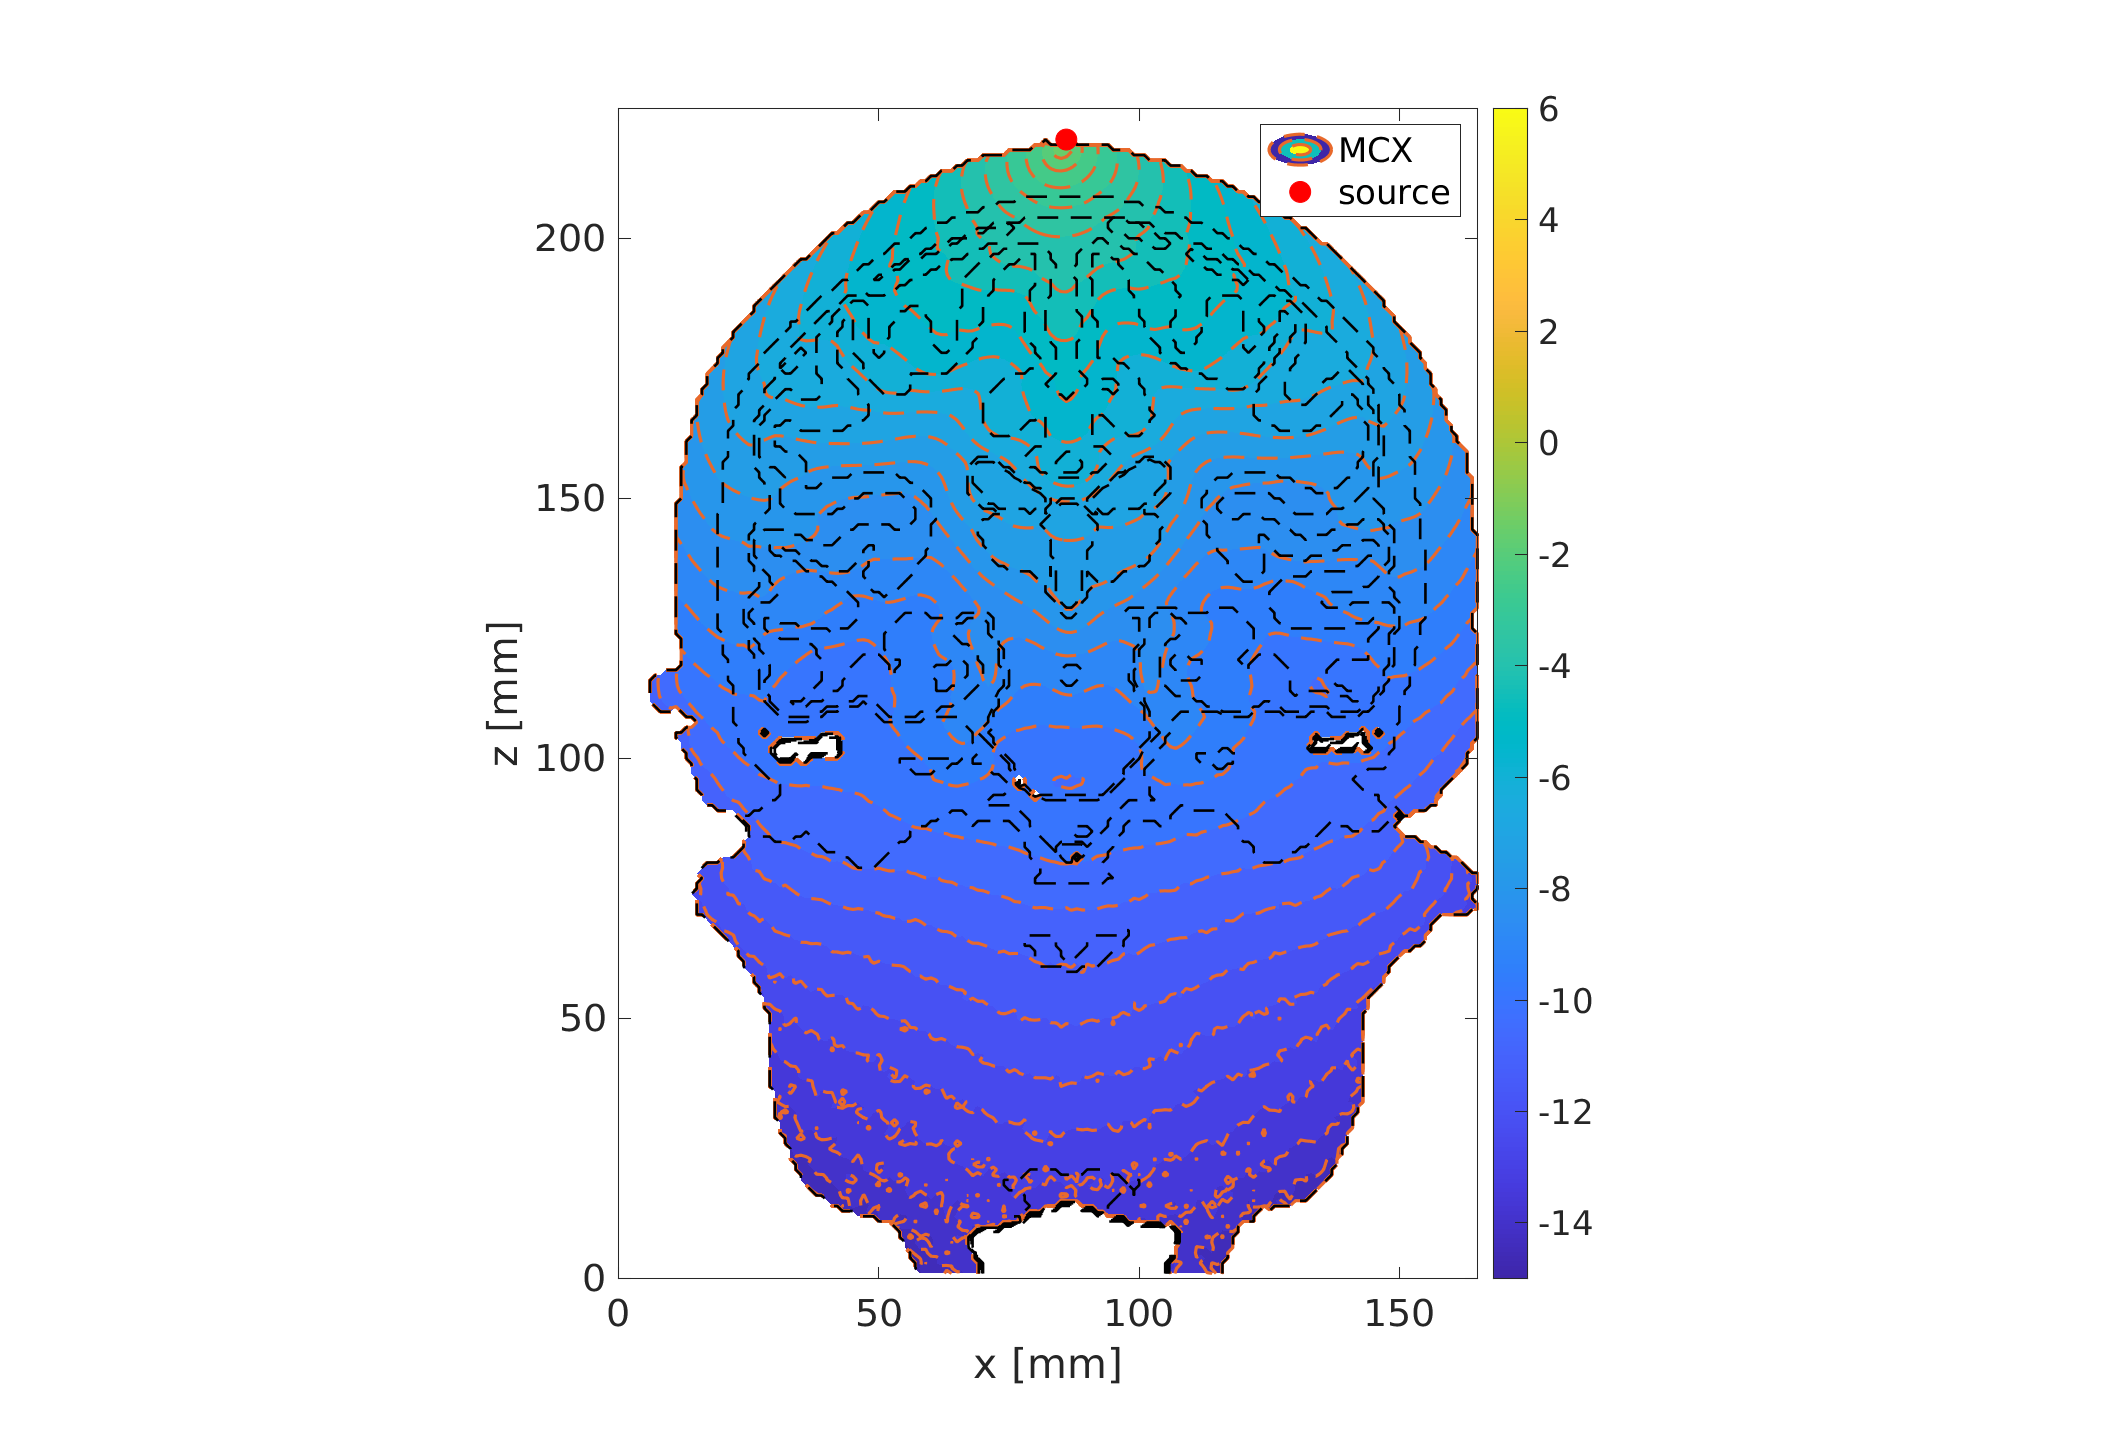
\includegraphics[width=\columnwidth]
    {Figures/Fluence_Distribution_1064nm_CZ.png}}
    \caption{\label{fig:1064-CZ} 1064 nm CZ Position}
\end{figure}

\begin{figure}[htb!]
    \center{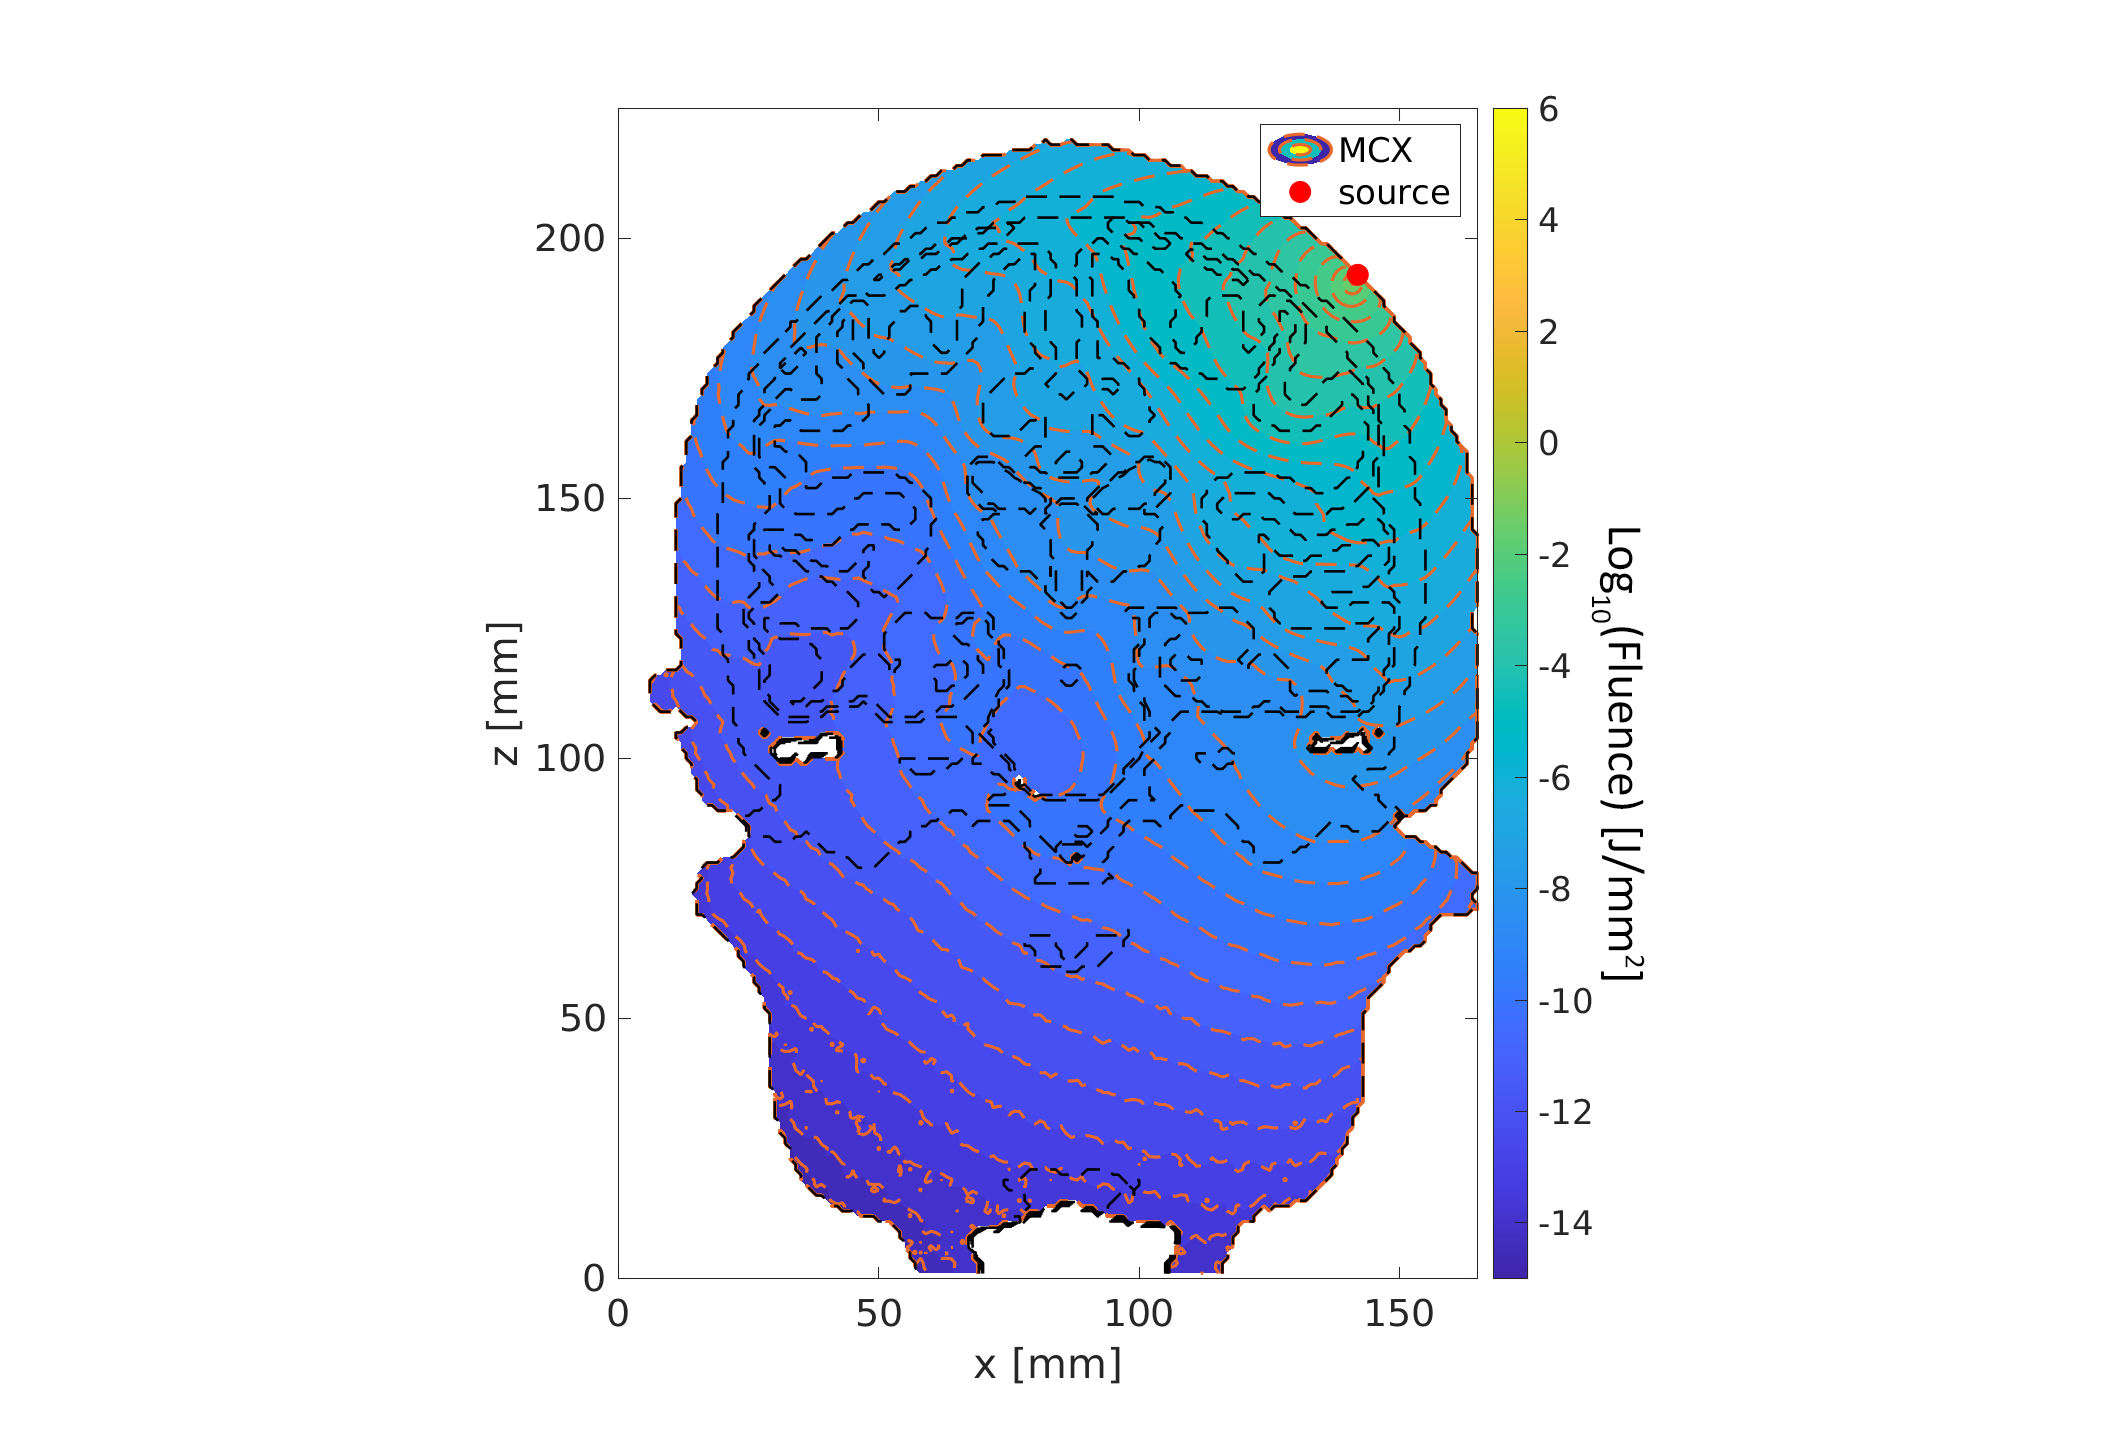
\includegraphics[width=\columnwidth]
    {Figures/Fluence_Distribution_1064nm_45deg.png}}
    \caption{\label{fig:1064-45} 1064 nm 45 Degree Position}
\end{figure}

\begin{figure}[htb!]
    \center{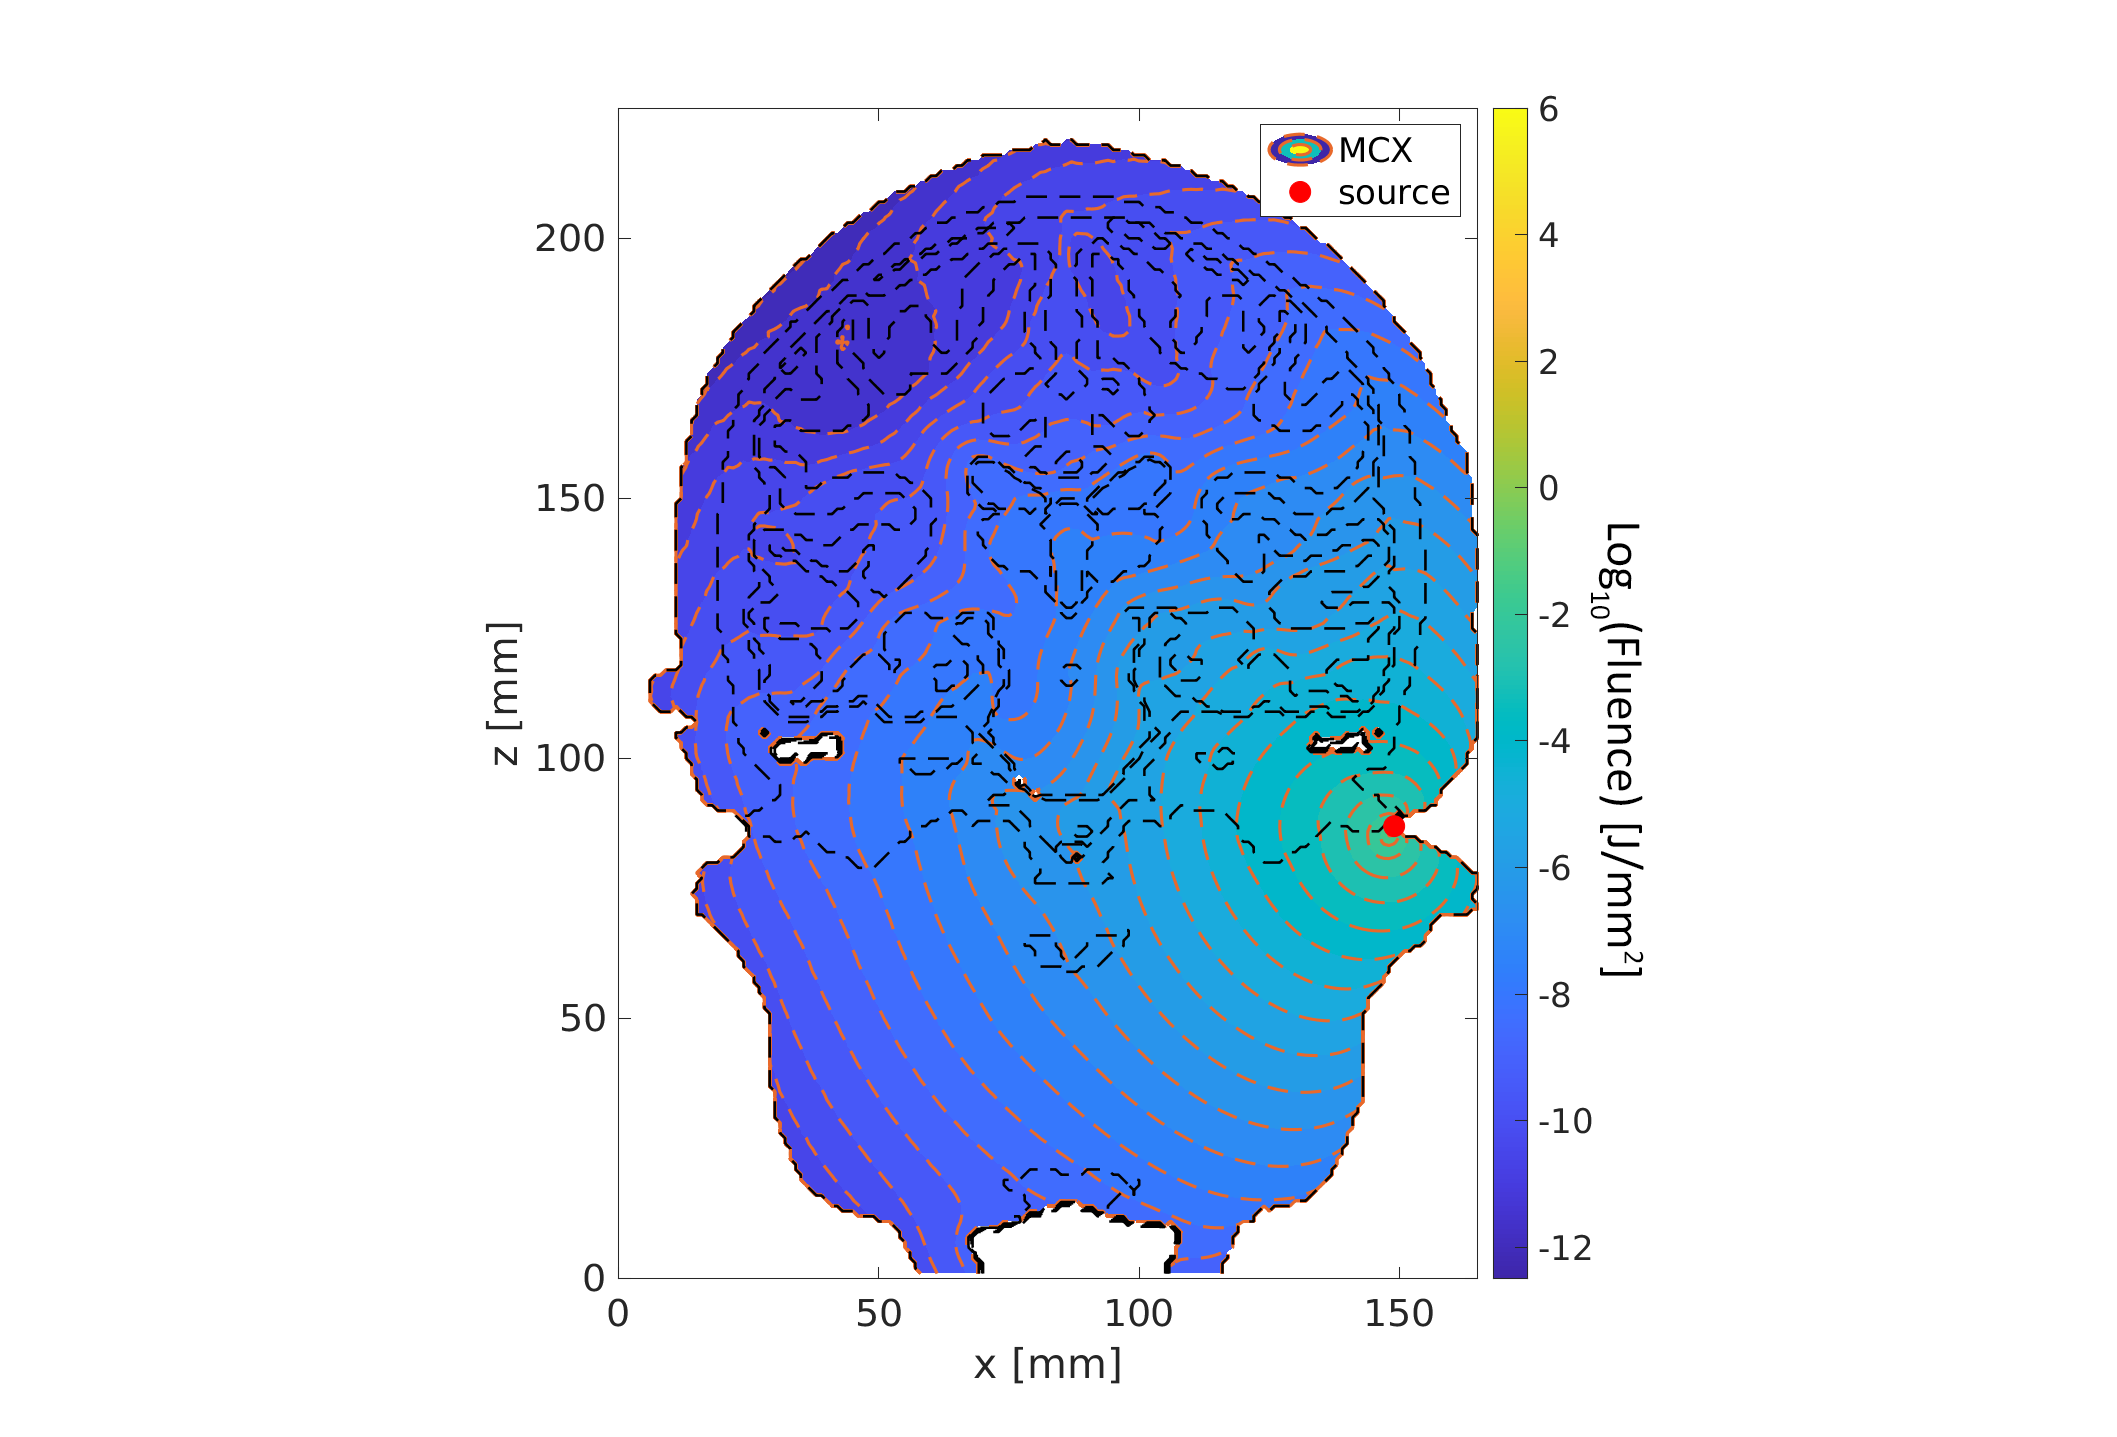
\includegraphics[width=\columnwidth]
    {Figures/Fluence_Distribution_1064nm_Cochlear.png}}
    \caption{\label{fig:1064-Cochlear} 1064 nm Cochlear Position}
\end{figure}

\begin{figure}[htb!]
    \center{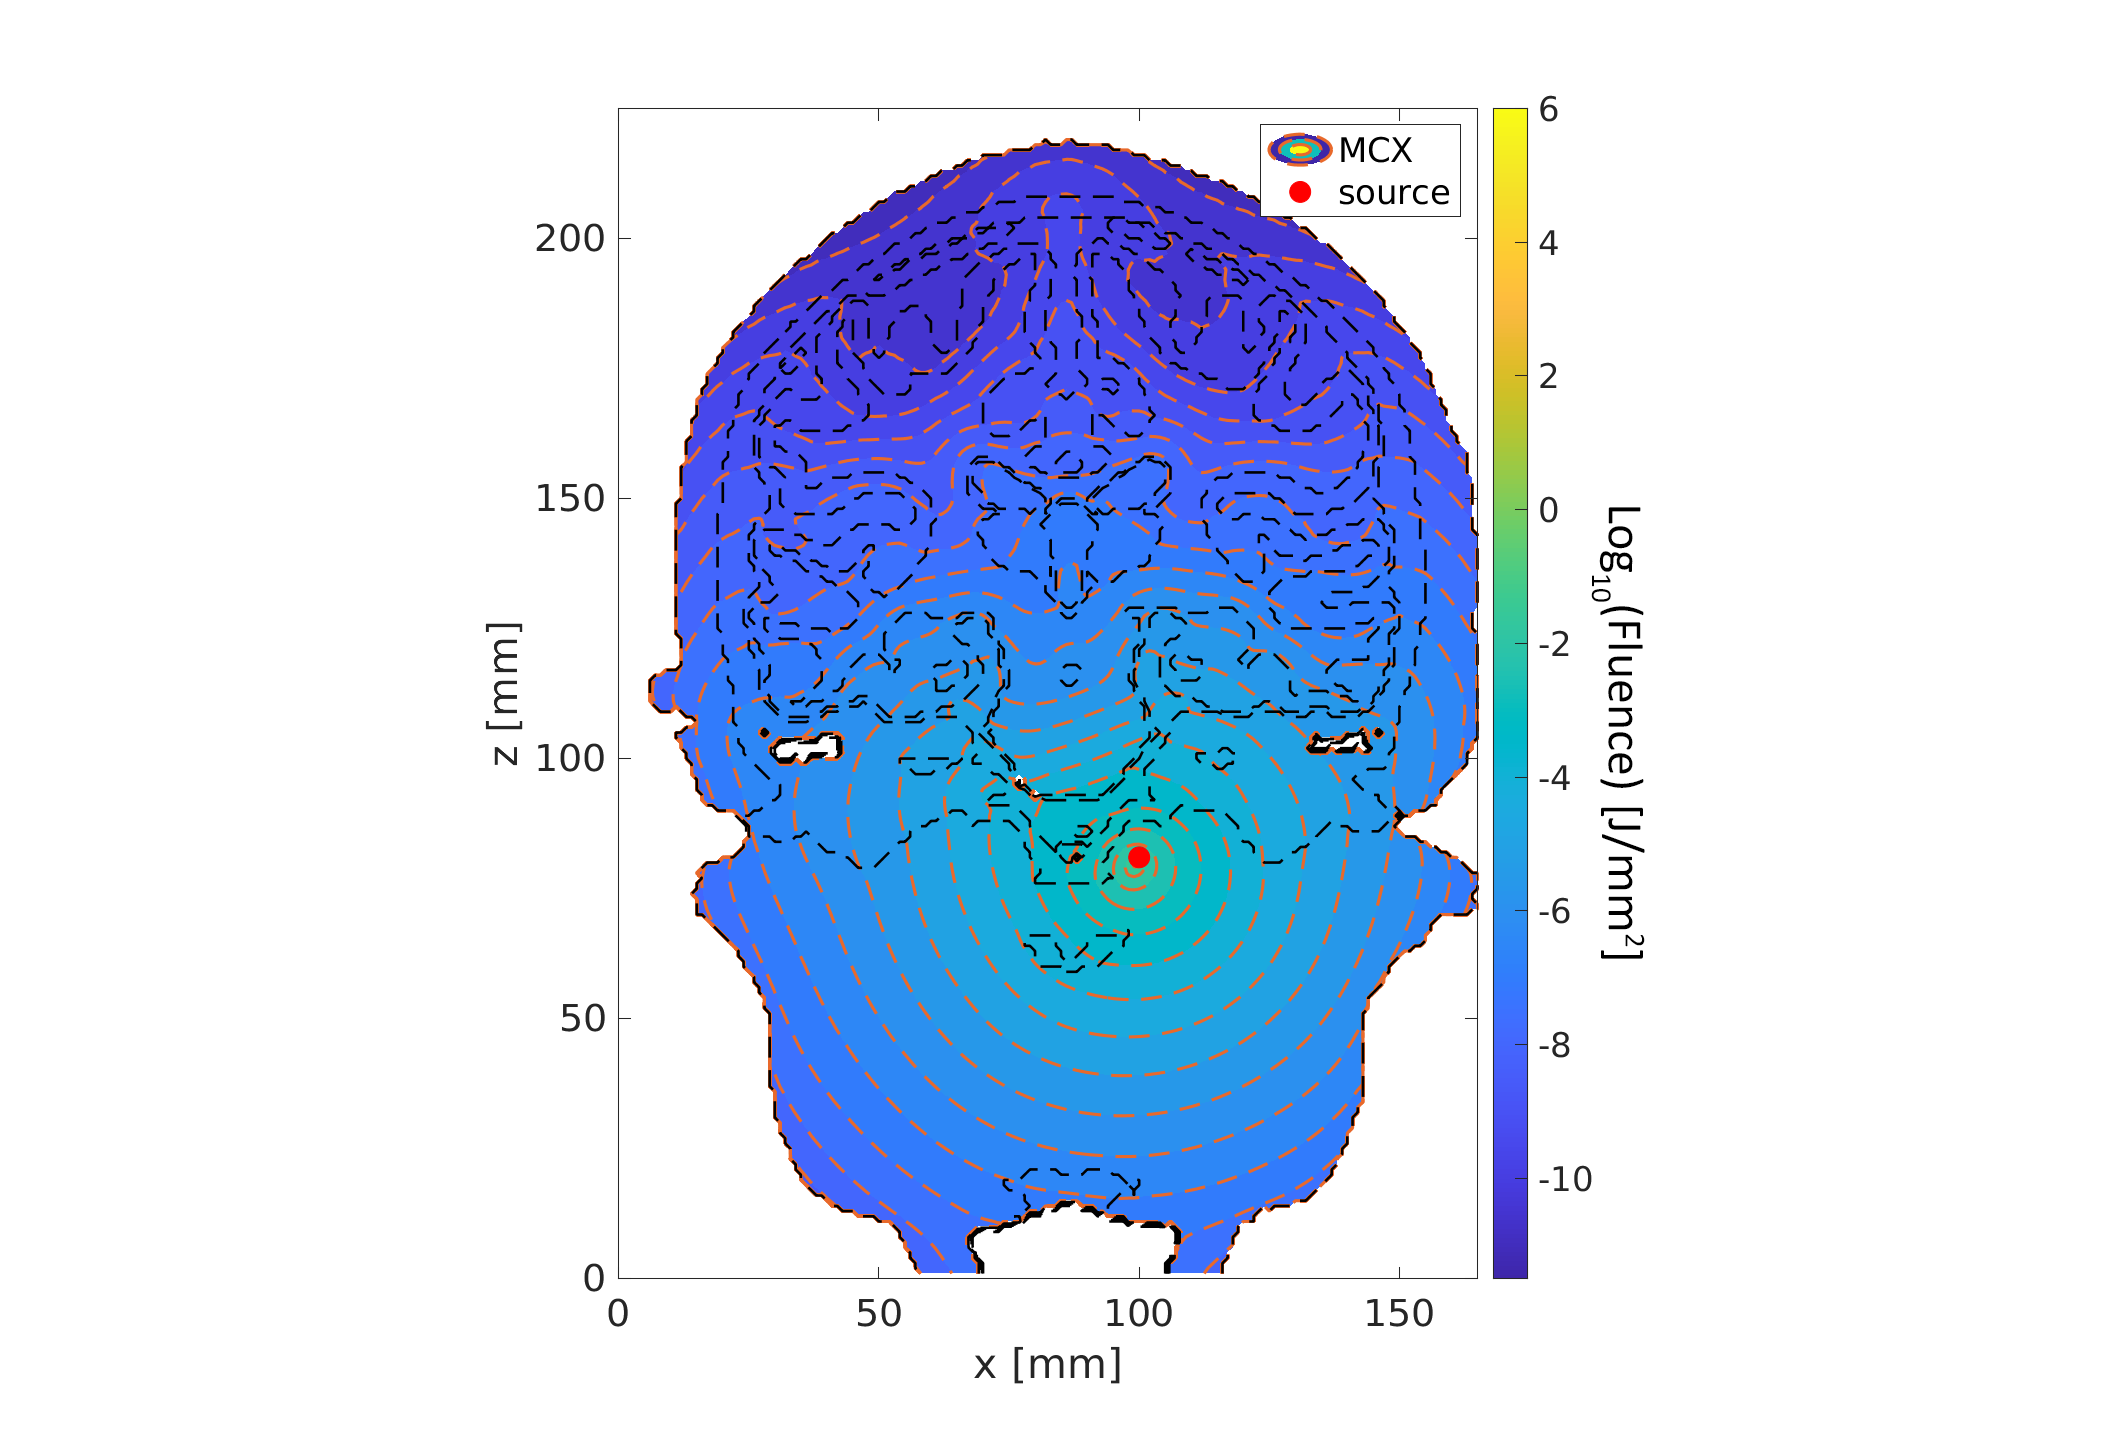
\includegraphics[width=\columnwidth]
    {Figures/Fluence_Distribution_1064nm_Intranasal.png}}
    \caption{\label{fig:1064-Intra} 1064 nm Intranasal Position}
\end{figure}
\newpage
\section{1550 nm Fluence Distribution}
\label{app:1550Simulations}
\begin{figure}[htb!]
    \center{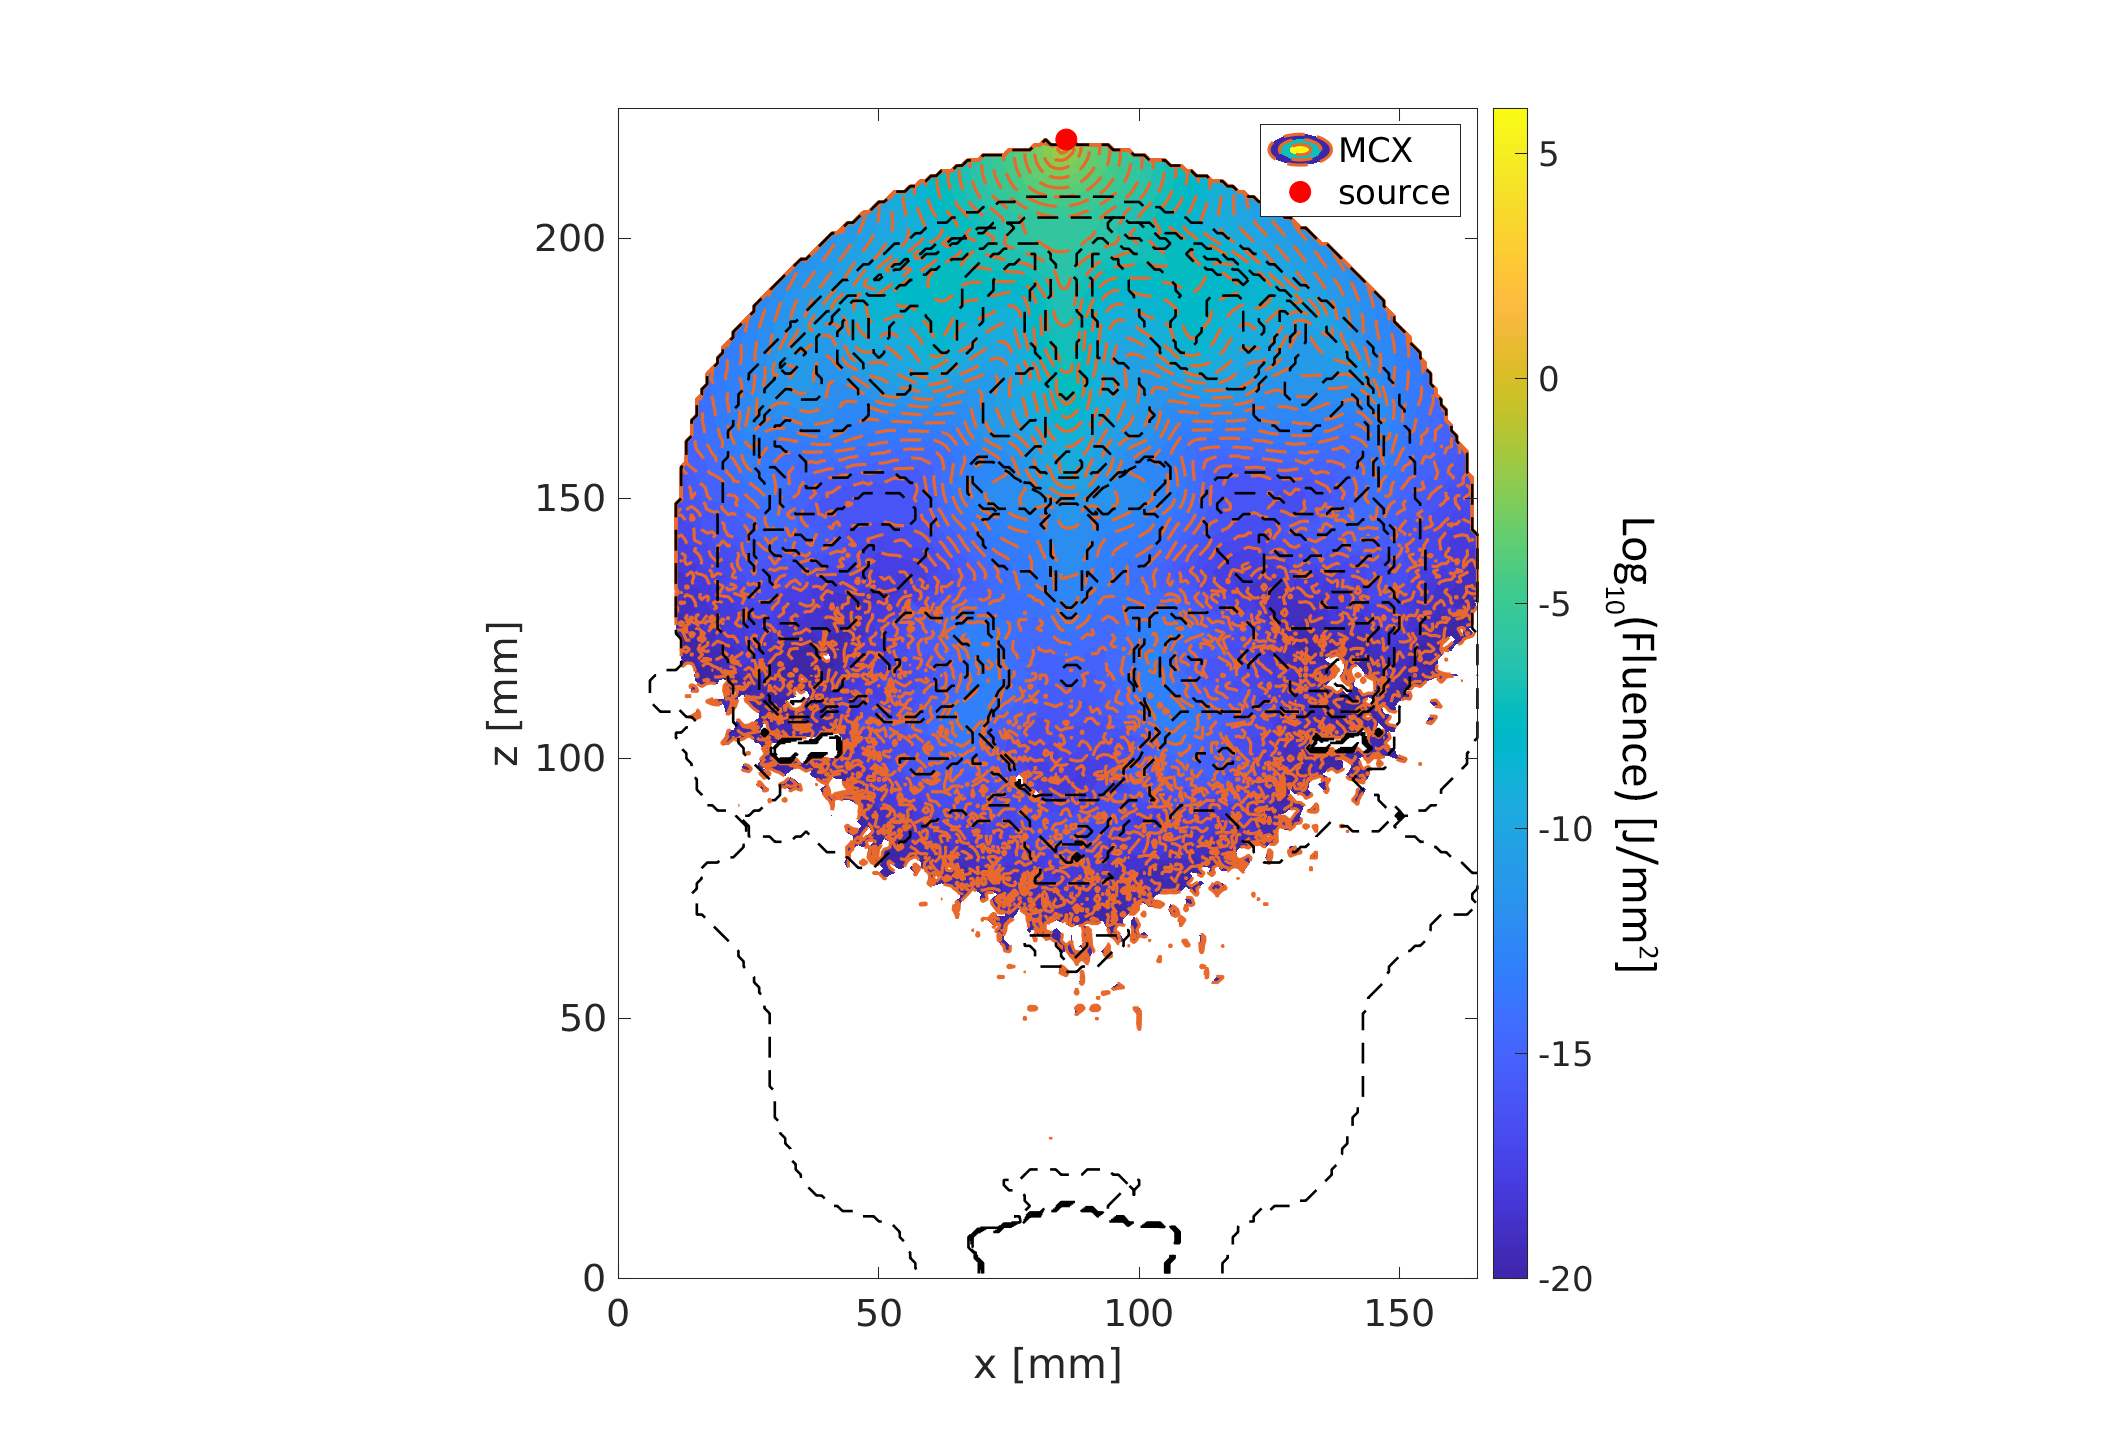
\includegraphics[width=\columnwidth]
    {Figures/Fluence_Distribution_1550nm_CZ.png}}
    \caption{\label{fig:1550-CZ} 1550 nm CZ Position}
\end{figure}

\begin{figure}[htb!]
    \center{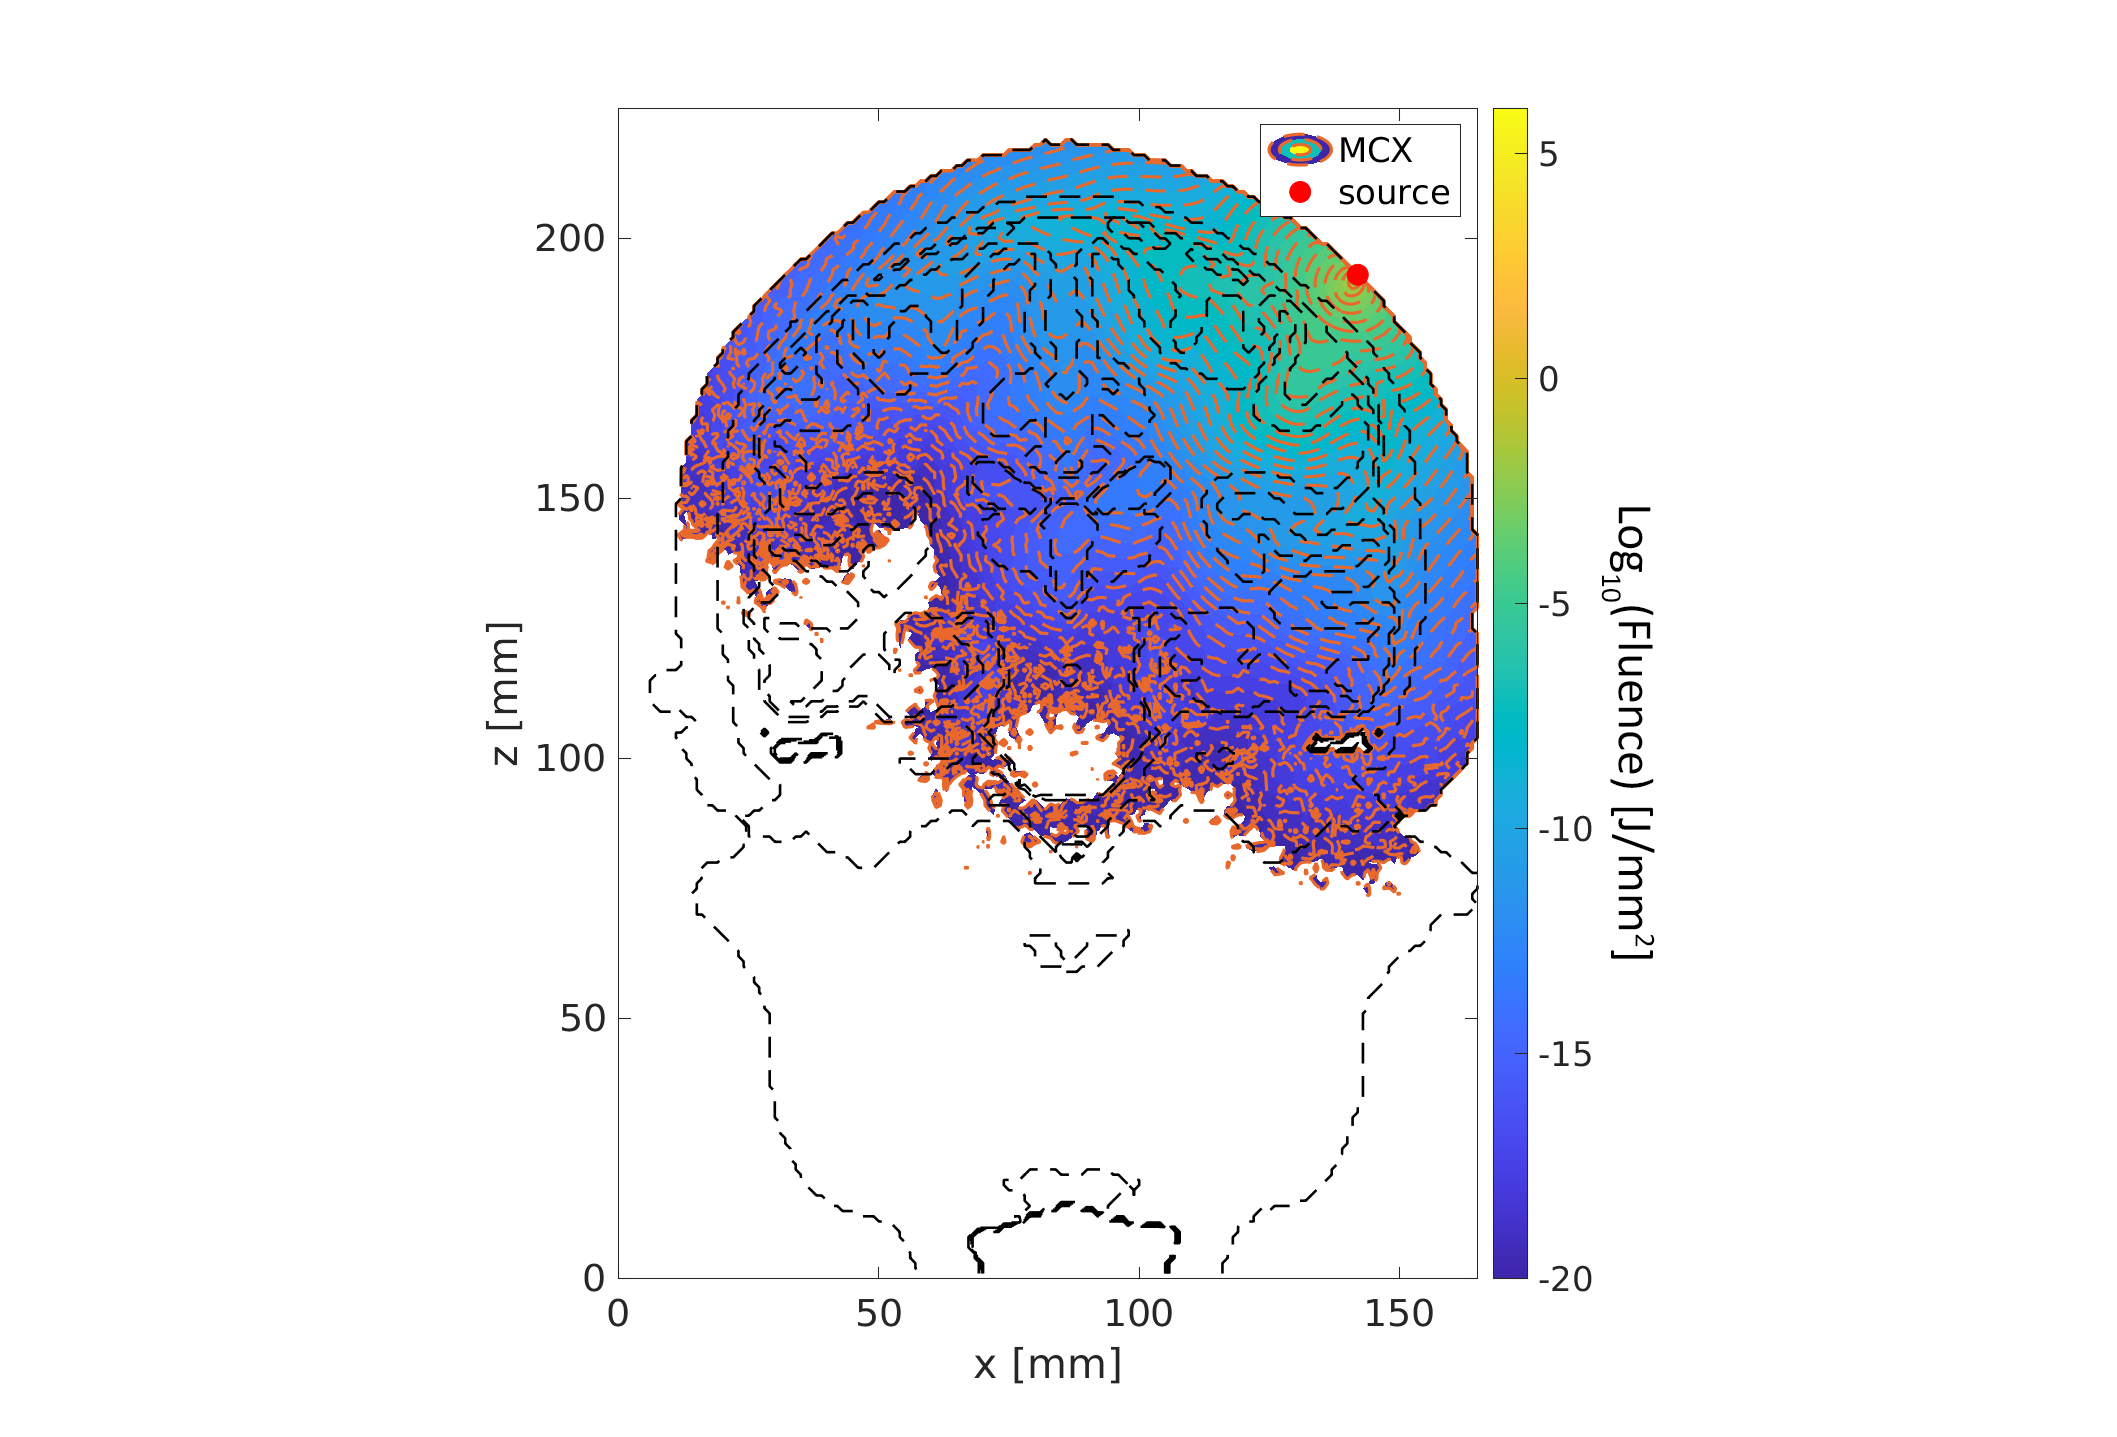
\includegraphics[width=\columnwidth]
    {Figures/Fluence_Distribution_1550nm_45deg.png}}
    \caption{\label{fig:1550-45} 1550 nm 45 Degree Position}
\end{figure}

\begin{figure}[htb!]
    \center{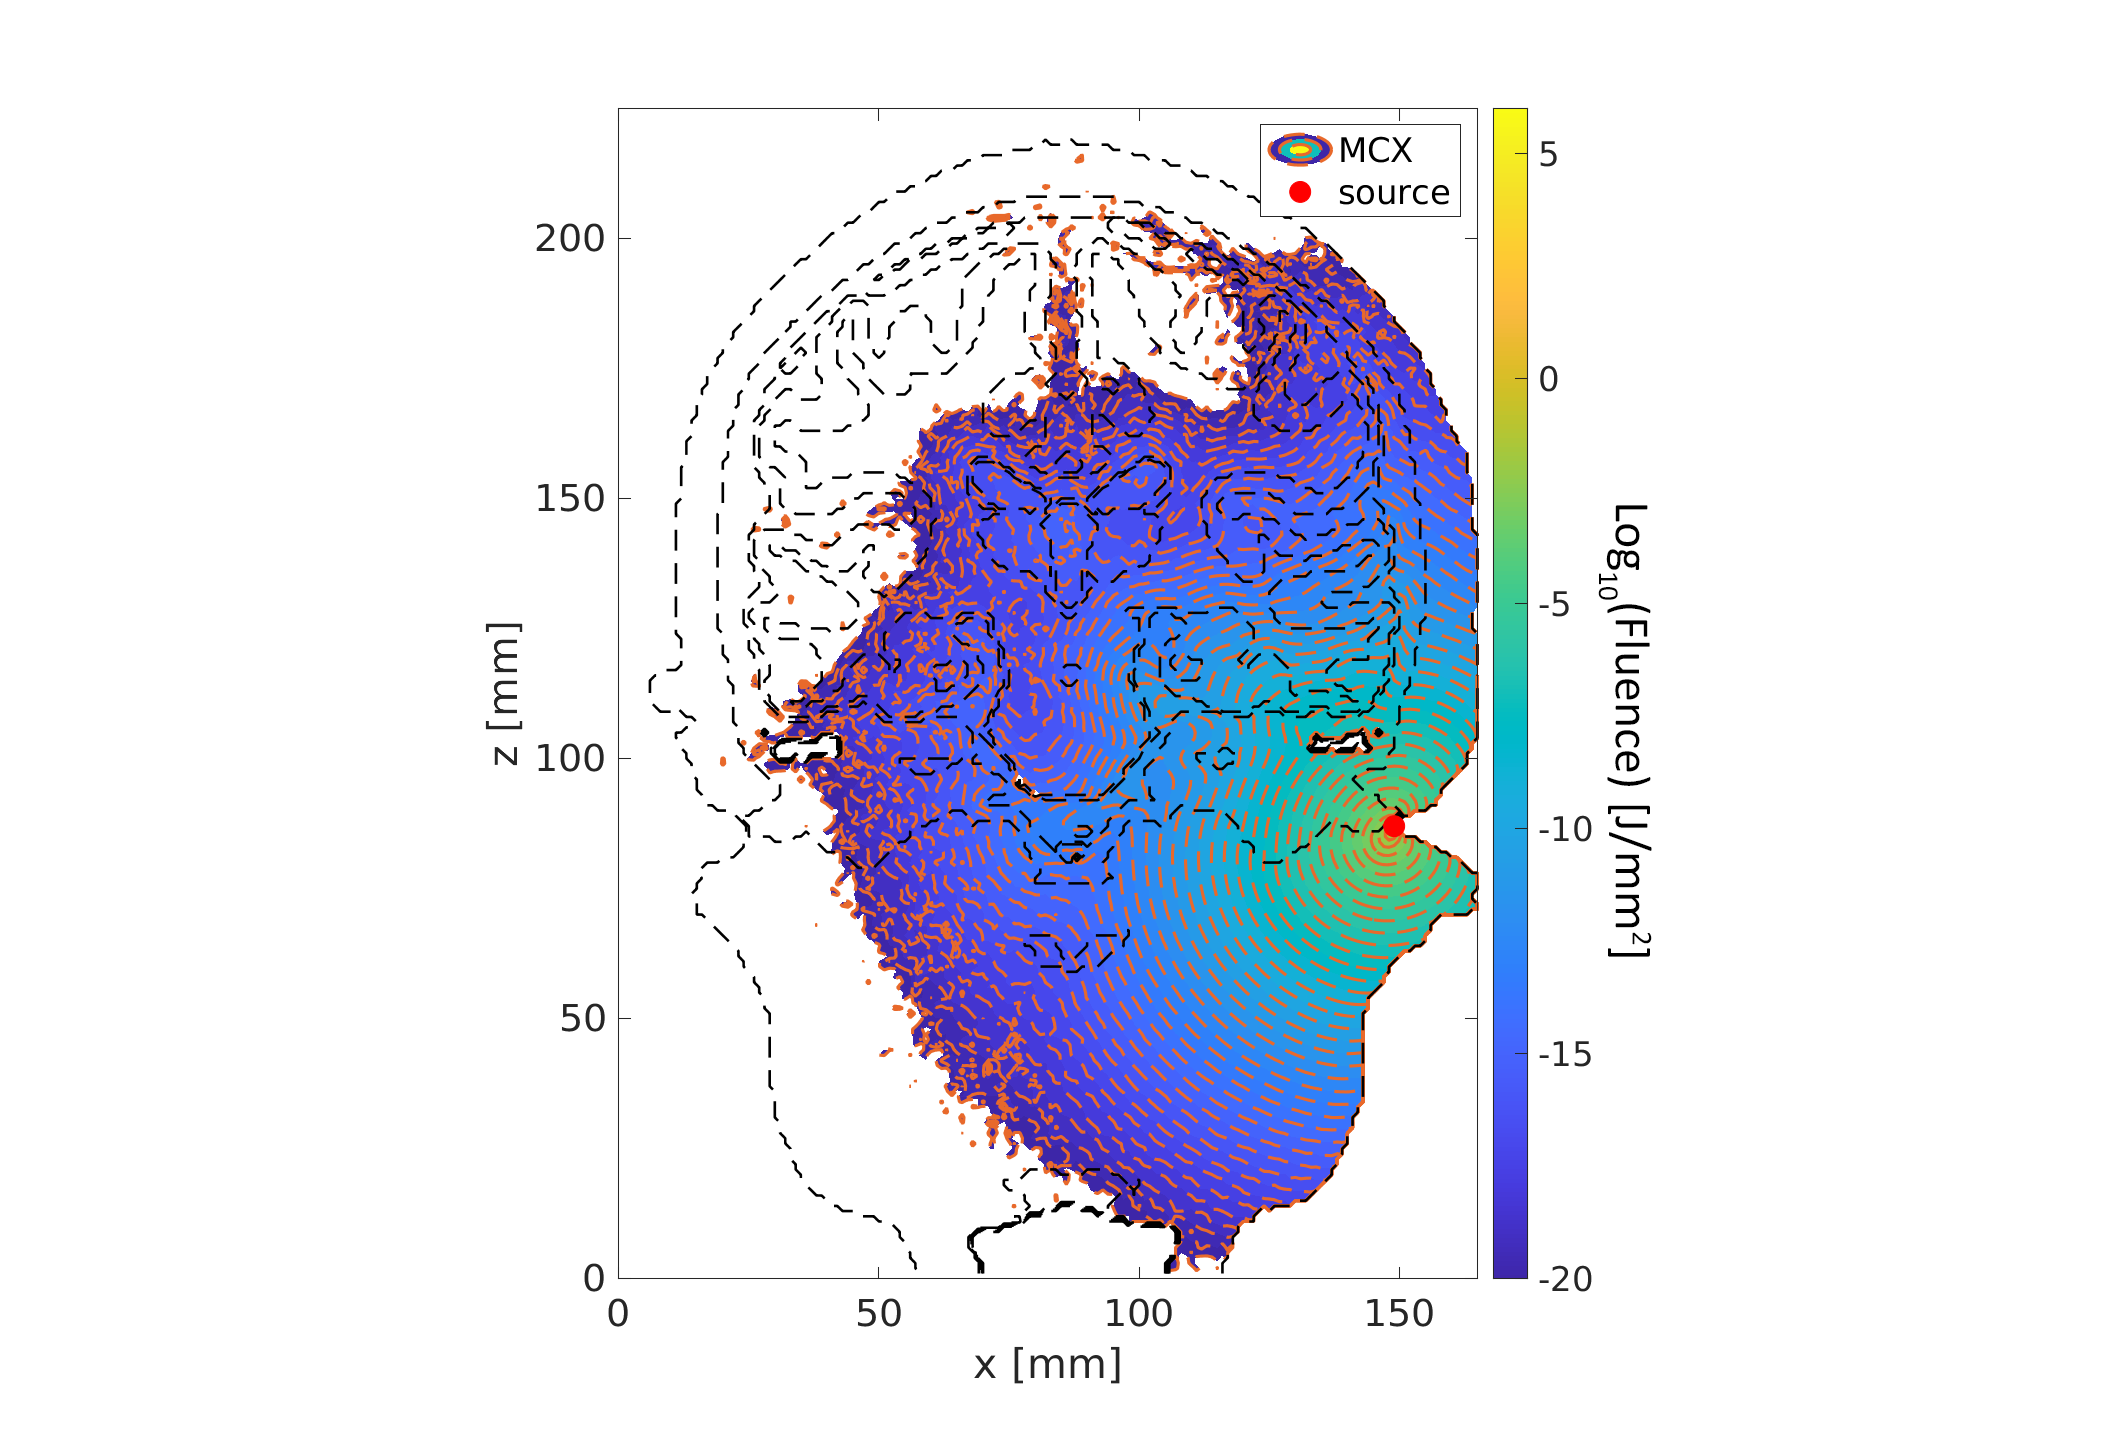
\includegraphics[width=\columnwidth]
    {Figures/Fluence_Distribution_1550nm_Cochlear.png}}
    \caption{\label{fig:1550-Cochlear} 1550 nm Cochlear Position}
\end{figure}

\begin{figure}[htb!]
    \center{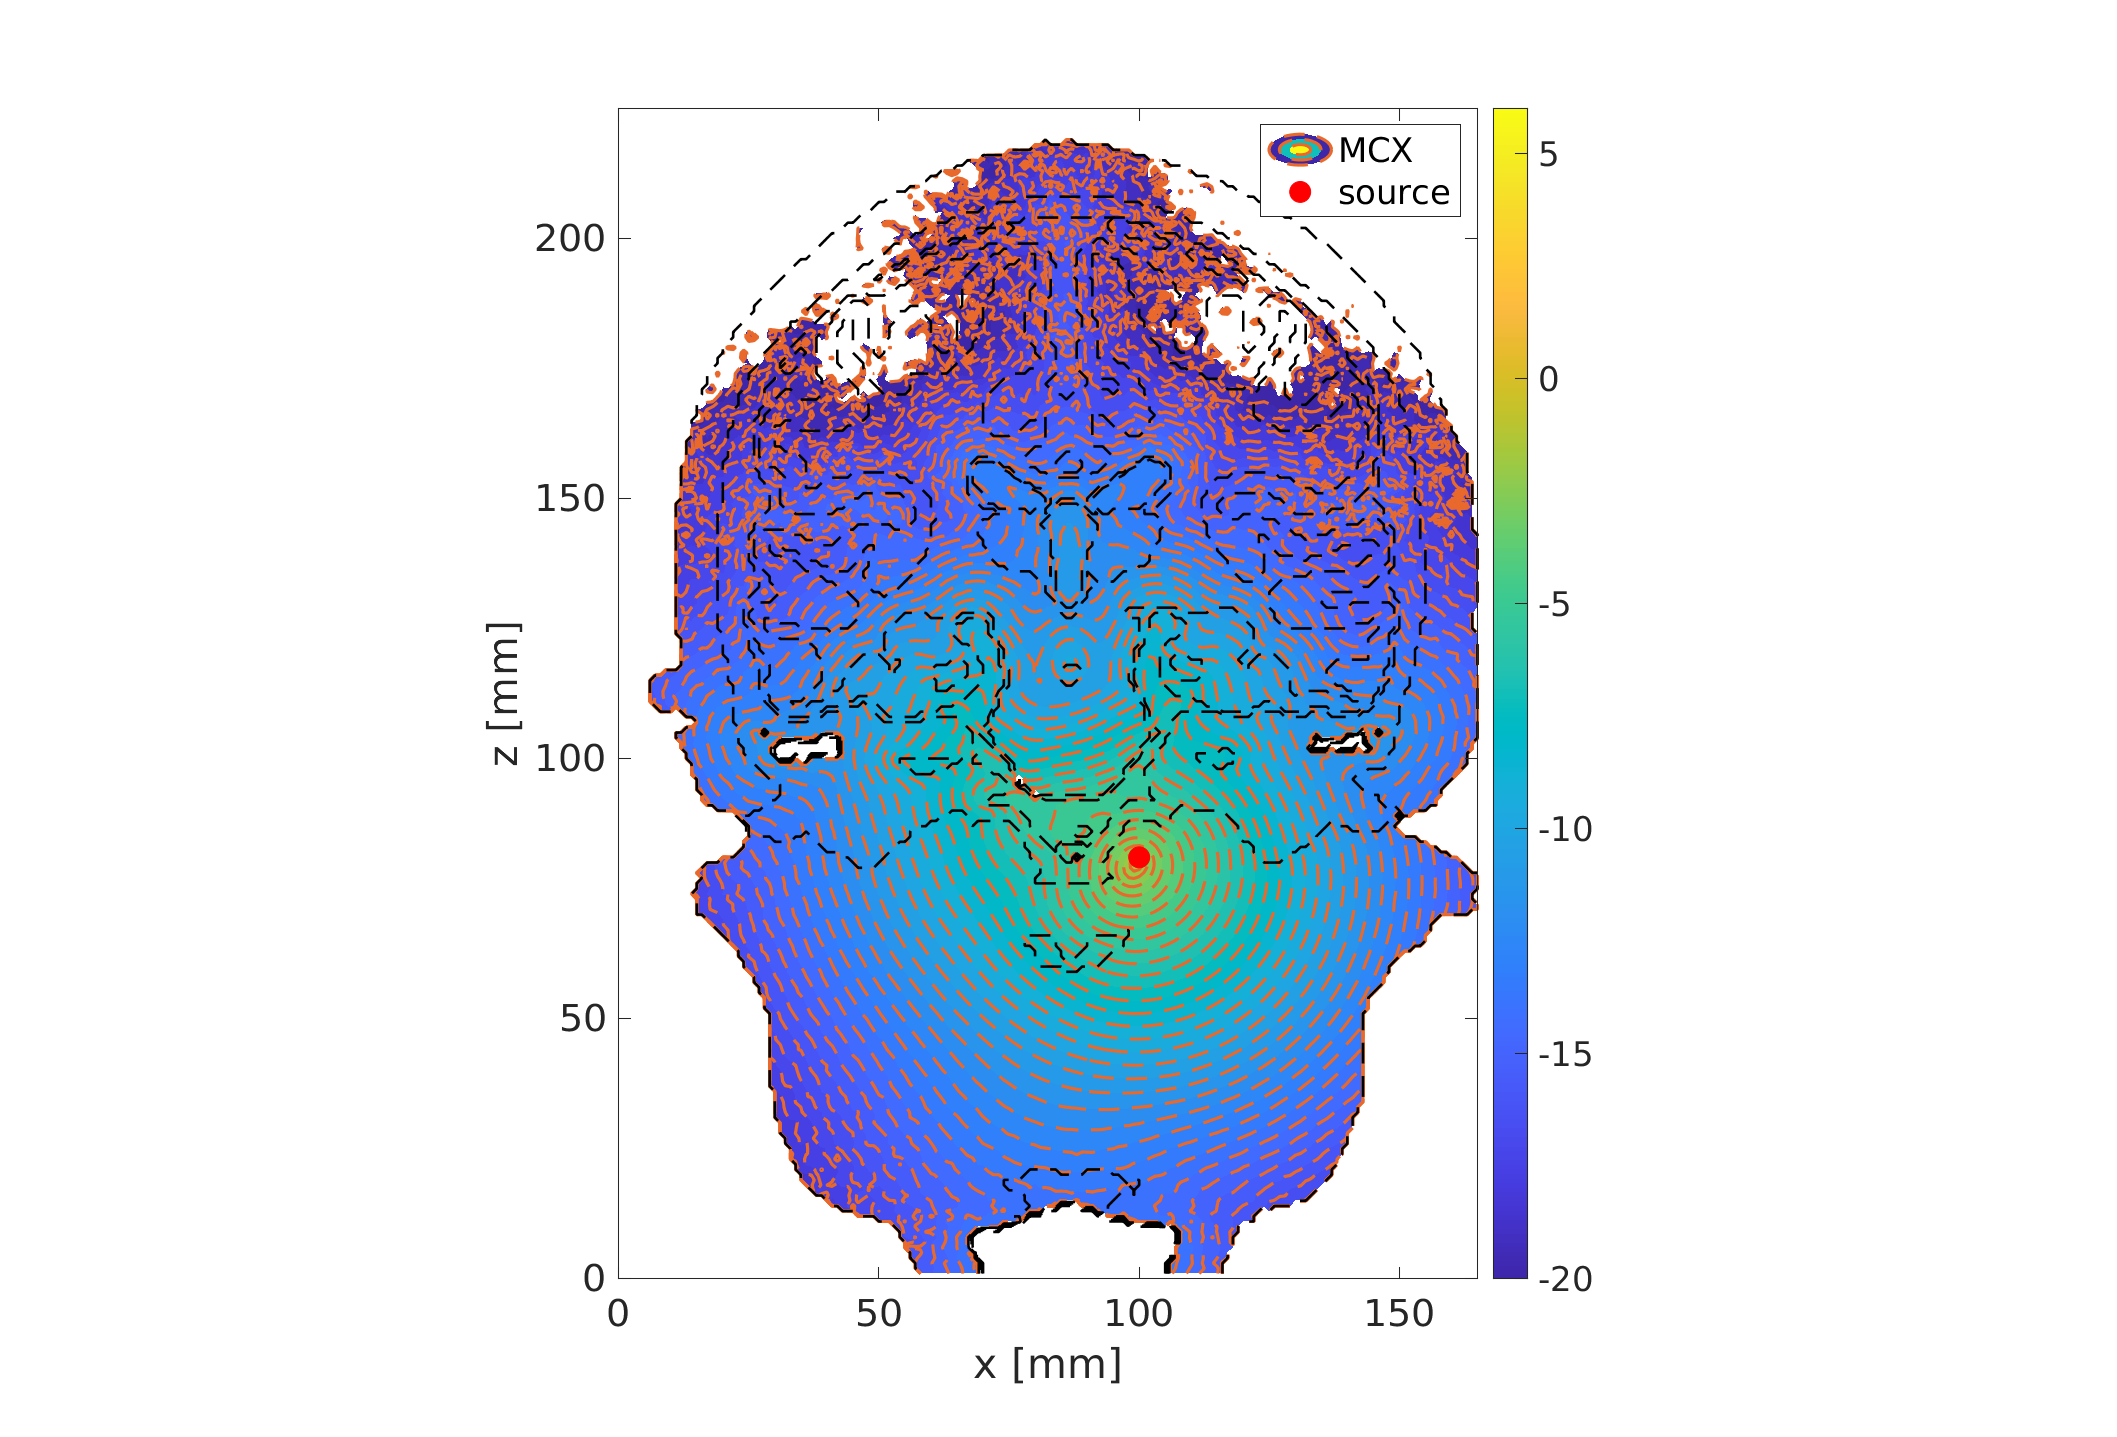
\includegraphics[width=\columnwidth]
    {Figures/Fluence_Distribution_1550nm_Intranasal.png}}
    \caption{\label{fig:1550-Intra} 1550 nm Intranasal Position}
\end{figure}


\end{document}
